\documentclass[12pt,a4paper]{report}

% =========================================================================
% GOI THU VIEN & CAU HINH CO BAN
% =========================================================================
% Tuong thich voi ca pdfLaTeX (Prism mac dinh) va XeLaTeX/LuaLaTeX.
\usepackage{iftex}
\ifPDFTeX
    \usepackage[utf8]{inputenc}
    \usepackage[T5]{fontenc}
    \usepackage{mathptmx}
\else
    \usepackage{fontspec}
    \IfFontExistsTF{Times New Roman}
        {\setmainfont{Times New Roman}}
        {\setmainfont{TeX Gyre Termes}}
\fi

\usepackage[top=2.5cm, bottom=2.5cm, left=3.0cm, right=2.0cm]{geometry}
\usepackage{amsmath, amsfonts, amssymb}
\usepackage{graphicx}
\usepackage{booktabs}
\usepackage{float}
\usepackage{xcolor}
\usepackage{hyperref}
\usepackage{fancyhdr}
\usepackage{titlesec}
\usepackage{caption}
\usepackage{listings}

% Ho tro ca khi Prism compile tu thu muc Report va tu thu muc goc project.
\graphicspath{{images/generated/}{images/}{Assignment3/Report/images/generated/}{Assignment3/Report/images/}}

% Cau hinh Hyperref
\hypersetup{
    colorlinks=true,
    linkcolor=black,
    citecolor=black,
    urlcolor=black,
    pdftitle={Bao Cao Ky Thuat Assignment 03 - Neural Networks and Representation Learning},
    pdfauthor={khoipv.447}
}

% Cau hinh Code Listing cho Python / NumPy
\definecolor{backcolour}{rgb}{0.96,0.97,0.98}

\lstdefinestyle{mystyle}{
    backgroundcolor=\color{backcolour},
    commentstyle=\color{black},
    keywordstyle=\color{black}\bfseries,
    numberstyle=\tiny\color{black},
    stringstyle=\color{black},
    basicstyle=\ttfamily\footnotesize\color{black},
    breakatwhitespace=false,
    breaklines=true,
    captionpos=b,
    keepspaces=true,
    numbers=left,
    numbersep=5pt,
    showspaces=false,
    showstringspaces=false,
    showtabs=false,
    tabsize=2,
    frame=single,
    rulecolor=\color{black}
}
\lstset{style=mystyle}

% Dinh dang tieu de chuong, muc
\titleformat{\chapter}[display]
  {\normalfont\bfseries\color{black}}
  {\filleft\Large\bfseries\chaptertitlename\ \thechapter}
  {1ex}
  {\titlerule\vspace{1ex}\filright\LARGE}
  [\vspace{1ex}\titlerule]

\titleformat{\section}
  {\normalfont\Large\bfseries\color{black}}
  {\thesection}{1em}{}

\titleformat{\subsection}
  {\normalfont\large\bfseries\color{black}}
  {\thesubsection}{1em}{}

% Header & Footer
\pagestyle{fancy}
\fancyhf{}
\fancyhead[R]{\small\itshape Assignment 03: Neural Networks and Representation Learning}
\fancyfoot[C]{\thepage}
\renewcommand{\headrulewidth}{0.4pt}
\renewcommand{\footrulewidth}{0.4pt}
\setlength{\headheight}{14pt}

\newcommand{\placeholder}[1]{\textcolor{black}{\textbf{[#1]}}}
\newcommand{\modelpath}[1]{\texttt{#1}}

% =========================================================================
% BAT DAU TAI LIEU
% =========================================================================
\begin{document}
\color{black}

% -------------------------------------------------------------------------
% MUC LUC & DANH MUC HINH ANH / BANG BIEU
% -------------------------------------------------------------------------
\pagenumbering{roman}
\tableofcontents
\newpage
\listoffigures
\newpage
\listoftables
\newpage
\pagenumbering{arabic}

% =========================================================================
% CHUONG 1
% =========================================================================
\chapter{Thiết Kế Thực Nghiệm Và Mạng Nơ-ron NumPy}

\section{Biểu diễn đầu vào và mô hình dự báo}
Trong các mô hình học máy truyền thống, chất lượng dự báo phụ thuộc mạnh vào tập đặc trưng đầu vào:
\begin{equation}
    \mathbf{X} \xrightarrow{\text{Feature Engineering}} \mathbf{X}_{engineered}
    \xrightarrow{\text{ML model}} \hat{y}.
\end{equation}
Với dữ liệu bảng, các đặc trưng như tuổi, chỉ số đường huyết, diện tích nhà hoặc vị trí địa lý có ý nghĩa trực tiếp. Với dữ liệu văn bản, mô hình cần một biểu diễn số hóa như TF-IDF để chuyển review thành vector đặc trưng.

Mạng nơ-ron đa tầng (Multi-Layer Perceptron -- MLP) mở rộng cách tiếp cận này bằng cách tự học các biểu diễn ẩn:
\begin{equation}
    \mathbf{X} \xrightarrow{h_{\theta}(\mathbf{X})} \mathbf{H}
    \xrightarrow{g_{\theta}(\mathbf{H})} \hat{y}.
\end{equation}
Các tham số $\theta = \{\mathbf{W}, \mathbf{b}\}$ được tối ưu đồng thời thông qua lan truyền tiến, hàm mất mát và lan truyền ngược.

\subsection{Biểu diễn được dùng cho từng bộ dữ liệu}
Assignment 03 gồm bốn thực nghiệm với các kiểu dữ liệu khác nhau, vì vậy biểu diễn đầu vào cũng được xử lý theo từng notebook.
Với \textit{diabetes} và \textit{diabetes large}, dữ liệu đã là bảng số hoặc bảng hỗn hợp số--phân loại.
Mô hình không cần chuyển đổi từ dạng tự nhiên như ảnh hoặc văn bản sang tensor phức tạp, nhưng vẫn phải học được tương tác giữa các đặc trưng y sinh.
Ví dụ, một giá trị \texttt{HbA1c\_level} cao có thể có ý nghĩa khác nhau tùy theo \texttt{age}, \texttt{bmi} và \texttt{blood\_glucose\_level}.

Với \textit{house price}, biểu diễn tốt không chỉ là chuẩn hóa số phòng ngủ hoặc diện tích.
Bài toán còn đòi hỏi xử lý biến phân loại nhiều giá trị như thành phố, zip code, broker, trạng thái giao dịch và thời gian bán trước.
Nếu chỉ one-hot toàn bộ biến high-cardinality, số chiều có thể tăng rất mạnh.
Notebook vì vậy dùng frequency encoding và trích xuất thời gian để tạo biểu diễn vừa đủ gọn, vừa giữ được tín hiệu vị trí và thị trường.

Với \textit{customer comments}, dữ liệu ban đầu là văn bản tự do.
Mỗi nhận xét cần được làm sạch, chuẩn hóa và ánh xạ sang vector TF-IDF 1,000 chiều.
Ở đây biểu diễn đóng vai trò trung tâm: cùng một câu văn, nếu giữ nguyên dạng chuỗi, các mô hình tuyến tính hoặc MLP NumPy không thể xử lý trực tiếp.
TF-IDF biến văn bản thành không gian thưa, trong đó mỗi chiều phản ánh mức độ quan trọng tương đối của một từ hoặc cụm từ trong tập train.

\subsection{Phạm vi dữ liệu}
Bảng \ref{tab:dataset_overview} gom các thông tin đầu vào được ghi nhận trong bốn notebook thuộc \modelpath{Assignment3}.
Bảng này nêu phạm vi chung; các bước EDA và tiền xử lý cụ thể được trình bày tại từng thực nghiệm.

\begin{table}[H]
\centering
\caption{Tổng quan các bộ dữ liệu trong Assignment 03}
\label{tab:dataset_overview}
\resizebox{\textwidth}{!}{%
\begin{tabular}{lllll}
\toprule
\textbf{Bộ dữ liệu} & \textbf{Dạng bài toán} & \textbf{Kích thước dùng trong notebook} & \textbf{Target} & \textbf{Đặc điểm chính} \\
\midrule
Customer comments & Phân loại nhị phân & 22,642 review hợp lệ & \texttt{Recommended IND} & Văn bản thưa TF-IDF, nhãn mất cân bằng \\
House price & Hồi quy & Sample 200,000 từ 2,226,382 dòng & \texttt{price} & Giá lệch phải, nhiều missing và outlier \\
Diabetes & Phân loại nhị phân & 768 mẫu, 8 feature & \texttt{Outcome} & Dữ liệu y sinh nhỏ, có giá trị 0 bất thường \\
Diabetes large & Phân loại nhị phân & 100,000 mẫu & \texttt{diabetes} & Mất cân bằng mạnh, feature số và phân loại \\
\bottomrule
\end{tabular}%
}
\end{table}

\subsection{Quy trình đối chuẩn}
Các notebook triển khai đối chuẩn theo cùng một quy trình:
\begin{enumerate}
    \item Dữ liệu được chia train, validation và test hoặc train/test trước khi fit các bước tiền xử lý có trạng thái.
    \item Các mô hình truyền thống và MLP NumPy dùng cùng tập đặc trưng sau tiền xử lý.
    \item Metric được chọn theo bản chất bài toán, ví dụ F1/PR-AUC cho phân loại mất cân bằng và RMSLE/MAE cho hồi quy giá nhà.
    \item Thời gian huấn luyện và dự đoán được ghi nhận để so sánh cả chất lượng mô hình lẫn chi phí tính toán.
    \item Các đồ thị sinh ra trong notebook được lưu vào \modelpath{report/figures}; các ảnh dùng trong báo cáo nằm tại \modelpath{Assignment3/Report/images/generated}.
\end{enumerate}

Những nguyên tắc này giúp tránh tình huống chỉ báo cáo một con số accuracy đẹp nhưng không phản ánh đúng chất lượng mô hình.
Đặc biệt với dữ liệu mất cân bằng, mô hình có thể đạt accuracy cao bằng cách dự đoán hầu hết mẫu là lớp đa số.
Vì vậy, báo cáo luôn đọc kèm precision, recall, F1, ROC-AUC hoặc PR-AUC thay vì kết luận vội từ accuracy.

\section{Các phép tính trong MLP NumPy}
Với một tầng $l$, MLP thực hiện biến đổi affine và kích hoạt phi tuyến:
\begin{align}
    \mathbf{Z}^{[l]} &= \mathbf{A}^{[l-1]}\mathbf{W}^{[l]} + \mathbf{b}^{[l]}, \\
    \mathbf{A}^{[l]} &= \phi(\mathbf{Z}^{[l]}).
\end{align}
Nếu bỏ hàm kích hoạt phi tuyến, nhiều tầng tuyến tính chỉ tương đương một phép biến đổi tuyến tính duy nhất. Vì vậy ReLU được dùng ở các tầng ẩn:
\begin{equation}
    ReLU(z) = \max(0, z), \quad
    ReLU'(z) =
    \begin{cases}
        1 & z > 0,\\
        0 & z \le 0.
    \end{cases}
\end{equation}

\subsection{Biến đổi affine và kích hoạt ẩn}
Mỗi tầng trong MLP có thể được nhìn như một phép chiếu dữ liệu sang không gian mới.
Ma trận trọng số $\mathbf{W}^{[l]}$ quyết định cách kết hợp các đặc trưng đầu vào, còn vector bias $\mathbf{b}^{[l]}$ dịch chuyển siêu phẳng quyết định.
Trong một bài toán bảng, một neuron ẩn có thể học tổ hợp giữa \texttt{age}, \texttt{bmi}, \texttt{glucose} hoặc các cột one-hot.
Trong bài toán văn bản, một neuron có thể học tổ hợp giữa các từ biểu thị cảm xúc tích cực và tiêu cực.

Nếu số neuron ở tầng ẩn quá ít, mô hình thiếu khả năng biểu diễn quan hệ phi tuyến.
Nếu số neuron quá nhiều so với kích thước dữ liệu, mô hình dễ ghi nhớ train set và suy giảm trên test set.
Do đó các kiến trúc trong notebook được chọn ở mức vừa phải: diabetes large dùng $64 \to 32 \to 16$, house price dùng $128 \to 64 \to 32$, còn customer comments dùng $64 \to 16$ vì vector TF-IDF 1,000 chiều đã rất giàu thông tin.

\subsection{ReLU, sigmoid và tầng đầu ra tuyến tính}
ReLU được dùng ở tầng ẩn vì đạo hàm đơn giản và giảm hiện tượng gradient nhỏ dần so với sigmoid ở mọi tầng.
Trong forward pass, ReLU giữ lại giá trị dương và chặn các giá trị âm về 0.
Điều này tạo ra tính thưa trong kích hoạt ẩn, giúp một số neuron chỉ phản ứng với một vùng dữ liệu nhất định.

Sigmoid phù hợp với phân loại nhị phân vì đầu ra nằm trong khoảng $[0,1]$ và có thể diễn giải như xác suất thuộc lớp dương.
Tuy nhiên xác suất này không tự động quyết định ngưỡng phân loại.
Ngưỡng mặc định 0.5 chỉ là một lựa chọn tiện lợi; với dữ liệu mất cân bằng, notebook chọn ngưỡng dựa trên validation set để tối ưu F1 hoặc cân bằng precision--recall.

Trong hồi quy giá nhà, tầng đầu ra không dùng sigmoid vì giá trị cần dự đoán là liên tục.
Notebook huấn luyện trên $log1p(price)$ với output tuyến tính, sau đó dùng hàm nghịch đảo $expm1$ để đưa dự đoán về đơn vị USD.
Thiết kế này giúp mô hình tập trung vào sai số tương đối của giá thay vì bị các căn nhà cực đắt chi phối hoàn toàn.

\section{Lan truyền tiến, lan truyền ngược và cập nhật tham số}
Với bài toán phân loại nhị phân, tầng đầu ra dùng sigmoid:
\begin{equation}
    \hat{y} = \sigma(z) = \frac{1}{1 + e^{-z}},
\end{equation}
và tối ưu Binary Cross-Entropy:
\begin{equation}
    \mathcal{L}_{BCE} =
    -\frac{1}{m}\sum_{i=1}^{m}
    \left[y^{(i)}\log(\hat{y}^{(i)}+\epsilon)
    +(1-y^{(i)})\log(1-\hat{y}^{(i)}+\epsilon)\right].
\end{equation}
Với bài toán hồi quy giá nhà, đầu ra tuyến tính và hàm mất mát MSE được áp dụng trên biến đổi $log1p(price)$ để giảm ảnh hưởng của outlier.

Mini-batch Gradient Descent chia dữ liệu thành các batch nhỏ để cập nhật tham số:
\begin{equation}
    \theta \leftarrow \theta - \eta \nabla_{\theta}\mathcal{L}.
\end{equation}
Việc hiện thực bằng NumPy giúp kiểm soát rõ dòng chảy ma trận, gradient, regularization và ảnh hưởng của từng quyết định tiền xử lý.

\subsection{Forward pass dạng mã giả NumPy}
Đoạn mã \ref{lst:forward} minh họa forward pass tổng quát cho một MLP phân loại nhị phân.
Trong notebook thực tế, cấu trúc được đóng gói bằng class để tái sử dụng cho nhiều batch và theo dõi lịch sử train/validation.

\begin{lstlisting}[language=Python, caption={Forward pass MLP phân loại nhị phân bằng NumPy}, label={lst:forward}]
def relu(z):
    return np.maximum(0.0, z)

def sigmoid(z):
    z = np.clip(z, -500, 500)
    return 1.0 / (1.0 + np.exp(-z))

def forward(X, params):
    Z1 = X @ params["W1"] + params["b1"]
    A1 = relu(Z1)
    Z2 = A1 @ params["W2"] + params["b2"]
    A2 = relu(Z2)
    logits = A2 @ params["W3"] + params["b3"]
    y_proba = sigmoid(logits)
    cache = (X, Z1, A1, Z2, A2, logits, y_proba)
    return y_proba, cache
\end{lstlisting}

\subsection{Backpropagation và kiểm soát gradient}
Backpropagation áp dụng quy tắc dây chuyền để tính gradient từ output ngược về từng tầng.
Với sigmoid kết hợp Binary Cross-Entropy, đạo hàm theo logits có dạng gọn:
\begin{equation}
    \frac{\partial \mathcal{L}}{\partial z} = \hat{y} - y.
\end{equation}
Khi thêm class weighting, sai số của từng mẫu được nhân với trọng số lớp tương ứng.
Điều này làm cho mẫu lớp thiểu số có đóng góp lớn hơn vào gradient, giúp mô hình không bỏ qua lớp dương trong các bài toán như diabetes large.

L2 regularization được thêm trực tiếp vào gradient trọng số:
\begin{equation}
    \nabla_{\mathbf{W}}\mathcal{L}_{total}
    =
    \nabla_{\mathbf{W}}\mathcal{L}_{data}
    +
    \lambda \mathbf{W}.
\end{equation}
Thành phần này kéo trọng số về gần 0, giảm nguy cơ mô hình tạo ra biên quyết định quá phức tạp so với dữ liệu train.
Trong các notebook, regularization được dùng như một ràng buộc nhẹ thay vì ép mô hình quá đơn giản.

\subsection{Cập nhật theo mini-batch}
Mini-batch Gradient Descent là điểm cân bằng giữa Batch Gradient Descent và Stochastic Gradient Descent.
Batch toàn bộ ổn định nhưng tốn bộ nhớ và cập nhật chậm trên dữ liệu lớn.
Stochastic từng mẫu cập nhật nhanh nhưng nhiễu lớn.
Trong code, kích thước batch lần lượt là 64 cho diabetes nhỏ, 1,024 cho diabetes large, 2,048 cho house price và 256 cho customer comments.

\begin{lstlisting}[language=Python, caption={Vòng lặp mini-batch gradient descent}, label={lst:minibatch}]
for epoch in range(max_epochs):
    indices = rng.permutation(n_train)
    X_train = X_train[indices]
    y_train = y_train[indices]

    for start in range(0, n_train, batch_size):
        end = start + batch_size
        X_batch = X_train[start:end]
        y_batch = y_train[start:end]

        y_proba, cache = forward(X_batch, params)
        grads = backward(y_batch, y_proba, cache, params)

        for name in params:
            params[name] -= learning_rate * grads[name]
\end{lstlisting}

\subsection{Đánh giá metric theo bản chất bài toán}
Bảng \ref{tab:metric_meaning} trình bày ý nghĩa các metric chính trong báo cáo.
Việc dùng nhiều metric giúp nhìn được các góc khác nhau: khả năng phát hiện lớp dương, mức độ báo động sai, độ ổn định theo ngưỡng và mức sai số tiền tệ.

\begin{table}[H]
\centering
\caption{Ý nghĩa các metric dùng trong báo cáo}
\label{tab:metric_meaning}
\resizebox{\textwidth}{!}{%
\begin{tabular}{lll}
\toprule
\textbf{Metric} & \textbf{Dùng cho} & \textbf{Ý nghĩa diễn giải} \\
\midrule
Accuracy & Phân loại & Tỷ lệ dự đoán đúng tổng thể, dễ bị đánh lừa khi dữ liệu mất cân bằng \\
Precision & Phân loại & Trong các mẫu dự đoán dương, bao nhiêu mẫu thật sự dương \\
Recall & Phân loại & Trong các mẫu dương thật, mô hình phát hiện được bao nhiêu mẫu \\
F1-Score & Phân loại & Trung bình điều hòa giữa precision và recall, hữu ích khi cần cân bằng hai loại sai lỗi \\
ROC-AUC & Phân loại & Khả năng xếp hạng mẫu dương cao hơn mẫu âm trên nhiều ngưỡng \\
PR-AUC & Phân loại mất cân bằng & Diện tích dưới đường precision--recall, nhạy hơn ROC-AUC khi lớp dương hiếm \\
MAE & Hồi quy & Sai số tuyệt đối trung bình theo đơn vị gốc, dễ diễn giải bằng USD với house price \\
RMSE & Hồi quy & Phạt mạnh sai số lớn, nhạy với outlier \\
MedianAE & Hồi quy & Sai số tuyệt đối trung vị, ít bị outlier kéo lệch \\
MAPE & Hồi quy & Sai số phần trăm trung bình, cần cẩn trọng khi giá trị thật rất nhỏ \\
RMSLE & Hồi quy giá lệch phải & Sai số trên log scale, nhấn mạnh tỷ lệ sai hơn sai số tuyệt đối \\
$R^2$ & Hồi quy & Tỷ lệ phương sai target được mô hình giải thích so với baseline trung bình \\
\bottomrule
\end{tabular}%
}
\end{table}

\subsection{Chống rò rỉ dữ liệu}
Data leakage xảy ra khi thông tin từ validation hoặc test lọt vào quá trình huấn luyện.
Ví dụ, nếu scaler được fit trên toàn bộ dữ liệu trước khi split, trung bình và độ lệch chuẩn của test set đã gián tiếp tham gia vào train.
Điều này làm kết quả đánh giá lạc quan hơn thực tế.
Các notebook vì vậy luôn tách dữ liệu trước rồi mới fit scaler, encoder hoặc TF-IDF trên train.

\begin{lstlisting}[language=Python, caption={Nguyên tắc fit trên train, transform trên validation/test}, label={lst:leakage}]
X_train_raw, X_test_raw, y_train, y_test = train_test_split(
    X_raw, y, test_size=0.2, stratify=y, random_state=42
)

scaler.fit(X_train_raw[numeric_columns])
X_train_num = scaler.transform(X_train_raw[numeric_columns])
X_test_num = scaler.transform(X_test_raw[numeric_columns])

tfidf.fit(train_text)
X_train_text = tfidf.transform(train_text)
X_test_text = tfidf.transform(test_text)
\end{lstlisting}

% =========================================================================
% CHUONG 2
% =========================================================================
\chapter{Diabetes Nhỏ: Từ Baseline Đến MLP Cải Tiến}

\section{Dữ liệu và hai cấu hình thực nghiệm}
Thư mục \modelpath{Assignment3/diabetes/notebook} chứa hai notebook:
\begin{itemize}
    \item \modelpath{diabetes\_numpy\_deep\_learning.ipynb}: baseline MLP thuần NumPy.
    \item \modelpath{diabetes\_improved.ipynb}: phiên bản cải tiến có validation split, tiền xử lý tốt hơn, threshold tuning và trực quan hóa.
\end{itemize}
Bộ dữ liệu \modelpath{diabetes.csv} là dữ liệu Pima Diabetes gồm 768 mẫu, 8 đặc trưng đầu vào và nhãn nhị phân \texttt{Outcome}.

\subsection{Mục đích của thực nghiệm quy mô nhỏ}
Bộ diabetes nhỏ được dùng như bước khởi động để kiểm chứng toàn bộ pipeline MLP thuần NumPy.
Kích thước 768 mẫu đủ nhỏ để chạy nhanh, quan sát được từng thay đổi về loss, accuracy và confusion matrix.
Điều này rất phù hợp cho mục tiêu học thuật: trước khi áp dụng MLP lên dữ liệu lớn hơn, notebook cần chứng minh rằng forward pass, backpropagation, cập nhật trọng số và đánh giá test set hoạt động đúng.

Khác với các mô hình scikit-learn, MLP NumPy không có sẵn cơ chế tự kiểm soát dữ liệu đầu vào.
Nếu feature chưa được chuẩn hóa, gradient ở các chiều có thang đo lớn sẽ chi phối quá trình học.
Nếu thiếu validation set, việc chọn số epoch hoặc threshold có thể vô tình dựa trên test set.
Vì vậy phiên bản cải tiến của notebook bổ sung rõ ràng các bước tiền xử lý, validation tracking và threshold tuning.

\subsection{Pipeline tiền xử lý của bốn bài toán}
Bảng \ref{tab:preprocessing_pipeline} tổng hợp các bước tiền xử lý chính.
Điểm chung quan trọng nhất là mọi phép biến đổi có trạng thái đều chỉ được fit trên train set.
Điểm khác nhau nằm ở bản chất dữ liệu: dữ liệu y sinh cần xử lý giá trị 0 bất thường, dữ liệu giá nhà cần log-transform và encoding biến phân loại, còn dữ liệu review cần làm sạch văn bản và TF-IDF.

\begin{table}[H]
\centering
\caption{Pipeline tiền xử lý theo từng bài toán}
\label{tab:preprocessing_pipeline}
\resizebox{\textwidth}{!}{%
\begin{tabular}{llll}
\toprule
\textbf{Bài toán} & \textbf{Split} & \textbf{Feature processing} & \textbf{Chống leakage} \\
\midrule
Diabetes & Train/Validation/Test & Thay 0 bất thường bằng median, scale feature số & Median/scaler học từ train \\
Diabetes large & 70/15/15 stratified & One-hot categorical, scale numeric & Encoder/scaler fit trên train \\
House price & Train/Validation/Test & Impute, log feature lệch, one-hot, frequency encoding & Imputer/encoder/statistics fit trên train \\
Customer comments & 80/20 stratified & Clean text, TF-IDF đúng 1,000 vocabulary & TF-IDF fit trên train, test chỉ transform \\
\bottomrule
\end{tabular}%
}
\end{table}

\section{Kiểm tra dữ liệu trước huấn luyện}
Các biểu đồ EDA cho thấy tập dữ liệu có mất cân bằng nhãn và nhiều cột y sinh có giá trị 0 bất thường. Với các cột như glucose, blood pressure, skin thickness, insulin và BMI, giá trị 0 không mang ý nghĩa sinh học hợp lý nên được xử lý như missing value trước khi chuẩn hóa.

\subsection{Giá trị 0 bất thường trong dữ liệu y sinh}
Trong bộ Pima Diabetes, một số cột như \texttt{Glucose}, \texttt{BloodPressure}, \texttt{SkinThickness}, \texttt{Insulin} và \texttt{BMI} có giá trị bằng 0.
Về mặt dữ liệu, số 0 có thể xuất hiện do thiếu đo đạc hoặc lỗi nhập liệu.
Về mặt y sinh, các giá trị như glucose hoặc BMI bằng 0 không hợp lý cho một bệnh nhân sống.
Nếu giữ nguyên, mô hình có thể học nhầm rằng 0 là một trạng thái sinh học bình thường, làm méo phân phối feature.

Notebook cải tiến xử lý các giá trị này như missing value.
Sau đó, missing được thay bằng median tính trên train set.
Median được ưu tiên hơn mean vì ít bị ảnh hưởng bởi outlier, đặc biệt với \texttt{Insulin} có phân phối lệch.
Sau bước này, các feature được chuẩn hóa để quá trình tối ưu của MLP ổn định hơn.

\subsection{Tách validation set để ra quyết định}
Một điểm khác biệt quan trọng giữa baseline và improved notebook là validation set.
Test set chỉ nên dùng một lần ở cuối để báo cáo kết quả khách quan.
Các quyết định như chọn epoch dừng sớm, chọn threshold hoặc theo dõi overfitting cần dựa vào validation set.
Vì vậy notebook cải tiến tách dữ liệu thành train, validation và test, đồng thời giữ phân phối nhãn tương đối ổn định giữa các tập.

Với dữ liệu nhỏ, từng mẫu trong lớp dương đều quan trọng.
Stratified split giúp giảm rủi ro validation hoặc test set có quá ít mẫu bệnh.
Nếu split ngẫu nhiên không phân tầng, metric recall và F1 có thể dao động mạnh chỉ vì phân phối nhãn bị lệch trong một lần chia dữ liệu.

\begin{figure}[H]
    \centering
    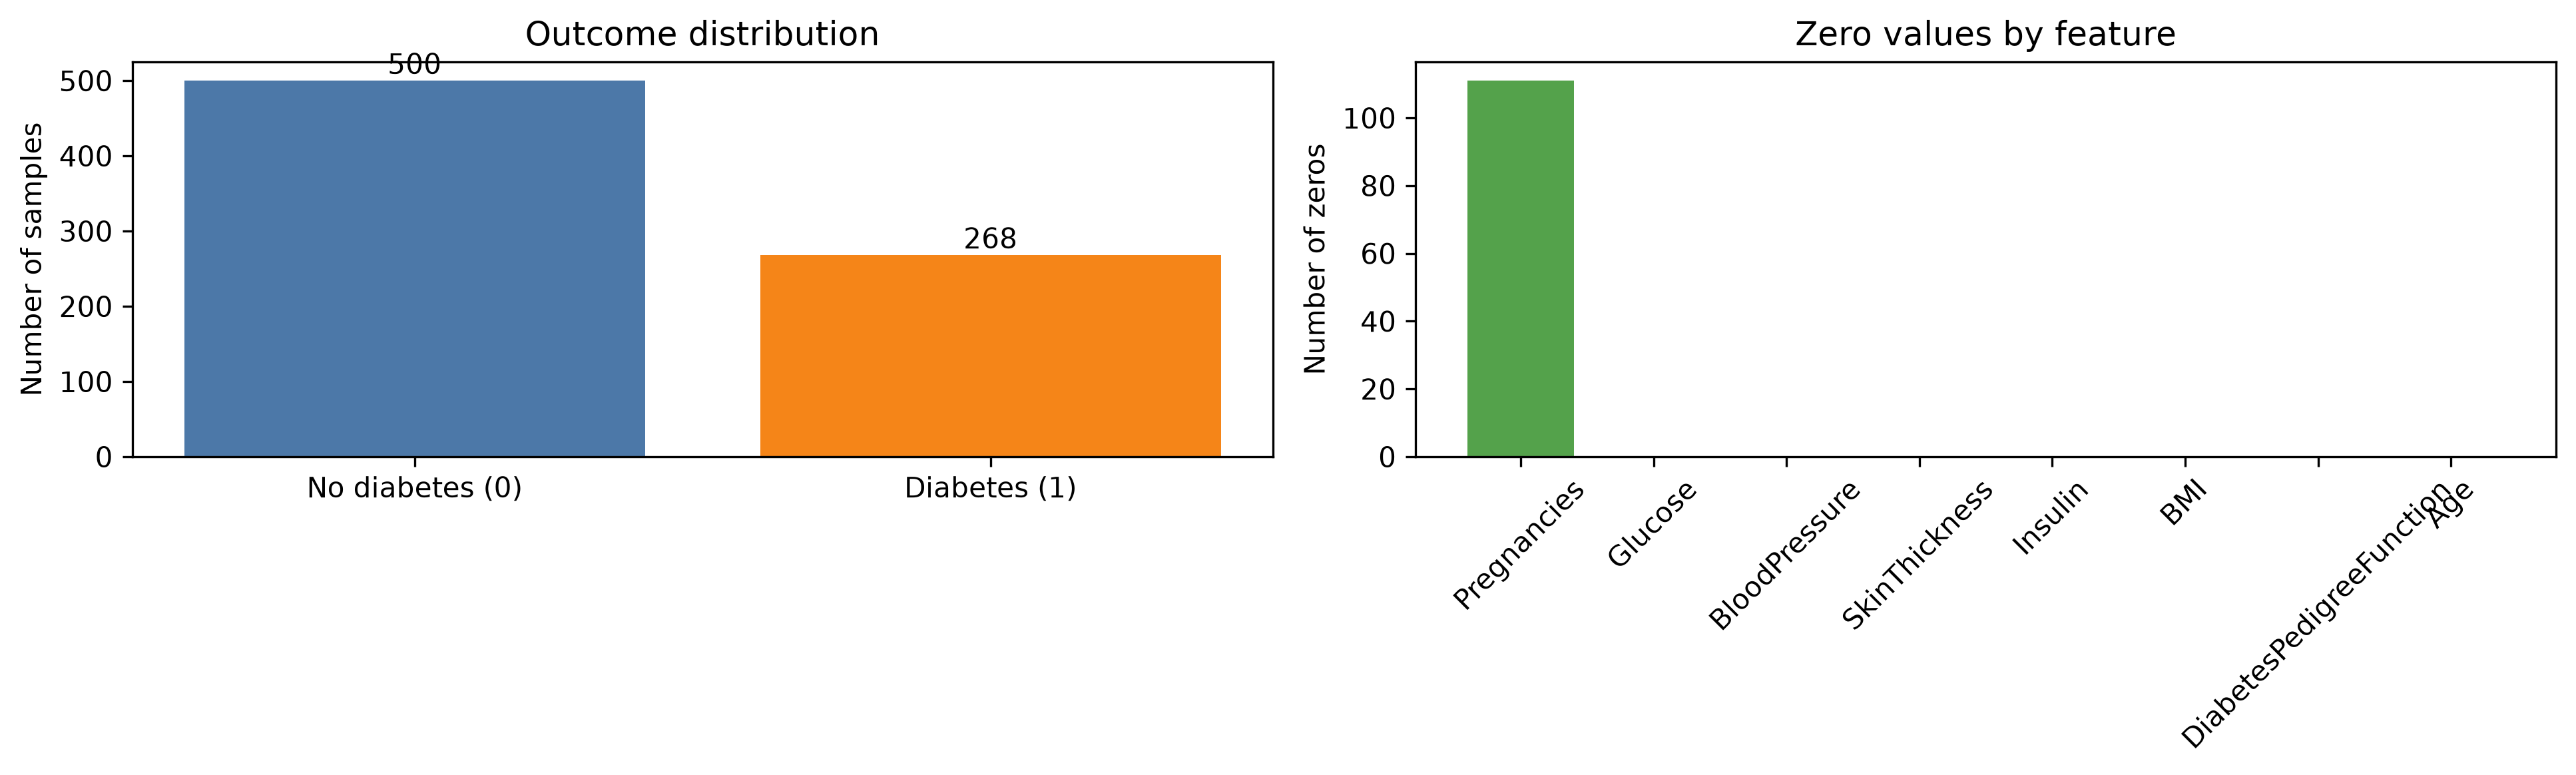
\includegraphics[width=0.92\textwidth]{diabetes_raw_outcome_zero_values.png}
    \caption{Phân phối nhãn Outcome và số lượng giá trị 0 theo đặc trưng}
    \label{fig:diabetes_raw_outcome_zero}
\end{figure}

\begin{figure}[H]
    \centering
    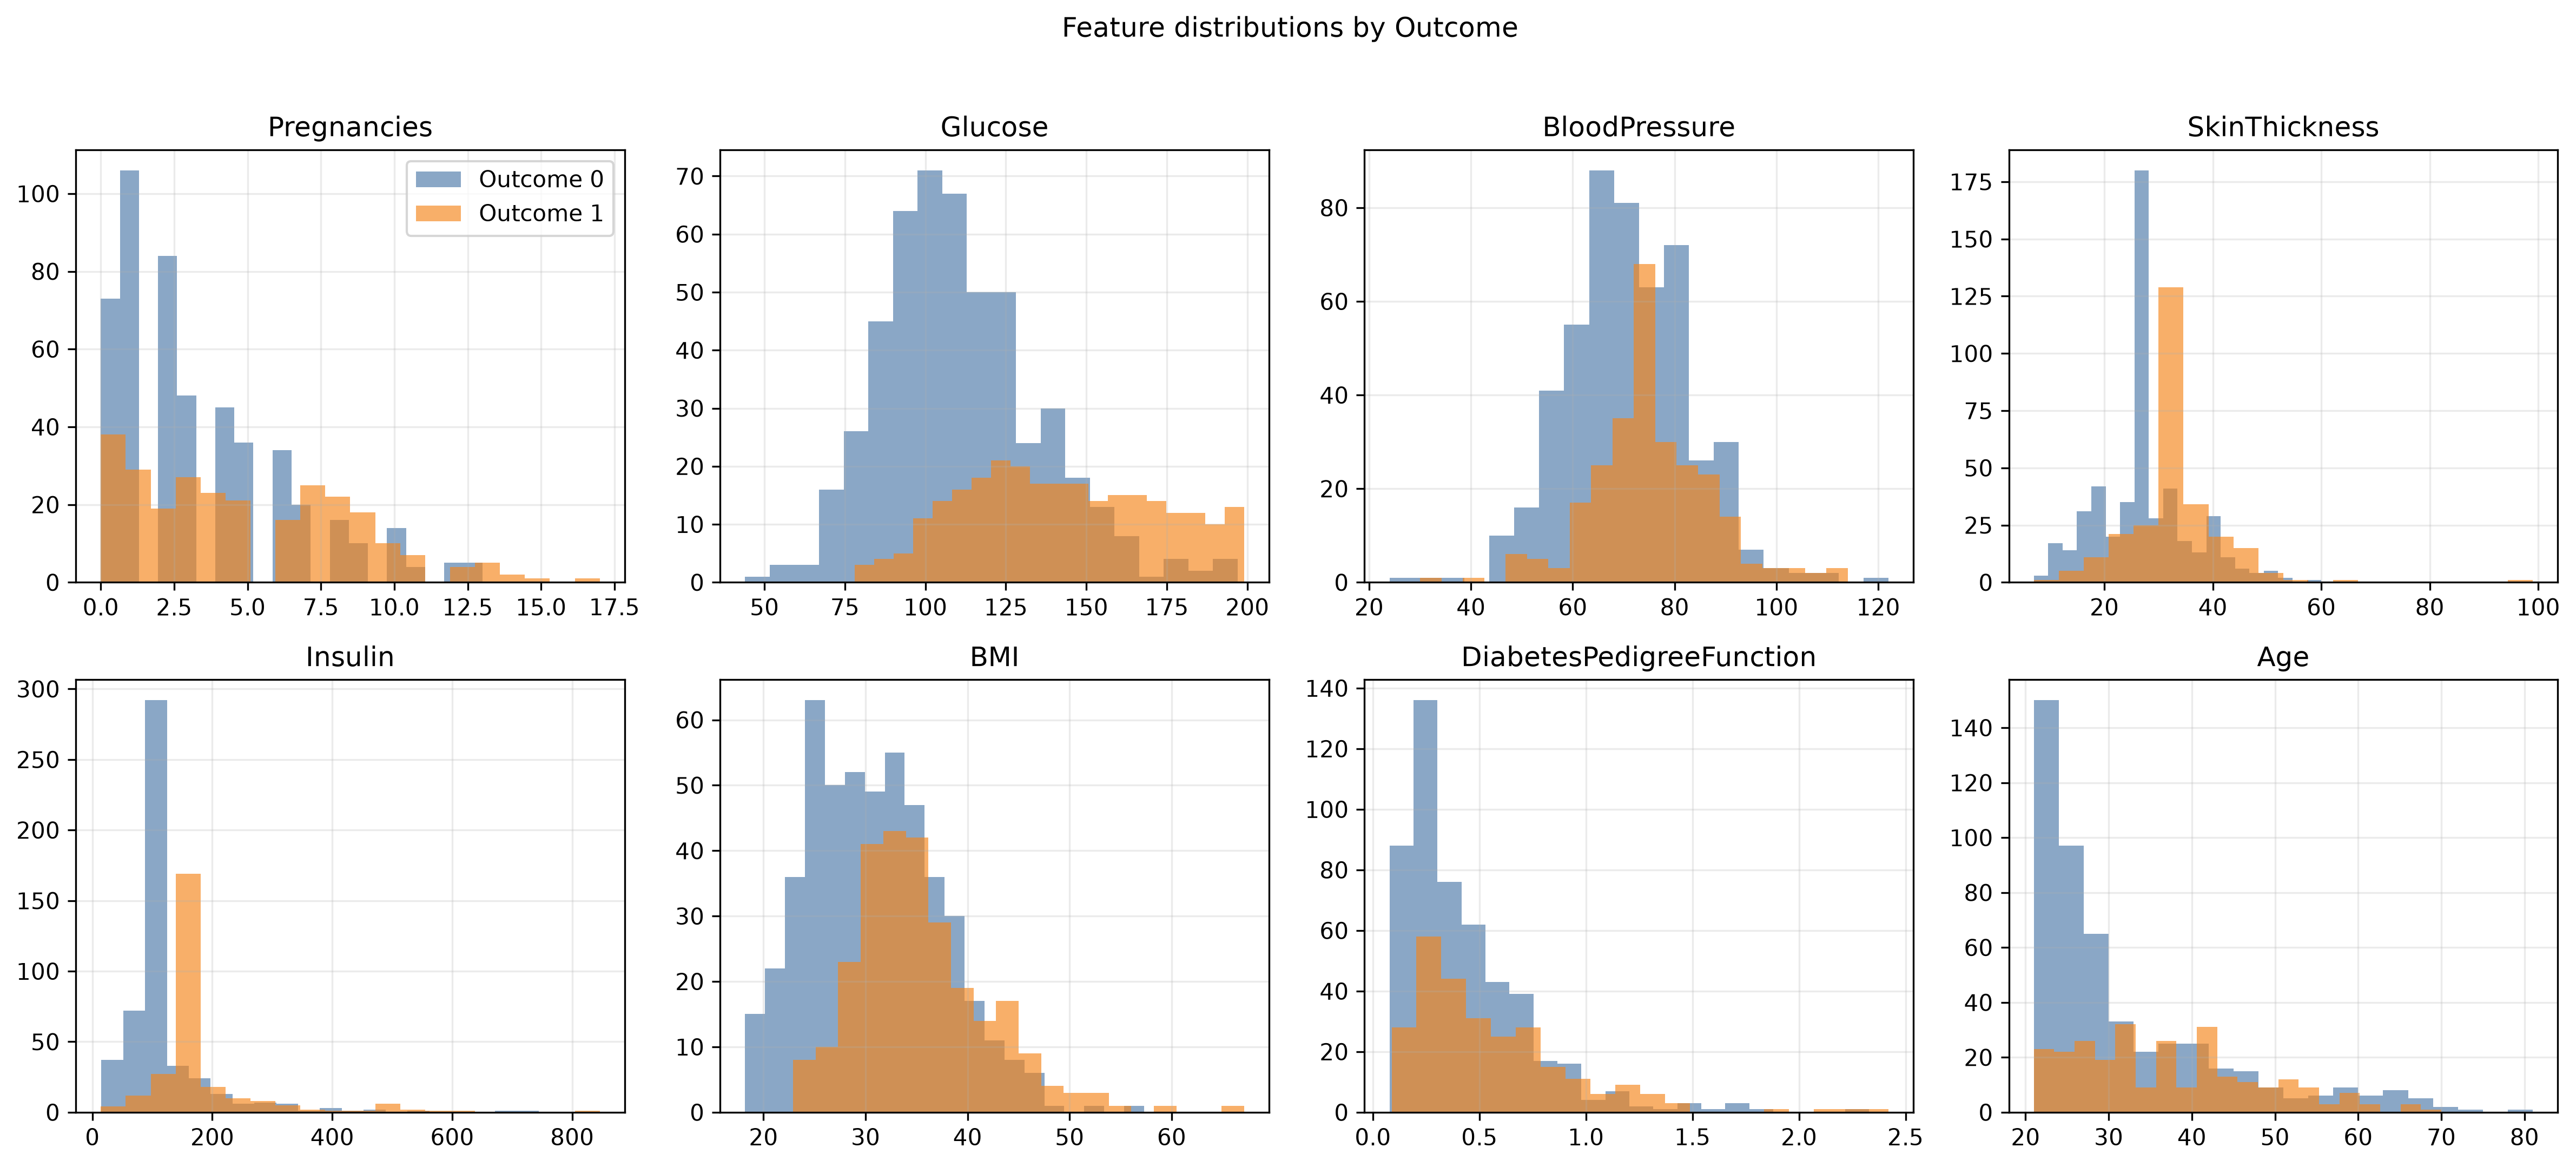
\includegraphics[width=\textwidth]{diabetes_raw_feature_distributions_by_outcome.png}
    \caption{Phân phối các đặc trưng y sinh theo nhãn Outcome}
    \label{fig:diabetes_feature_distribution}
\end{figure}

\begin{figure}[H]
    \centering
    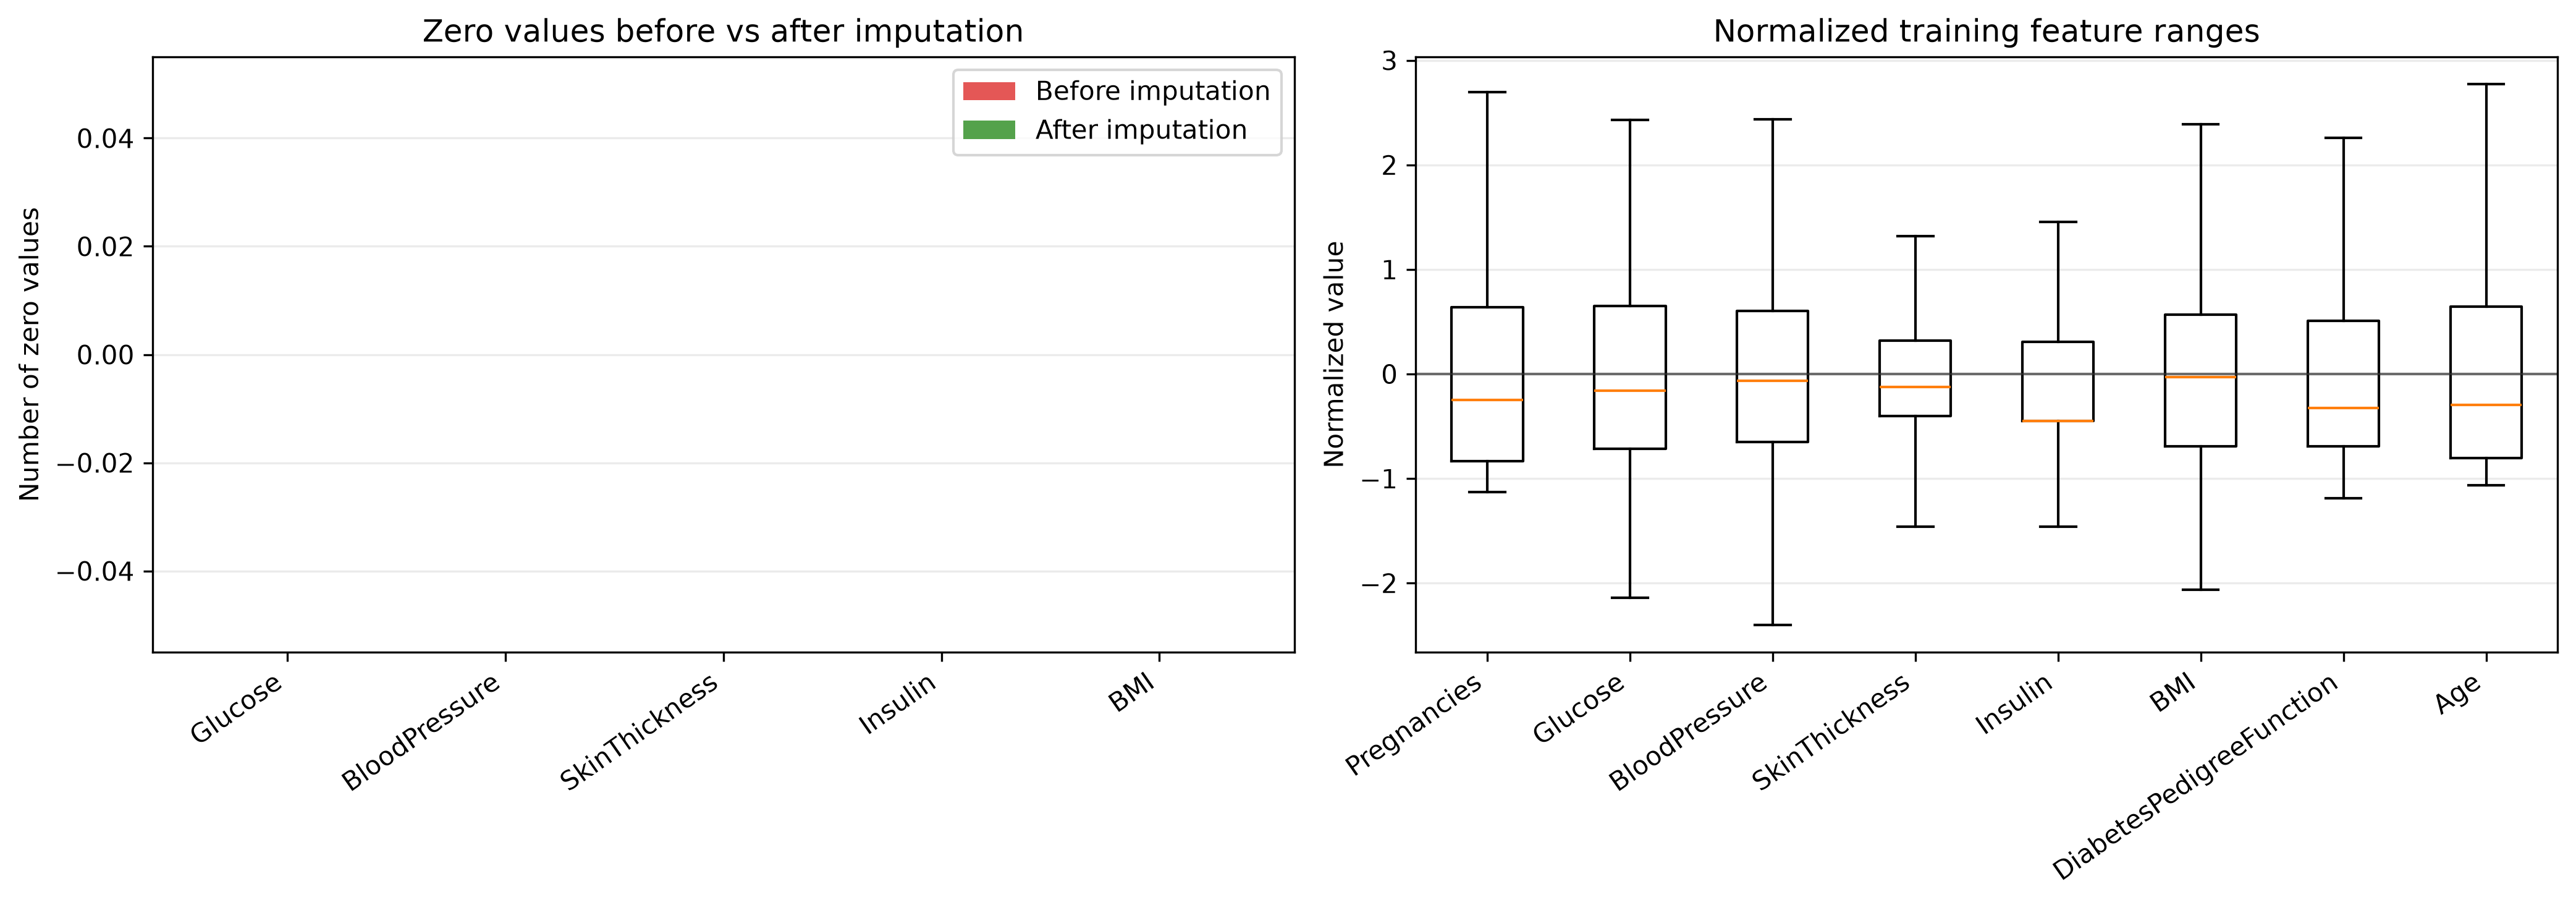
\includegraphics[width=0.95\textwidth]{diabetes_preprocessing_effect.png}
    \caption{Tác động của tiền xử lý: thay thế giá trị 0 bất thường và chuẩn hóa}
    \label{fig:diabetes_preprocessing}
\end{figure}

\section{Cấu hình huấn luyện MLP NumPy}
Phiên bản cải tiến sử dụng kiến trúc MLP nhiều tầng, ReLU ở tầng ẩn, sigmoid ở tầng ra, Binary Cross-Entropy và cập nhật gradient bằng NumPy. So với baseline, notebook bổ sung validation set và early stopping nhằm giảm overfitting.

\subsection{So sánh baseline và phiên bản cải tiến}
Baseline ban đầu có vai trò chứng minh rằng MLP thuần NumPy có thể học được từ dữ liệu diabetes.
Tuy nhiên, baseline còn thiếu một số thành phần thường thấy trong một pipeline thực nghiệm hoàn chỉnh: xử lý missing hợp lý, validation tracking, early stopping và threshold tuning.
Phiên bản cải tiến không thay đổi mục tiêu cốt lõi là tự viết mạng nơ-ron bằng NumPy, nhưng làm cho thực nghiệm gần hơn với cách đánh giá mô hình trong thực tế.

Các cải tiến chính gồm:
\begin{itemize}
    \item Xử lý giá trị 0 bất thường trước khi scale.
    \item Tách validation set để theo dõi loss và accuracy ngoài train.
    \item Dùng early stopping để tránh huấn luyện quá lâu khi validation không còn cải thiện.
    \item Tối ưu threshold theo validation F1 thay vì mặc định 0.5.
\end{itemize}

\subsection{Theo dõi learning curve}
Learning curve trong Hình \ref{fig:diabetes_training_history} cho thấy mô hình không chỉ được đánh giá ở một epoch cuối cùng.
Khi train loss giảm nhưng validation loss tăng, đó là dấu hiệu overfitting.
Khi cả train và validation cùng đi ngang, tiếp tục tăng epoch thường không tạo thêm lợi ích đáng kể.
Do đó early stopping là cách biến quá trình huấn luyện từ ``chạy đủ số vòng'' thành ``dừng khi bằng chứng validation không còn ủng hộ''.

\begin{figure}[H]
    \centering
    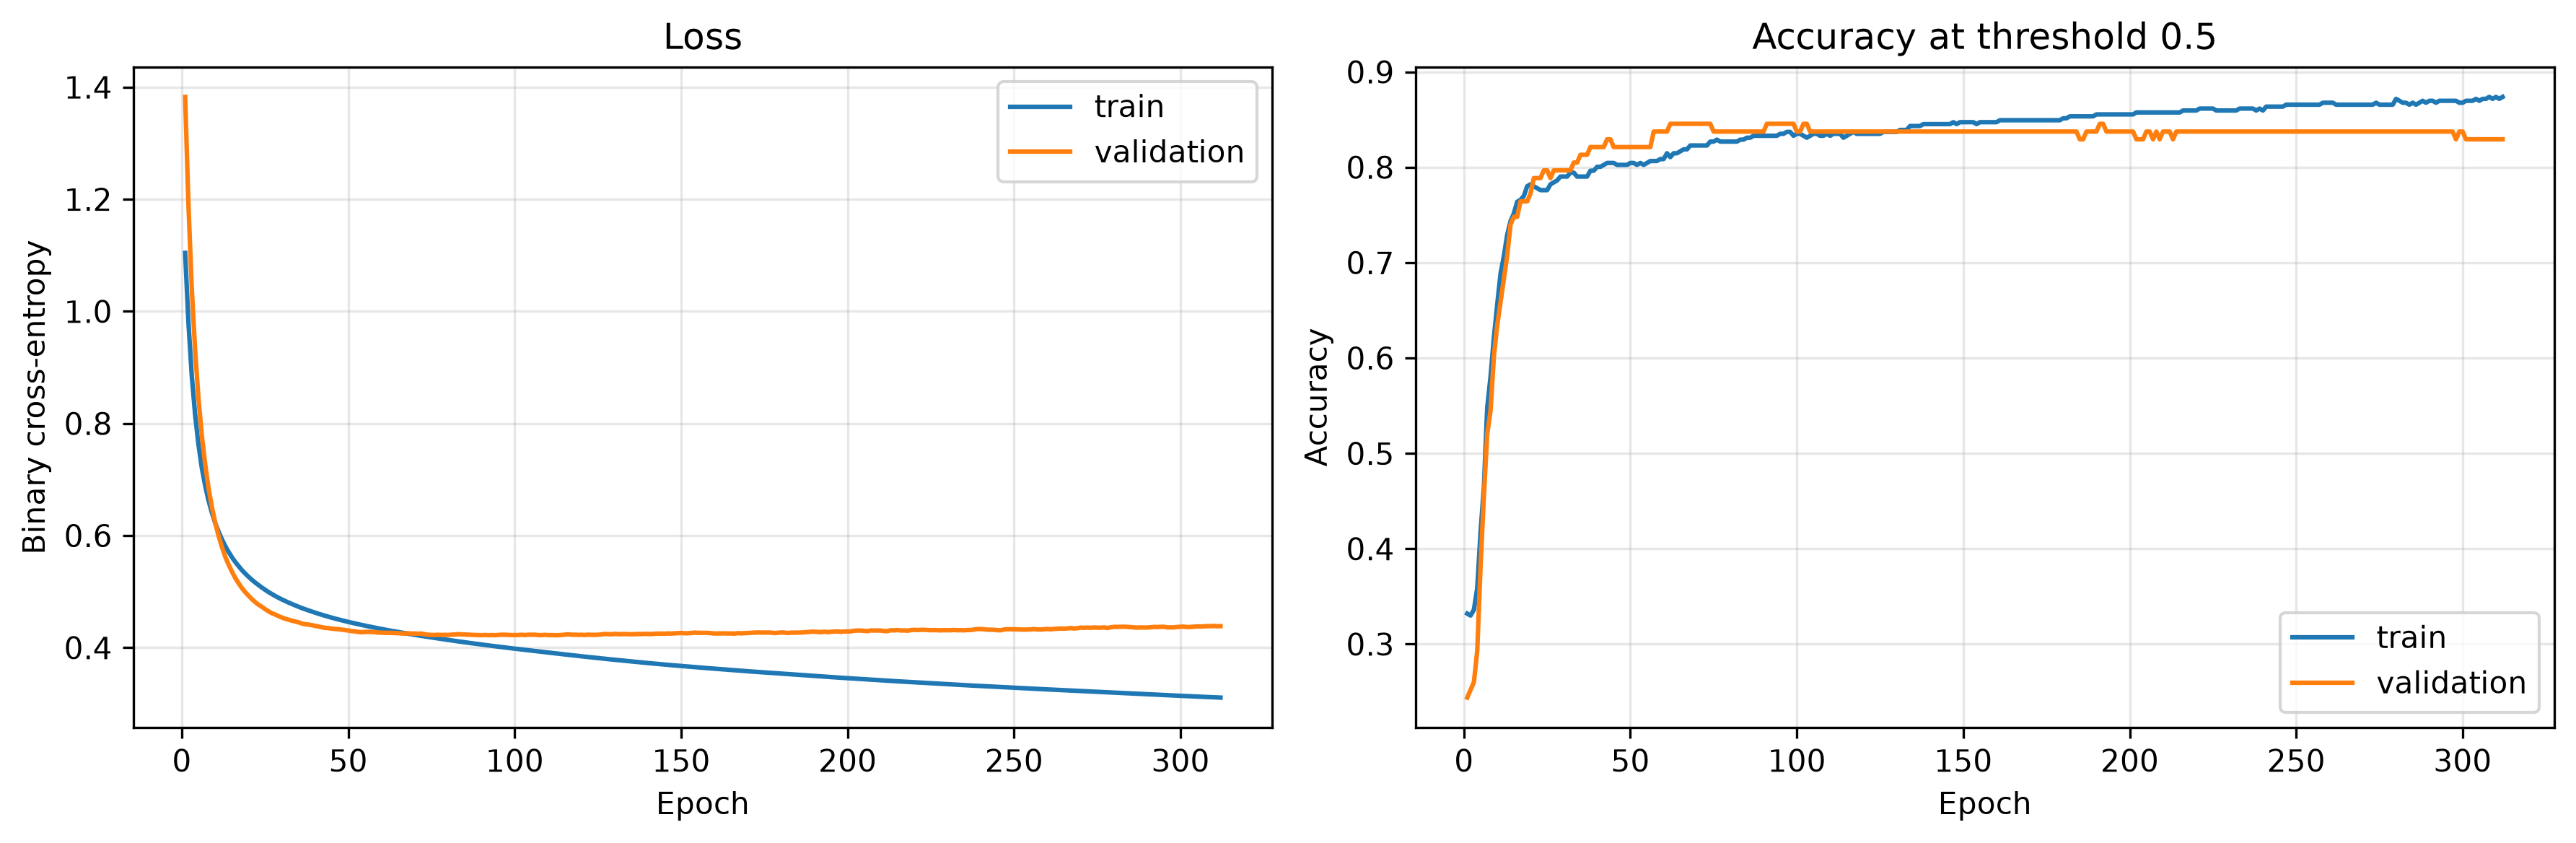
\includegraphics[width=0.95\textwidth]{diabetes_training_history.png}
    \caption{Đường cong loss và accuracy của MLP cải tiến}
    \label{fig:diabetes_training_history}
\end{figure}

\section{Đối chiếu kết quả}
Baseline trong notebook gốc đạt accuracy khoảng 0.7662 trên test set. Phiên bản cải tiến đạt accuracy 0.8571 và F1 0.8308 tại ngưỡng 0.5. Khi chọn ngưỡng tốt nhất trên validation set, test F1 tăng lên 0.8358, recall đạt 0.9655 và số false negative giảm còn 2 ca.

\subsection{Tại sao threshold tuning quan trọng}
Trong phân loại y tế, false negative thường nguy hiểm hơn false positive vì bệnh nhân có nguy cơ bị bỏ sót.
Ngưỡng 0.5 không phản ánh trực tiếp chi phí sai lỗi này.
Khi giảm ngưỡng xuống 0.47, mô hình dự đoán nhiều mẫu dương hơn, từ đó recall tăng lên 0.9655.
Precision có thể giảm nhẹ, nhưng F1 vẫn tăng vì cân bằng tổng thể giữa precision và recall tốt hơn.

\begin{lstlisting}[language=Python, caption={Minh họa chọn threshold theo validation F1}, label={lst:threshold}]
best_threshold = 0.5
best_f1 = -1.0

for threshold in np.linspace(0.05, 0.95, 91):
    y_val_pred = (y_val_proba >= threshold).astype(int)
    score = f1_score(y_val, y_val_pred)

    if score > best_f1:
        best_f1 = score
        best_threshold = threshold

y_test_pred = (y_test_proba >= best_threshold).astype(int)
\end{lstlisting}

\subsection{Diễn giải kết quả diabetes nhỏ}
Kết quả ở Bảng \ref{tab:diabetes_small_results} cho thấy cải tiến pipeline tạo khác biệt rõ so với baseline.
Accuracy tăng từ 0.7662 lên 0.8571.
Quan trọng hơn, recall ở threshold đã chọn đạt 0.9655, nghĩa là phần lớn mẫu bệnh được phát hiện.
Trong bối cảnh sàng lọc y tế, đây là hướng ưu tiên hợp lý hơn so với chỉ tối đa hóa accuracy.

Tuy vậy, kết quả cũng cần được đọc với sự thận trọng.
Dataset chỉ có 768 mẫu, vì vậy một vài dự đoán khác đi có thể làm metric thay đổi đáng kể.
Báo cáo do đó xem diabetes nhỏ như một thực nghiệm nền, còn kết luận so sánh mô hình toàn diện hơn được đặt ở các chương tiếp theo với dữ liệu lớn và đa dạng hơn.

\begin{table}[H]
\centering
\caption{So sánh baseline và MLP cải tiến trên bộ Diabetes}
\label{tab:diabetes_small_results}
\begin{tabular}{lcccc}
\toprule
\textbf{Mô hình} & \textbf{Threshold} & \textbf{Accuracy} & \textbf{Recall} & \textbf{F1} \\
\midrule
Baseline NumPy MLP & 0.50 & 0.7662 & -- & -- \\
Improved MLP & 0.50 & 0.8571 & 0.9310 & 0.8308 \\
Improved MLP & 0.47 & 0.8571 & \textbf{0.9655} & \textbf{0.8358} \\
\bottomrule
\end{tabular}
\end{table}

\begin{figure}[H]
    \centering
    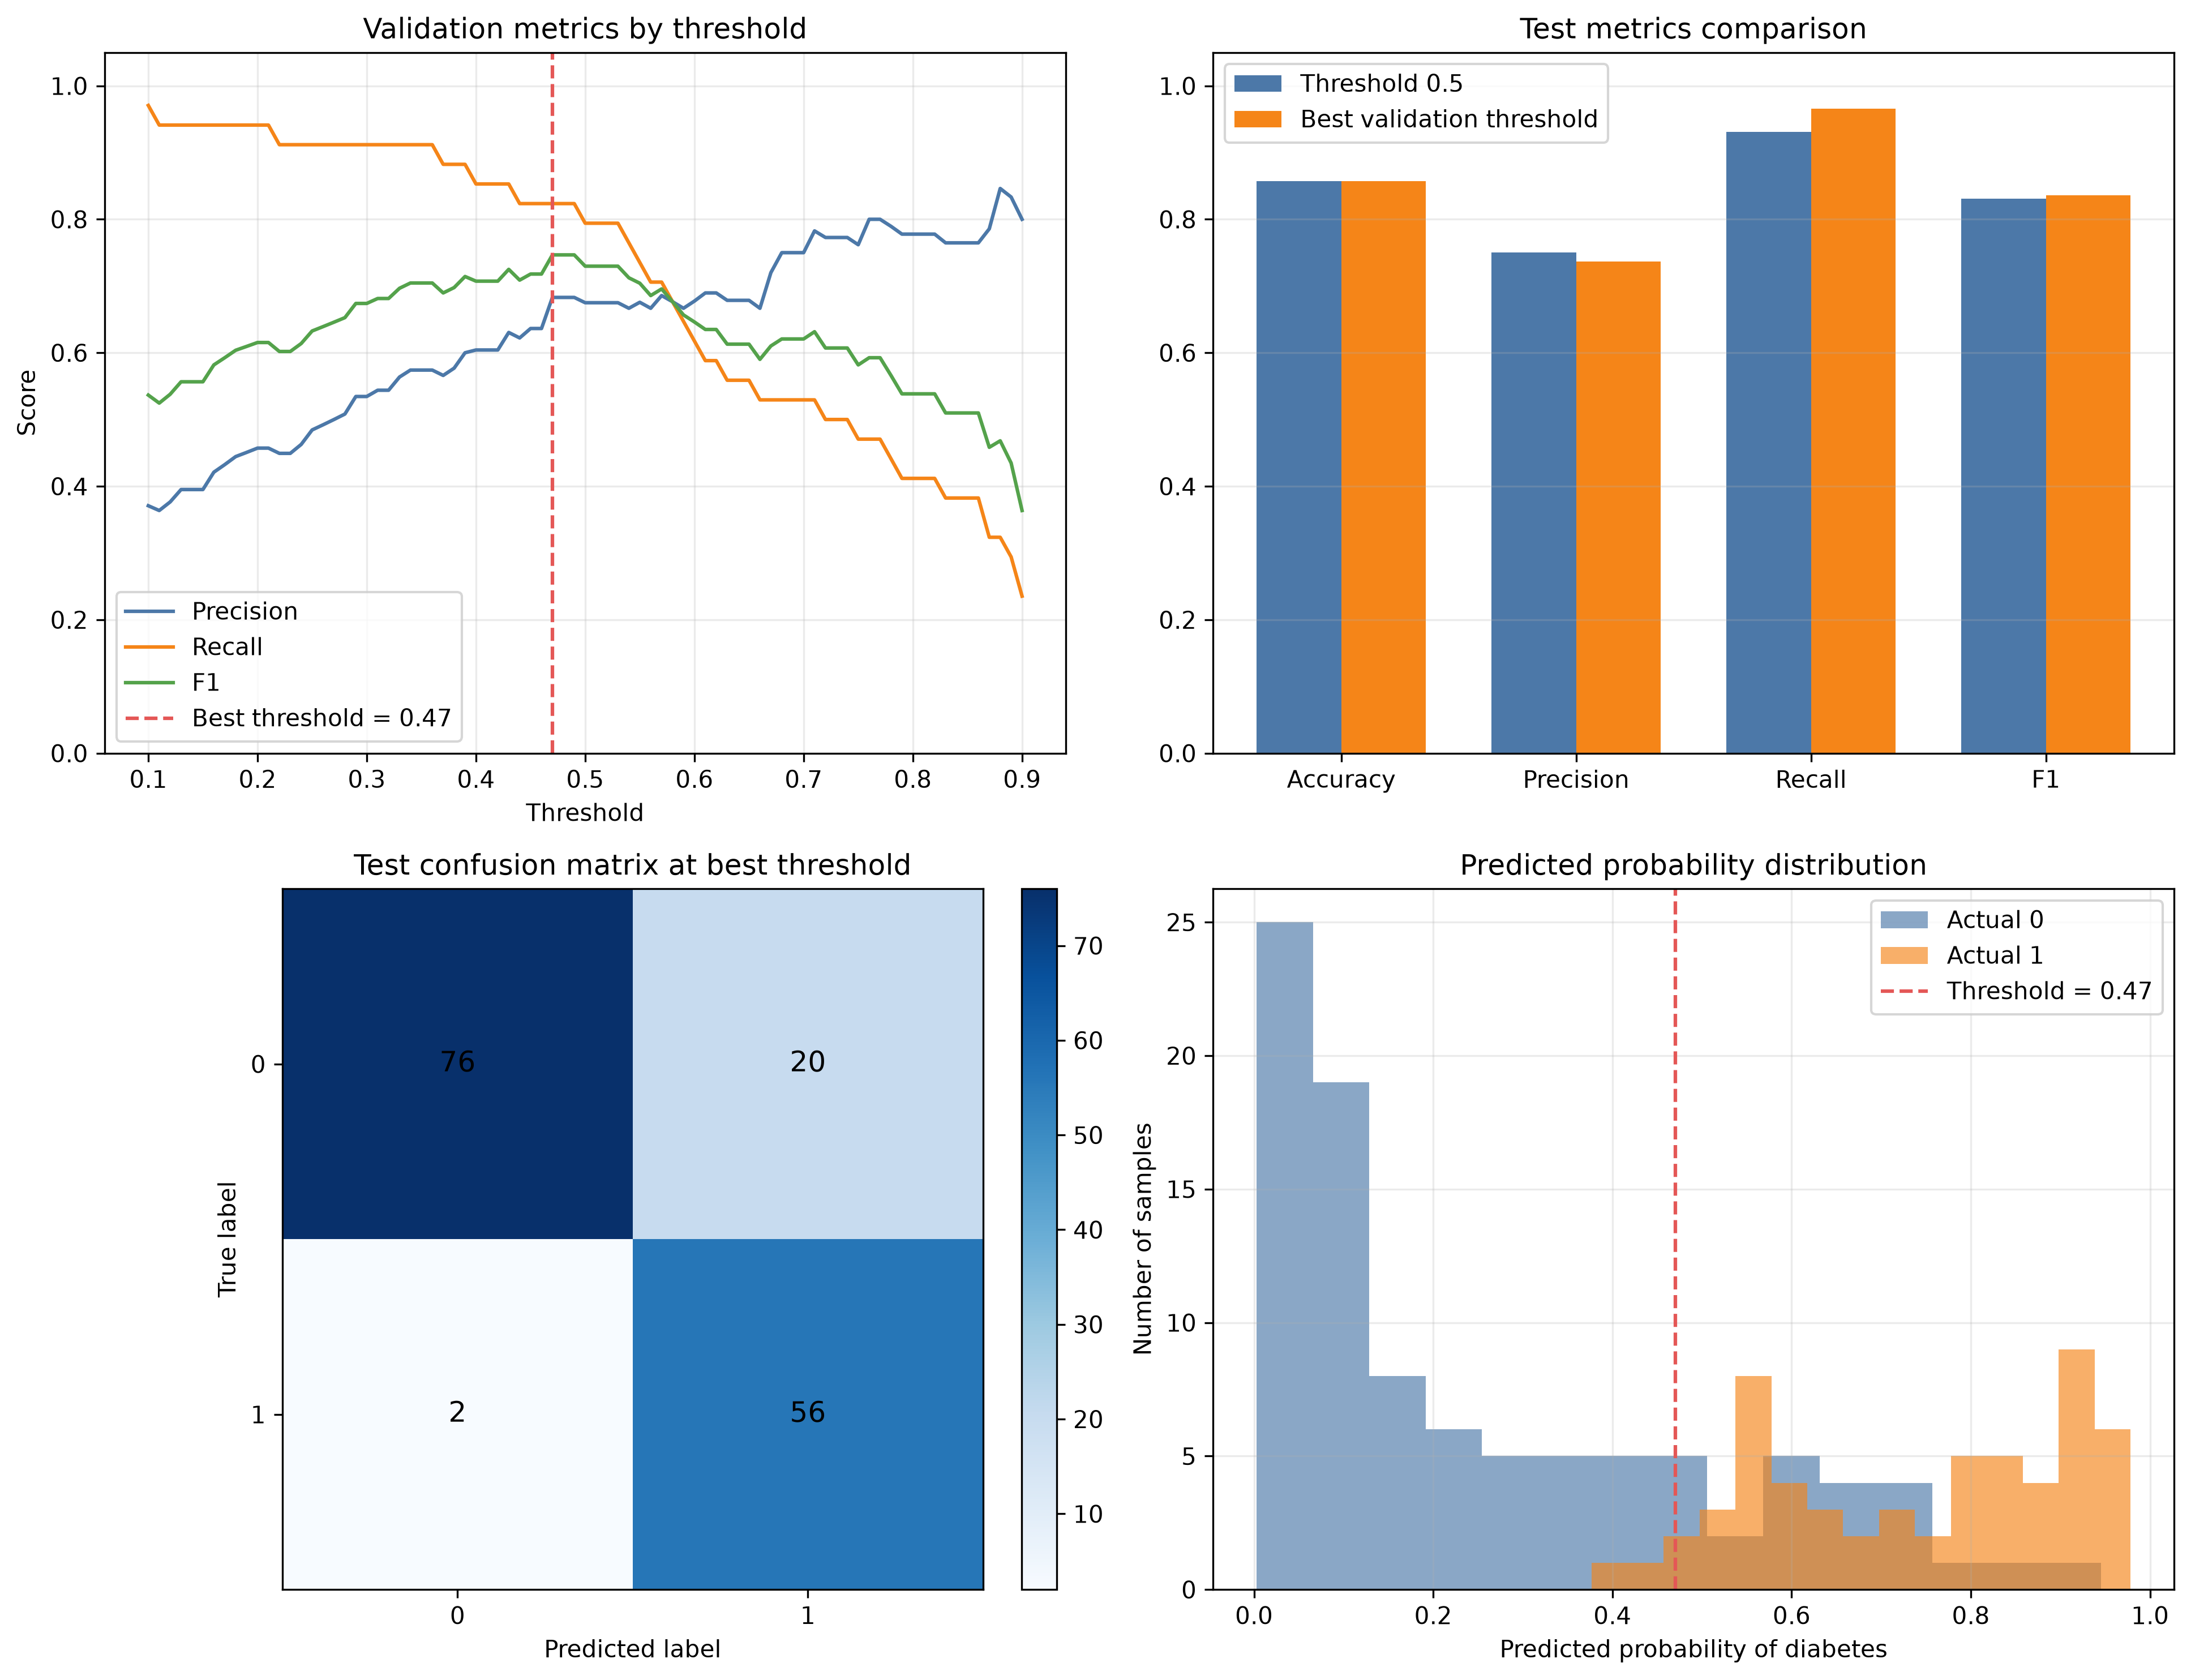
\includegraphics[width=\textwidth]{diabetes_evaluation_results.png}
    \caption{Threshold tuning, metric comparison, confusion matrix và phân phối xác suất dự đoán}
    \label{fig:diabetes_evaluation}
\end{figure}

% =========================================================================
% CHUONG 3
% =========================================================================
\chapter{Diabetes Large: Đối Chuẩn Trên Dữ Liệu Mất Cân Bằng}

\section{Dữ liệu và mục tiêu đánh giá}
Notebook \modelpath{Assignment3/diabetes\_large/notebook/diabetes\_large\_benchmark.ipynb} xử lý bài toán phân loại tiểu đường trên 100,000 mẫu. Dataset có các cột số như \texttt{age}, \texttt{bmi}, \texttt{HbA1c\_level}, \texttt{blood\_glucose\_level} và cột phân loại như \texttt{gender}, \texttt{smoking\_history}. Nhãn \texttt{diabetes} có tỷ lệ dương khoảng 8.5\%, do đó notebook đánh giá thêm precision, recall, F1, ROC-AUC và PR-AUC bên cạnh accuracy.

\subsection{Đặc thù dữ liệu mất cân bằng}
Tỷ lệ dương khoảng 8.5\% nghĩa là một mô hình luôn dự đoán ``không tiểu đường'' vẫn có thể đạt accuracy xấp xỉ 91.5\%.
Con số này nhìn qua có vẻ cao nhưng hoàn toàn vô dụng cho mục tiêu phát hiện bệnh.
Vì vậy chương này ưu tiên F1 và PR-AUC.
F1 buộc mô hình cân bằng giữa precision và recall, còn PR-AUC cho biết chất lượng xếp hạng của mô hình trong vùng lớp dương hiếm.

\subsection{Tín hiệu y sinh trong feature}
Các feature \texttt{HbA1c\_level} và \texttt{blood\_glucose\_level} thường là tín hiệu mạnh vì liên quan trực tiếp đến chẩn đoán tiểu đường.
Tuy nhiên mô hình vẫn cần các feature khác như tuổi, BMI, tiền sử hút thuốc, huyết áp và bệnh tim để nắm bắt rủi ro tổng hợp.
Decision Tree có lợi thế khi dữ liệu có các ngưỡng tách tự nhiên.
Logistic Regression lại phù hợp khi quan hệ giữa feature đã xử lý và log-odds của nhãn gần tuyến tính.

\section{Khảo sát và biến đổi đặc trưng}
Notebook dùng one-hot encoding cho biến phân loại, chuẩn hóa biến số và chia train/validation/test theo stratified split 70/15/15. Tất cả scaler/encoder chỉ được fit trên training set nhằm chống rò rỉ dữ liệu.

\subsection{One-hot encoding và chuẩn hóa}
Hai cột \texttt{gender} và \texttt{smoking\_history} được one-hot encode để đưa về dạng số.
Các cột số được scale để Logistic Regression và MLP hội tụ ổn định hơn.
Gaussian Naive Bayes không bắt buộc scale về mặt lý thuyết, nhưng vẫn được đánh giá trên cùng không gian feature để benchmark công bằng.
Decision Tree ít nhạy với thang đo, song dùng chung pipeline giúp kết quả giữa các mô hình không bị lệch do khác tiền xử lý.

\subsection{Class weighting trong huấn luyện}
Với lớp dương hiếm, loss bình thường có thể bị lớp âm chi phối.
Class weighting tăng trọng số của mẫu dương trong quá trình tính loss và gradient.
Trong MLP NumPy, ý tưởng này được hiện thực bằng cách nhân sai số từng mẫu với trọng số tương ứng.
Trong scikit-learn, Logistic Regression và Decision Tree dùng tham số \texttt{class\_weight='balanced'} để đạt mục tiêu tương tự.

\begin{figure}[H]
    \centering
    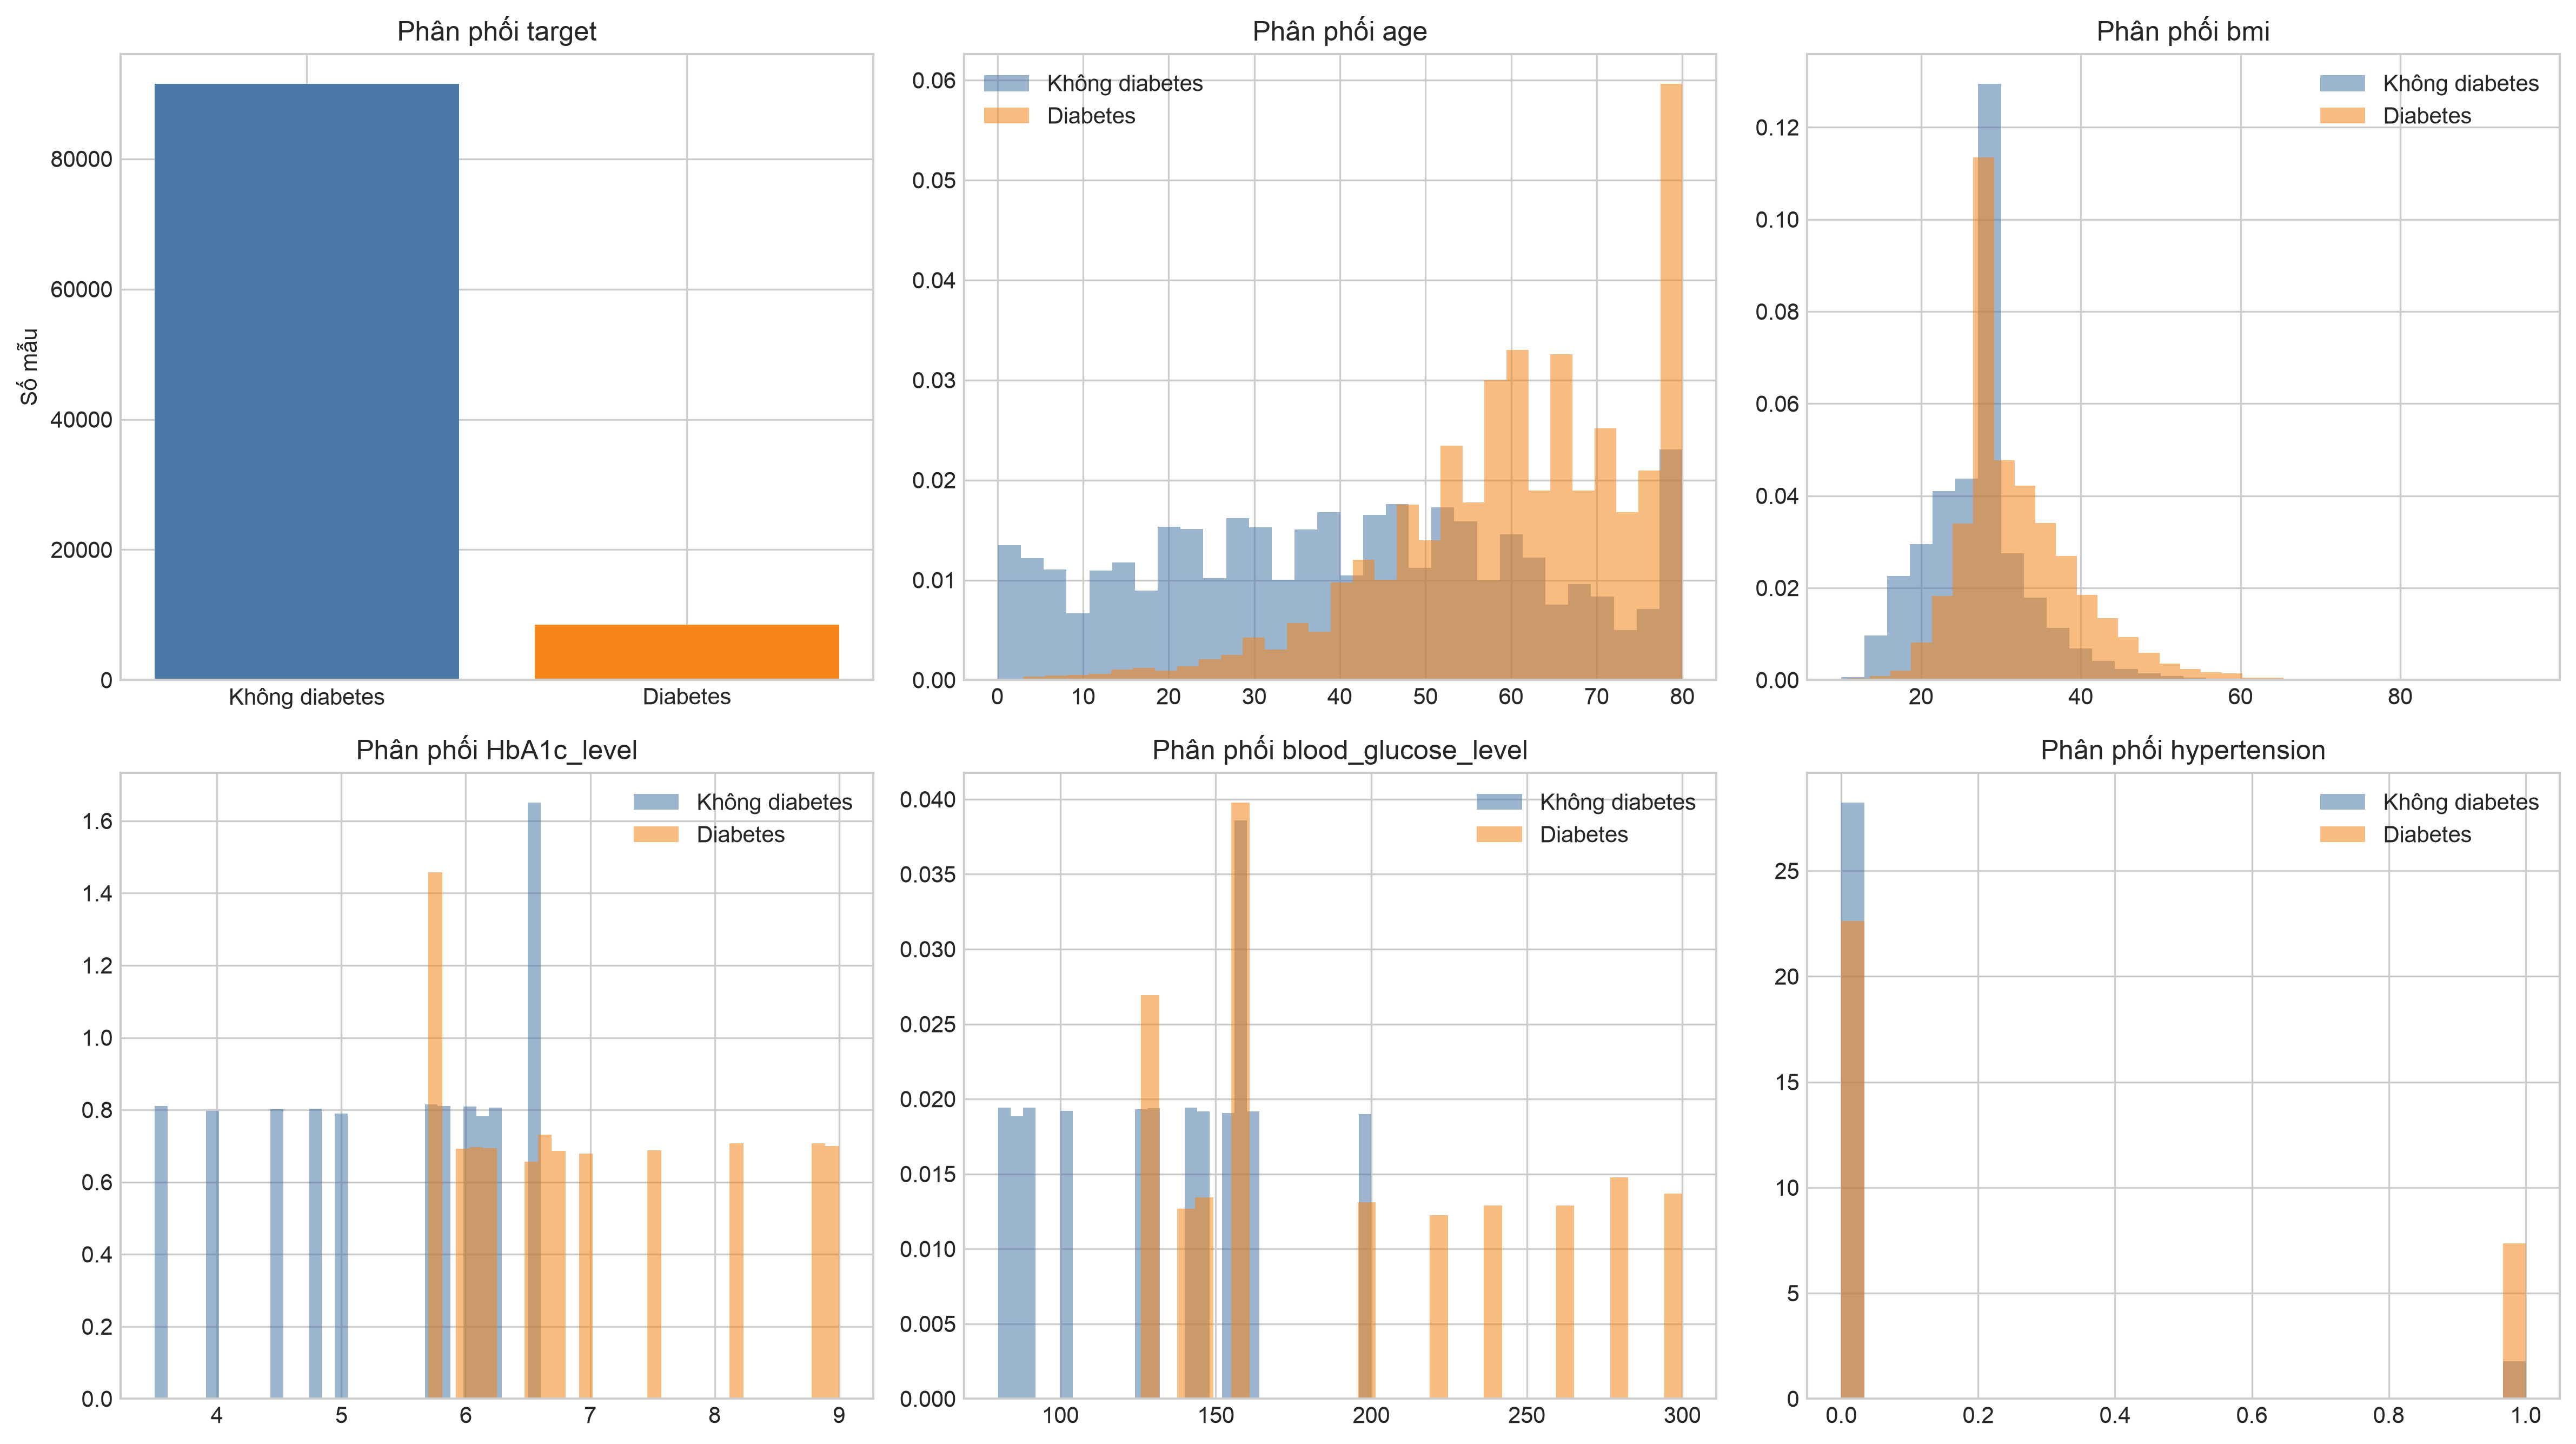
\includegraphics[width=\textwidth]{diabetes_large_eda_numeric_distributions.png}
    \caption{Phân phối các đặc trưng số chính theo nhãn diabetes}
    \label{fig:diabetes_large_numeric}
\end{figure}

\begin{figure}[H]
    \centering
    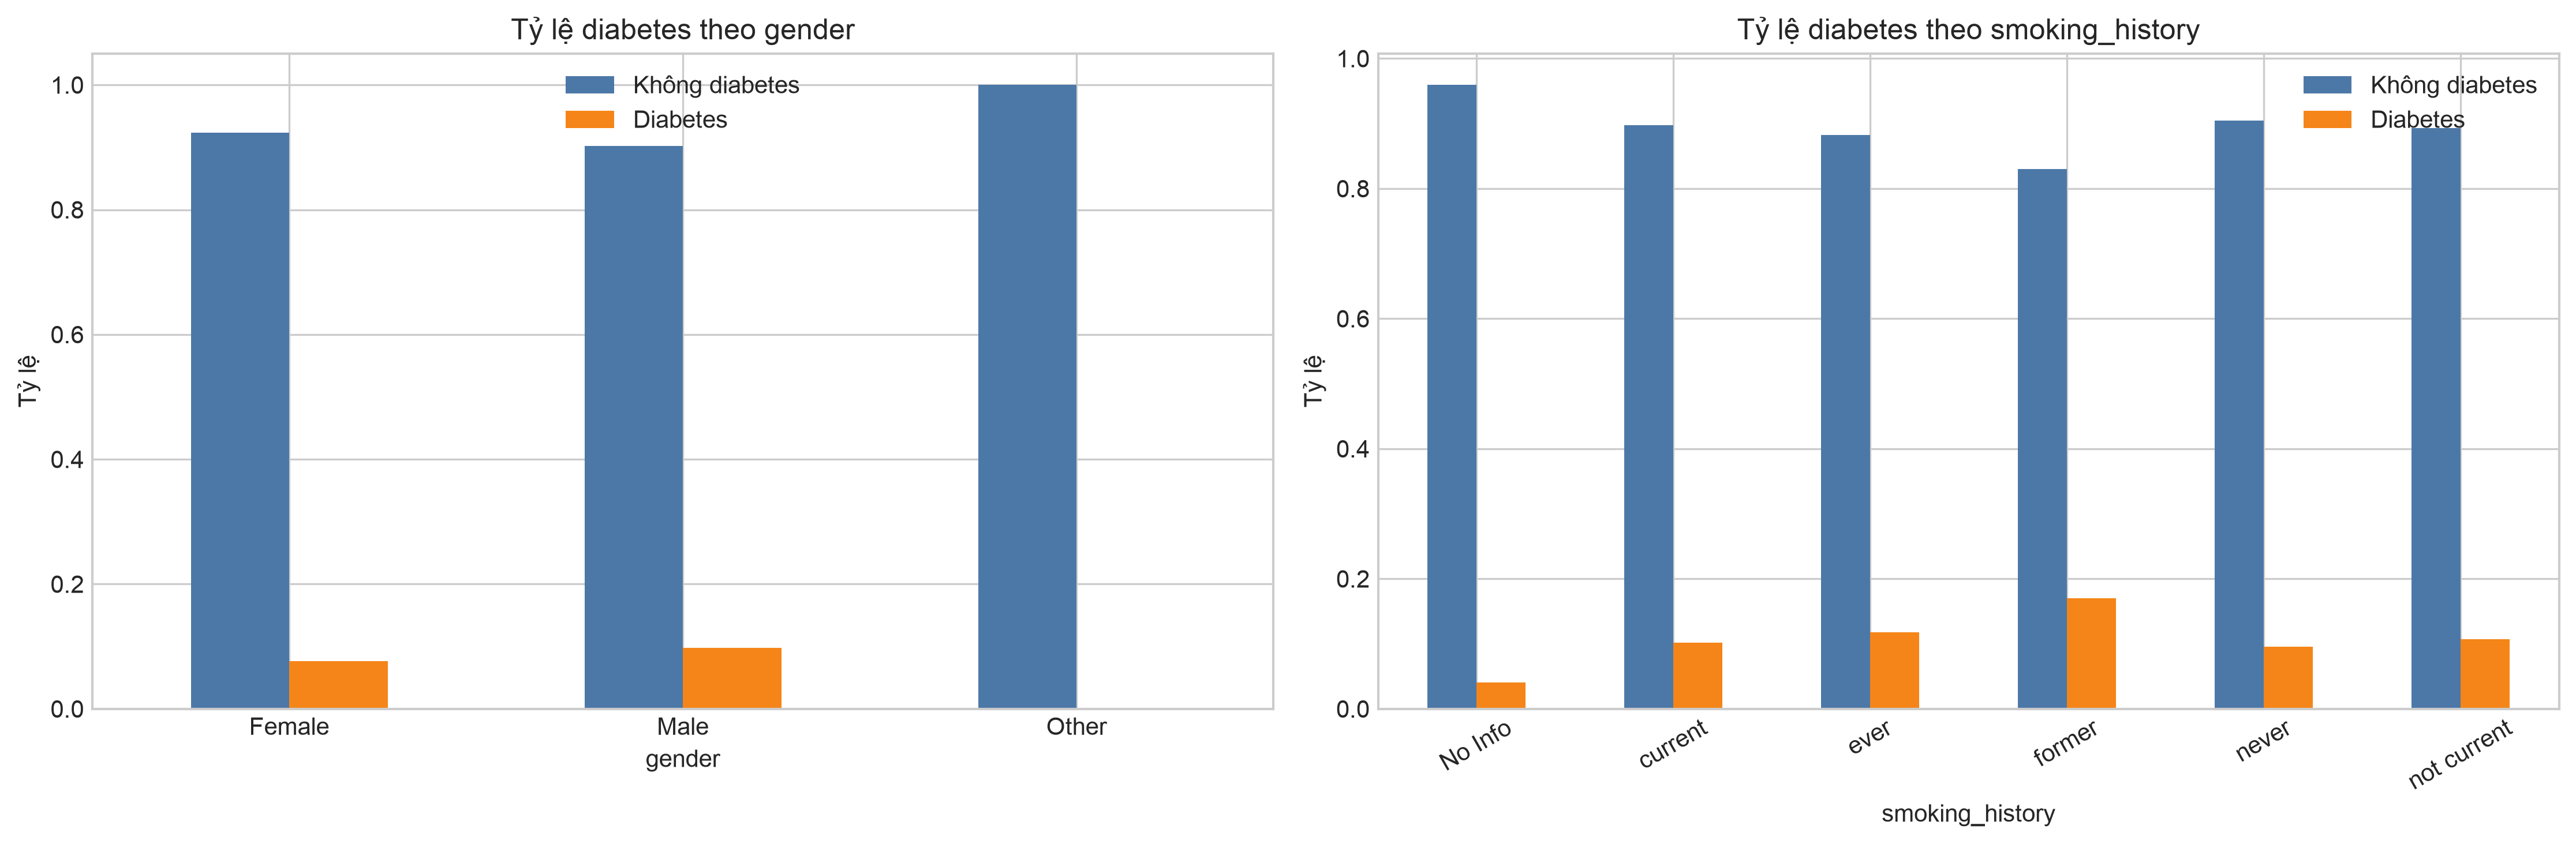
\includegraphics[width=\textwidth]{diabetes_large_eda_categorical_rates.png}
    \caption{Tỷ lệ diabetes theo gender và smoking history}
    \label{fig:diabetes_large_categorical}
\end{figure}

\section{Các mô hình trong benchmark}
Bốn mô hình được huấn luyện trên cùng pipeline:
\begin{itemize}
    \item Logistic Regression với class weight balanced.
    \item Gaussian Naive Bayes.
    \item Decision Tree với class weight balanced.
    \item MLP thuần NumPy kiến trúc $input \to 64 \to 32 \to 16 \to 1$.
\end{itemize}
MLP dùng ReLU, sigmoid, mini-batch gradient descent, class weighting, L2 regularization và early stopping theo validation PR-AUC.

\subsection{Phân tích từng mô hình}
Logistic Regression là baseline tuyến tính mạnh.
Ưu điểm của mô hình này là huấn luyện nhanh, dễ giải thích và thường hoạt động tốt khi feature đã được chuẩn hóa.
Kết quả F1 0.7300 và PR-AUC 0.8209 cho thấy baseline tuyến tính đã khai thác được phần lớn tín hiệu của dữ liệu.

Gaussian Naive Bayes đạt recall cao nhất 0.8376 nhưng precision chỉ 0.3083.
Điều này có nghĩa mô hình phát hiện được nhiều ca dương, nhưng đồng thời tạo nhiều cảnh báo dương sai.
Kết quả phù hợp với giả định độc lập feature của Naive Bayes: giả định này đơn giản, nhanh, nhưng không đủ chặt cho dữ liệu y sinh có nhiều tương quan.

Decision Tree đạt F1 và PR-AUC cao nhất.
Lợi thế chính là mô hình có thể học các quy tắc dạng ngưỡng, ví dụ khi chỉ số đường huyết hoặc HbA1c vượt một mức nào đó.
Tuy nhiên tree đơn cũng có nguy cơ overfit nếu không giới hạn độ sâu.
Notebook vì vậy dùng cấu hình kiểm soát độ phức tạp và đánh giá trên test set tách riêng.

MLP NumPy đạt ROC-AUC 0.9658 và PR-AUC 0.8265, gần với Logistic Regression và Decision Tree.
Điểm đáng chú ý là mô hình học bằng NumPy thuần vẫn cạnh tranh trên dữ liệu 100,000 mẫu.
Chi phí huấn luyện cao hơn nhiều so với các mô hình scikit-learn, nhưng đổi lại báo cáo kiểm soát rõ từng bước forward, backward, regularization và early stopping.

\begin{figure}[H]
    \centering
    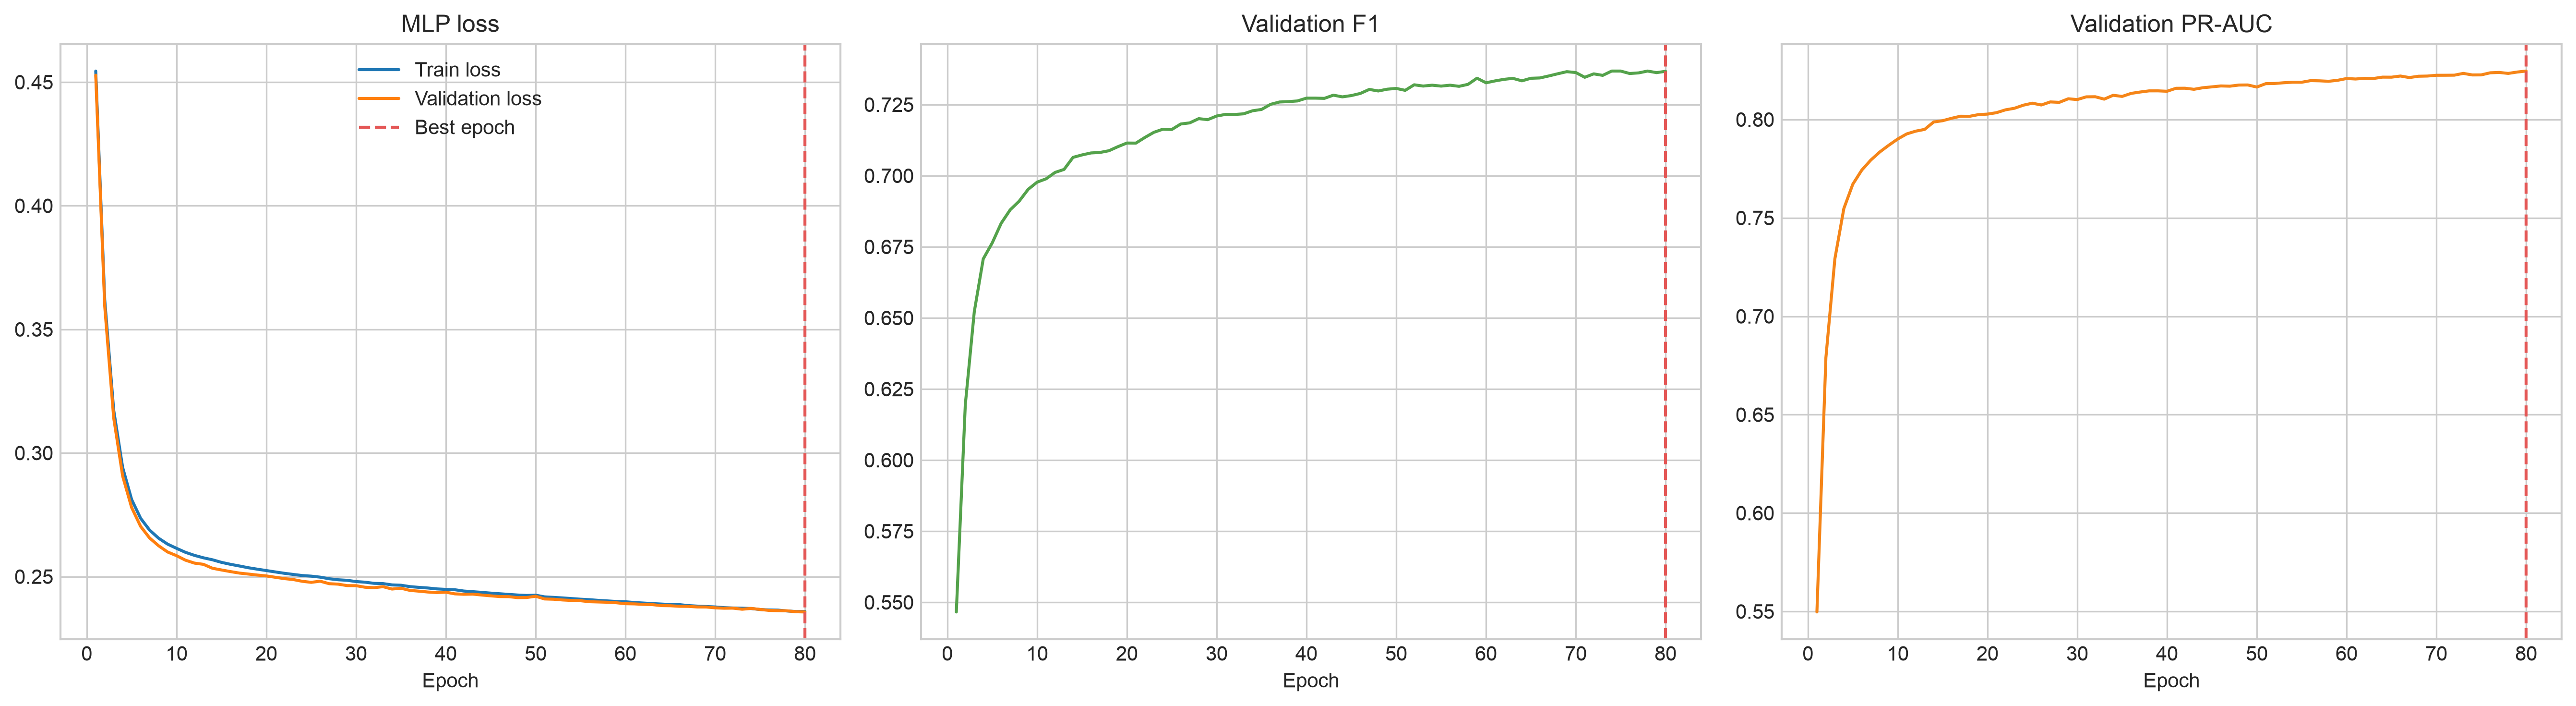
\includegraphics[width=0.95\textwidth]{diabetes_large_mlp_learning_curve.png}
    \caption{Learning curve của MLP NumPy trên diabetes large}
    \label{fig:diabetes_large_learning_curve}
\end{figure}

\section{Kết quả trên tập test}
Decision Tree đạt kết quả tốt nhất theo F1 và PR-AUC trên test set. MLP NumPy có ROC-AUC cao, nhưng F1 thấp hơn Decision Tree do precision/recall trade-off trên dữ liệu mất cân bằng.

\subsection{Đọc bảng kết quả theo nhiều trục}
Nếu chỉ nhìn accuracy, Decision Tree cũng đứng đầu với 0.9721.
Tuy nhiên lý do chọn Decision Tree không chỉ nằm ở accuracy mà nằm ở F1 0.8039 và PR-AUC 0.8514.
Precision 1.0000 cho thấy tại threshold đã chọn, các ca được dự đoán dương đều là dương thật trong test set.
Đổi lại recall 0.6722 thấp hơn Gaussian Naive Bayes, nghĩa là vẫn còn một phần ca dương bị bỏ sót.

Trong ứng dụng y tế thực tế, lựa chọn mô hình còn phụ thuộc chi phí nghiệp vụ.
Nếu mục tiêu là sàng lọc rộng, có thể chấp nhận Gaussian Naive Bayes hoặc một threshold thấp hơn để tăng recall.
Nếu mục tiêu là khuyến nghị kiểm tra chuyên sâu với chi phí cao, precision cao của Decision Tree hấp dẫn hơn.
Báo cáo vì vậy kết luận theo F1/PR-AUC, nhưng vẫn giữ lại toàn bộ metric để người đọc hiểu trade-off.

\begin{table}[H]
\centering
\caption{Benchmark 4 mô hình trên diabetes large}
\label{tab:diabetes_large_benchmark}
\resizebox{\textwidth}{!}{%
\begin{tabular}{lcccccccc}
\toprule
\textbf{Mô hình} & \textbf{Threshold} & \textbf{Accuracy} & \textbf{Precision} & \textbf{Recall} & \textbf{F1} & \textbf{ROC-AUC} & \textbf{PR-AUC} & \textbf{Train(s)} \\
\midrule
Decision Tree & 0.890 & \textbf{0.9721} & \textbf{1.0000} & 0.6722 & \textbf{0.8039} & \textbf{0.9731} & \textbf{0.8514} & 0.0635 \\
NumPy MLP (64-32-16) & 0.845 & 0.9559 & 0.7593 & 0.7051 & 0.7312 & 0.9658 & 0.8265 & 17.2372 \\
Logistic Regression & 0.875 & 0.9573 & 0.7900 & 0.6784 & 0.7300 & 0.9629 & 0.8209 & 0.0341 \\
Gaussian Naive Bayes & 0.950 & 0.8265 & 0.3083 & \textbf{0.8376} & 0.4507 & 0.9093 & 0.5043 & \textbf{0.0087} \\
\bottomrule
\end{tabular}%
}
\end{table}

\begin{figure}[H]
    \centering
    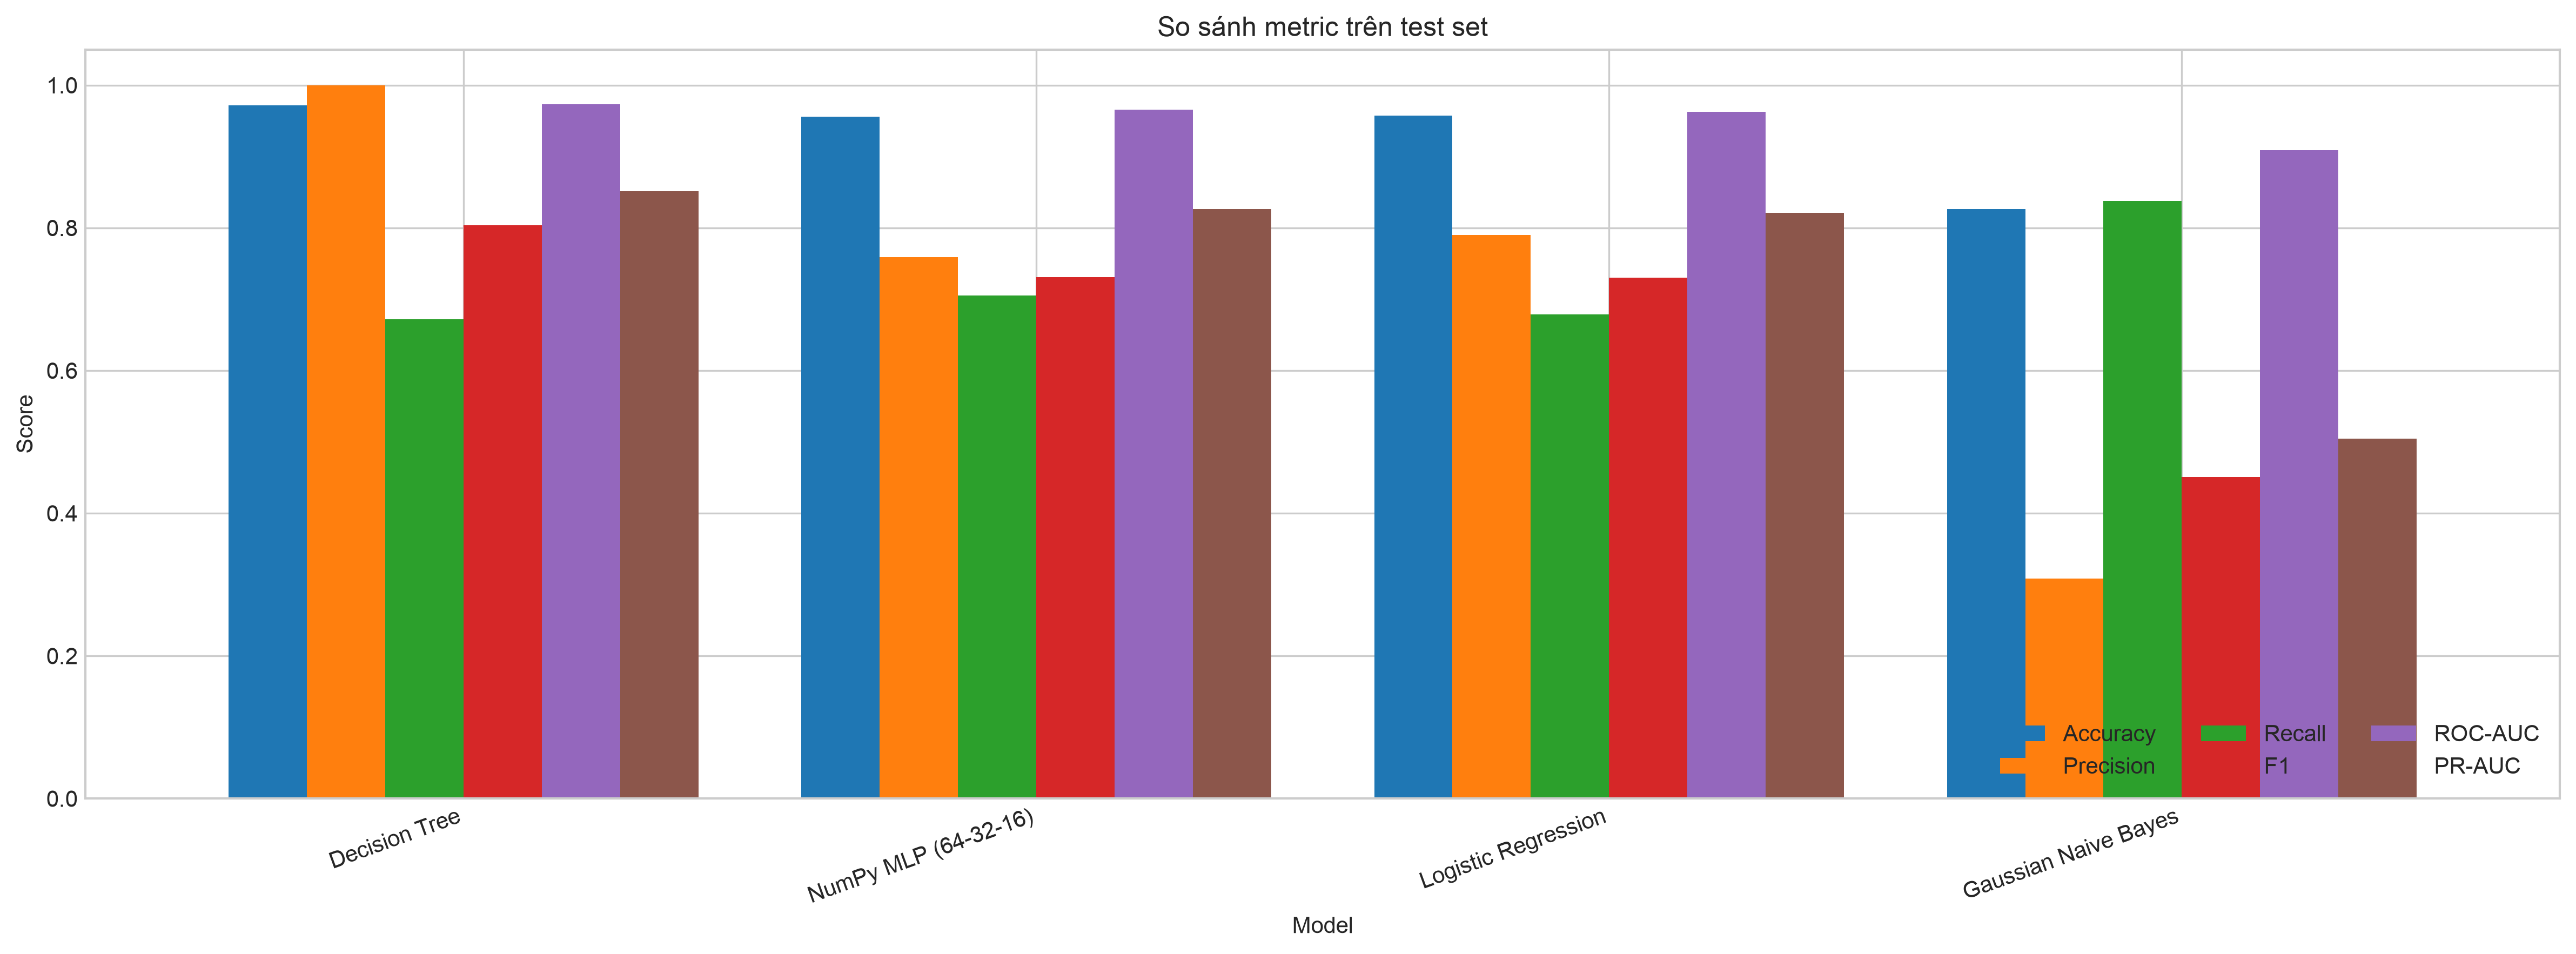
\includegraphics[width=\textwidth]{diabetes_large_metric_comparison.png}
    \caption{So sánh đa chỉ số trên diabetes large}
    \label{fig:diabetes_large_metric_comparison}
\end{figure}

\begin{figure}[H]
    \centering
    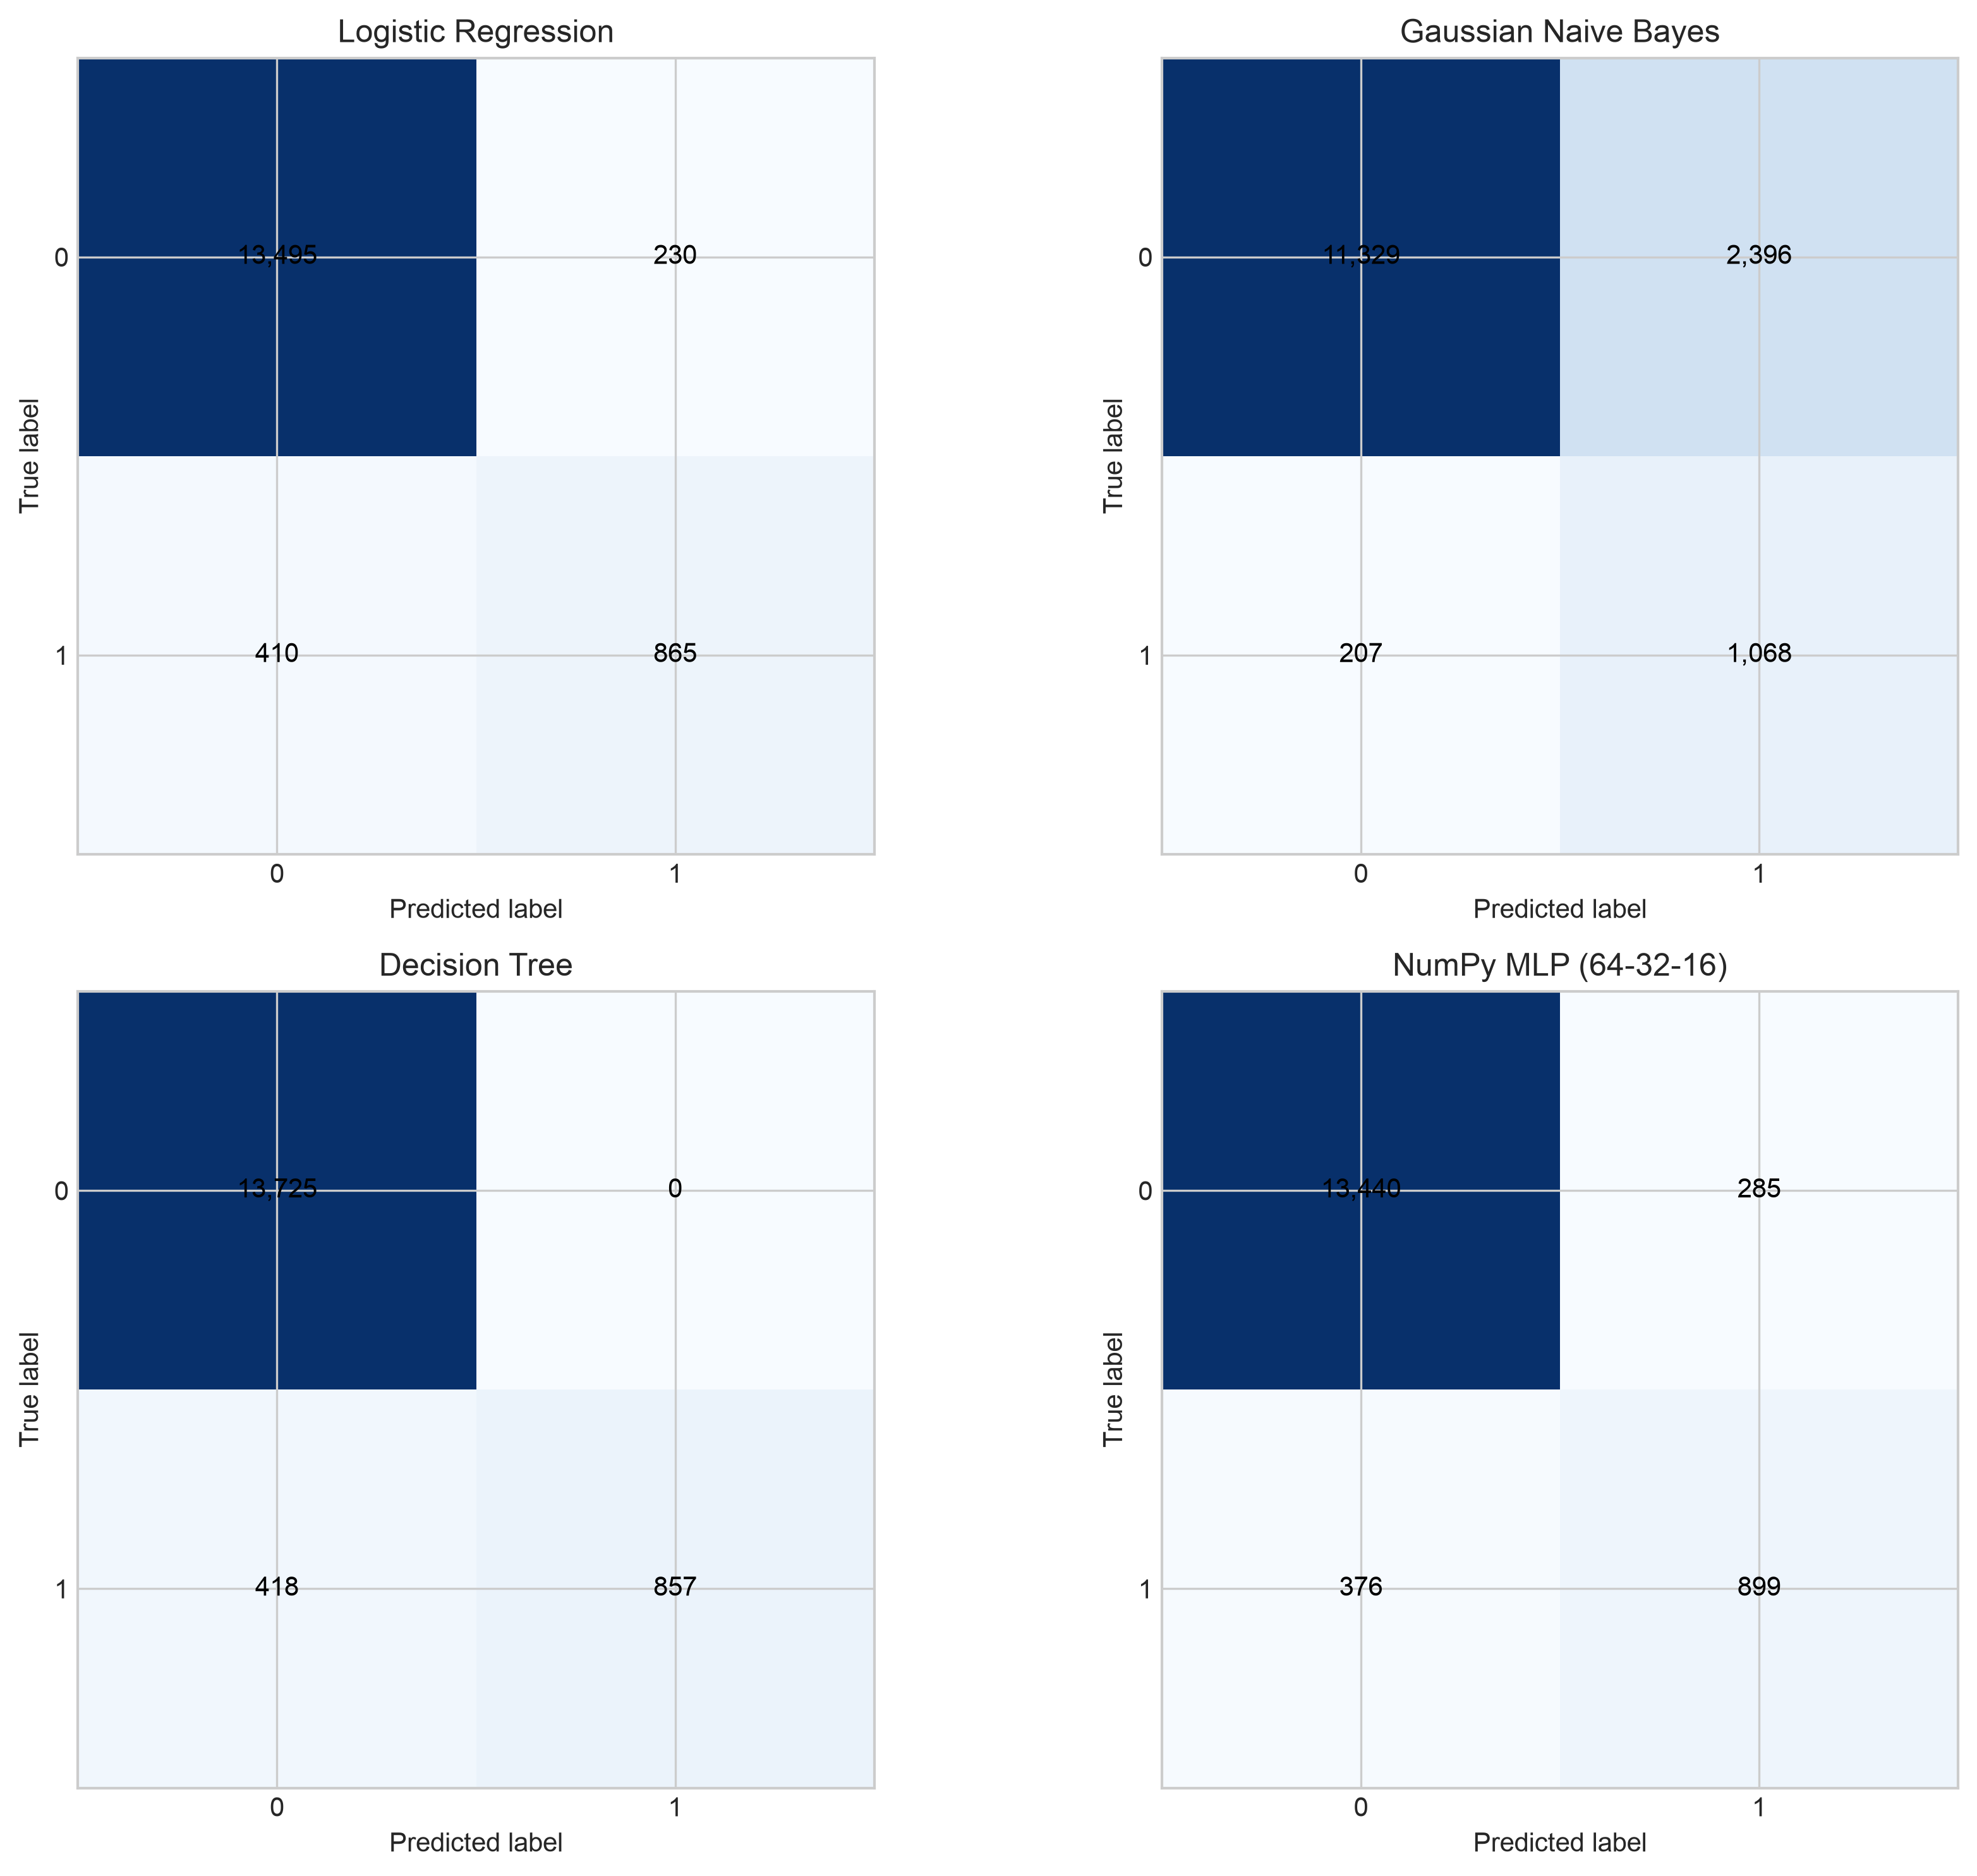
\includegraphics[width=\textwidth]{diabetes_large_confusion_matrices.png}
    \caption{Ma trận nhầm lẫn của 4 mô hình diabetes large}
    \label{fig:diabetes_large_confusion}
\end{figure}

% =========================================================================
% CHUONG 4
% =========================================================================
\chapter{House Price: Hồi Quy Trên Thang Logarit}

\section{Dữ liệu và biến mục tiêu}
Notebook \modelpath{Assignment3/house\_price/notebook/house\_price\_benchmark.ipynb} xử lý bài toán hồi quy giá nhà từ dataset \modelpath{realtor-data.zip.csv}. Dataset được đọc trong notebook có 2,226,382 dòng; sau bước lọc và lấy mẫu với \texttt{RANDOM\_STATE = 42}, tập dùng cho mô hình gồm 200,000 dòng.

Target \texttt{price} có phân phối lệch mạnh và chứa nhiều outlier giá cao. Do đó các mô hình được huấn luyện trên $log1p(price)$ rồi chuyển ngược về USD để đánh giá.

\subsection{Vì sao cần log-transform target}
Giá nhà thường có phân phối lệch phải: phần lớn căn nhà nằm ở vùng giá phổ biến, trong khi một số ít căn rất đắt tạo đuôi dài.
Nếu huấn luyện trực tiếp trên USD bằng MSE, các căn giá cực cao sẽ chi phối gradient.
Mô hình có thể cải thiện RMSE bằng cách tập trung vào outlier nhưng lại dự đoán kém ở nhóm nhà phổ biến.

Biến đổi $log1p(price)$ làm nén đuôi phải và biến sai số tuyệt đối lớn thành sai số tương đối dễ quản lý hơn.
Khi đánh giá, notebook chuyển dự đoán về USD bằng $expm1$ để báo cáo MAE, RMSE và MedianAE theo đơn vị gốc.
RMSLE được dùng như metric chính vì nhất quán với cách huấn luyện trên log scale.

\section{Khảo sát dữ liệu và tạo đặc trưng}
Các đặc trưng gồm số phòng ngủ, phòng tắm, diện tích đất, diện tích nhà, trạng thái giao dịch, thành phố, bang, zip code, broker và ngày bán trước. Pipeline thực hiện median imputation, missing indicators, log-transform cho \texttt{acre\_lot}/\texttt{house\_size}, one-hot cho \texttt{status}/\texttt{state}, frequency encoding cho các biến high-cardinality và tách đặc trưng thời gian từ \texttt{prev\_sold\_date}.

\subsection{Feature engineering cho dữ liệu bất động sản}
Bài toán giá nhà phụ thuộc mạnh vào vị trí.
Tuy nhiên các biến như \texttt{city}, \texttt{zip\_code} và \texttt{brokered\_by} có nhiều giá trị khác nhau.
Nếu one-hot toàn bộ, ma trận feature có thể rất rộng và khó huấn luyện bằng MLP NumPy.
Frequency encoding là lựa chọn thực dụng: mỗi giá trị phân loại được thay bằng tần suất xuất hiện của nó trong train set.
Cách này không biểu diễn được thứ tự địa lý thật, nhưng giữ lại thông tin về mức độ phổ biến và giảm mạnh số chiều.

\begin{lstlisting}[language=Python, caption={Minh họa feature engineering cho house price}, label={lst:house_feature_engineering}]
train["log_price"] = np.log1p(train["price"])
train["log_acre_lot"] = np.log1p(train["acre_lot"].clip(lower=0))
train["log_house_size"] = np.log1p(train["house_size"].clip(lower=0))

freq = train["zip_code"].value_counts(normalize=True)
train["zip_code_freq"] = train["zip_code"].map(freq).fillna(0)
test["zip_code_freq"] = test["zip_code"].map(freq).fillna(0)

train["prev_sold_year"] = pd.to_datetime(
    train["prev_sold_date"], errors="coerce"
).dt.year
\end{lstlisting}

\begin{figure}[H]
    \centering
    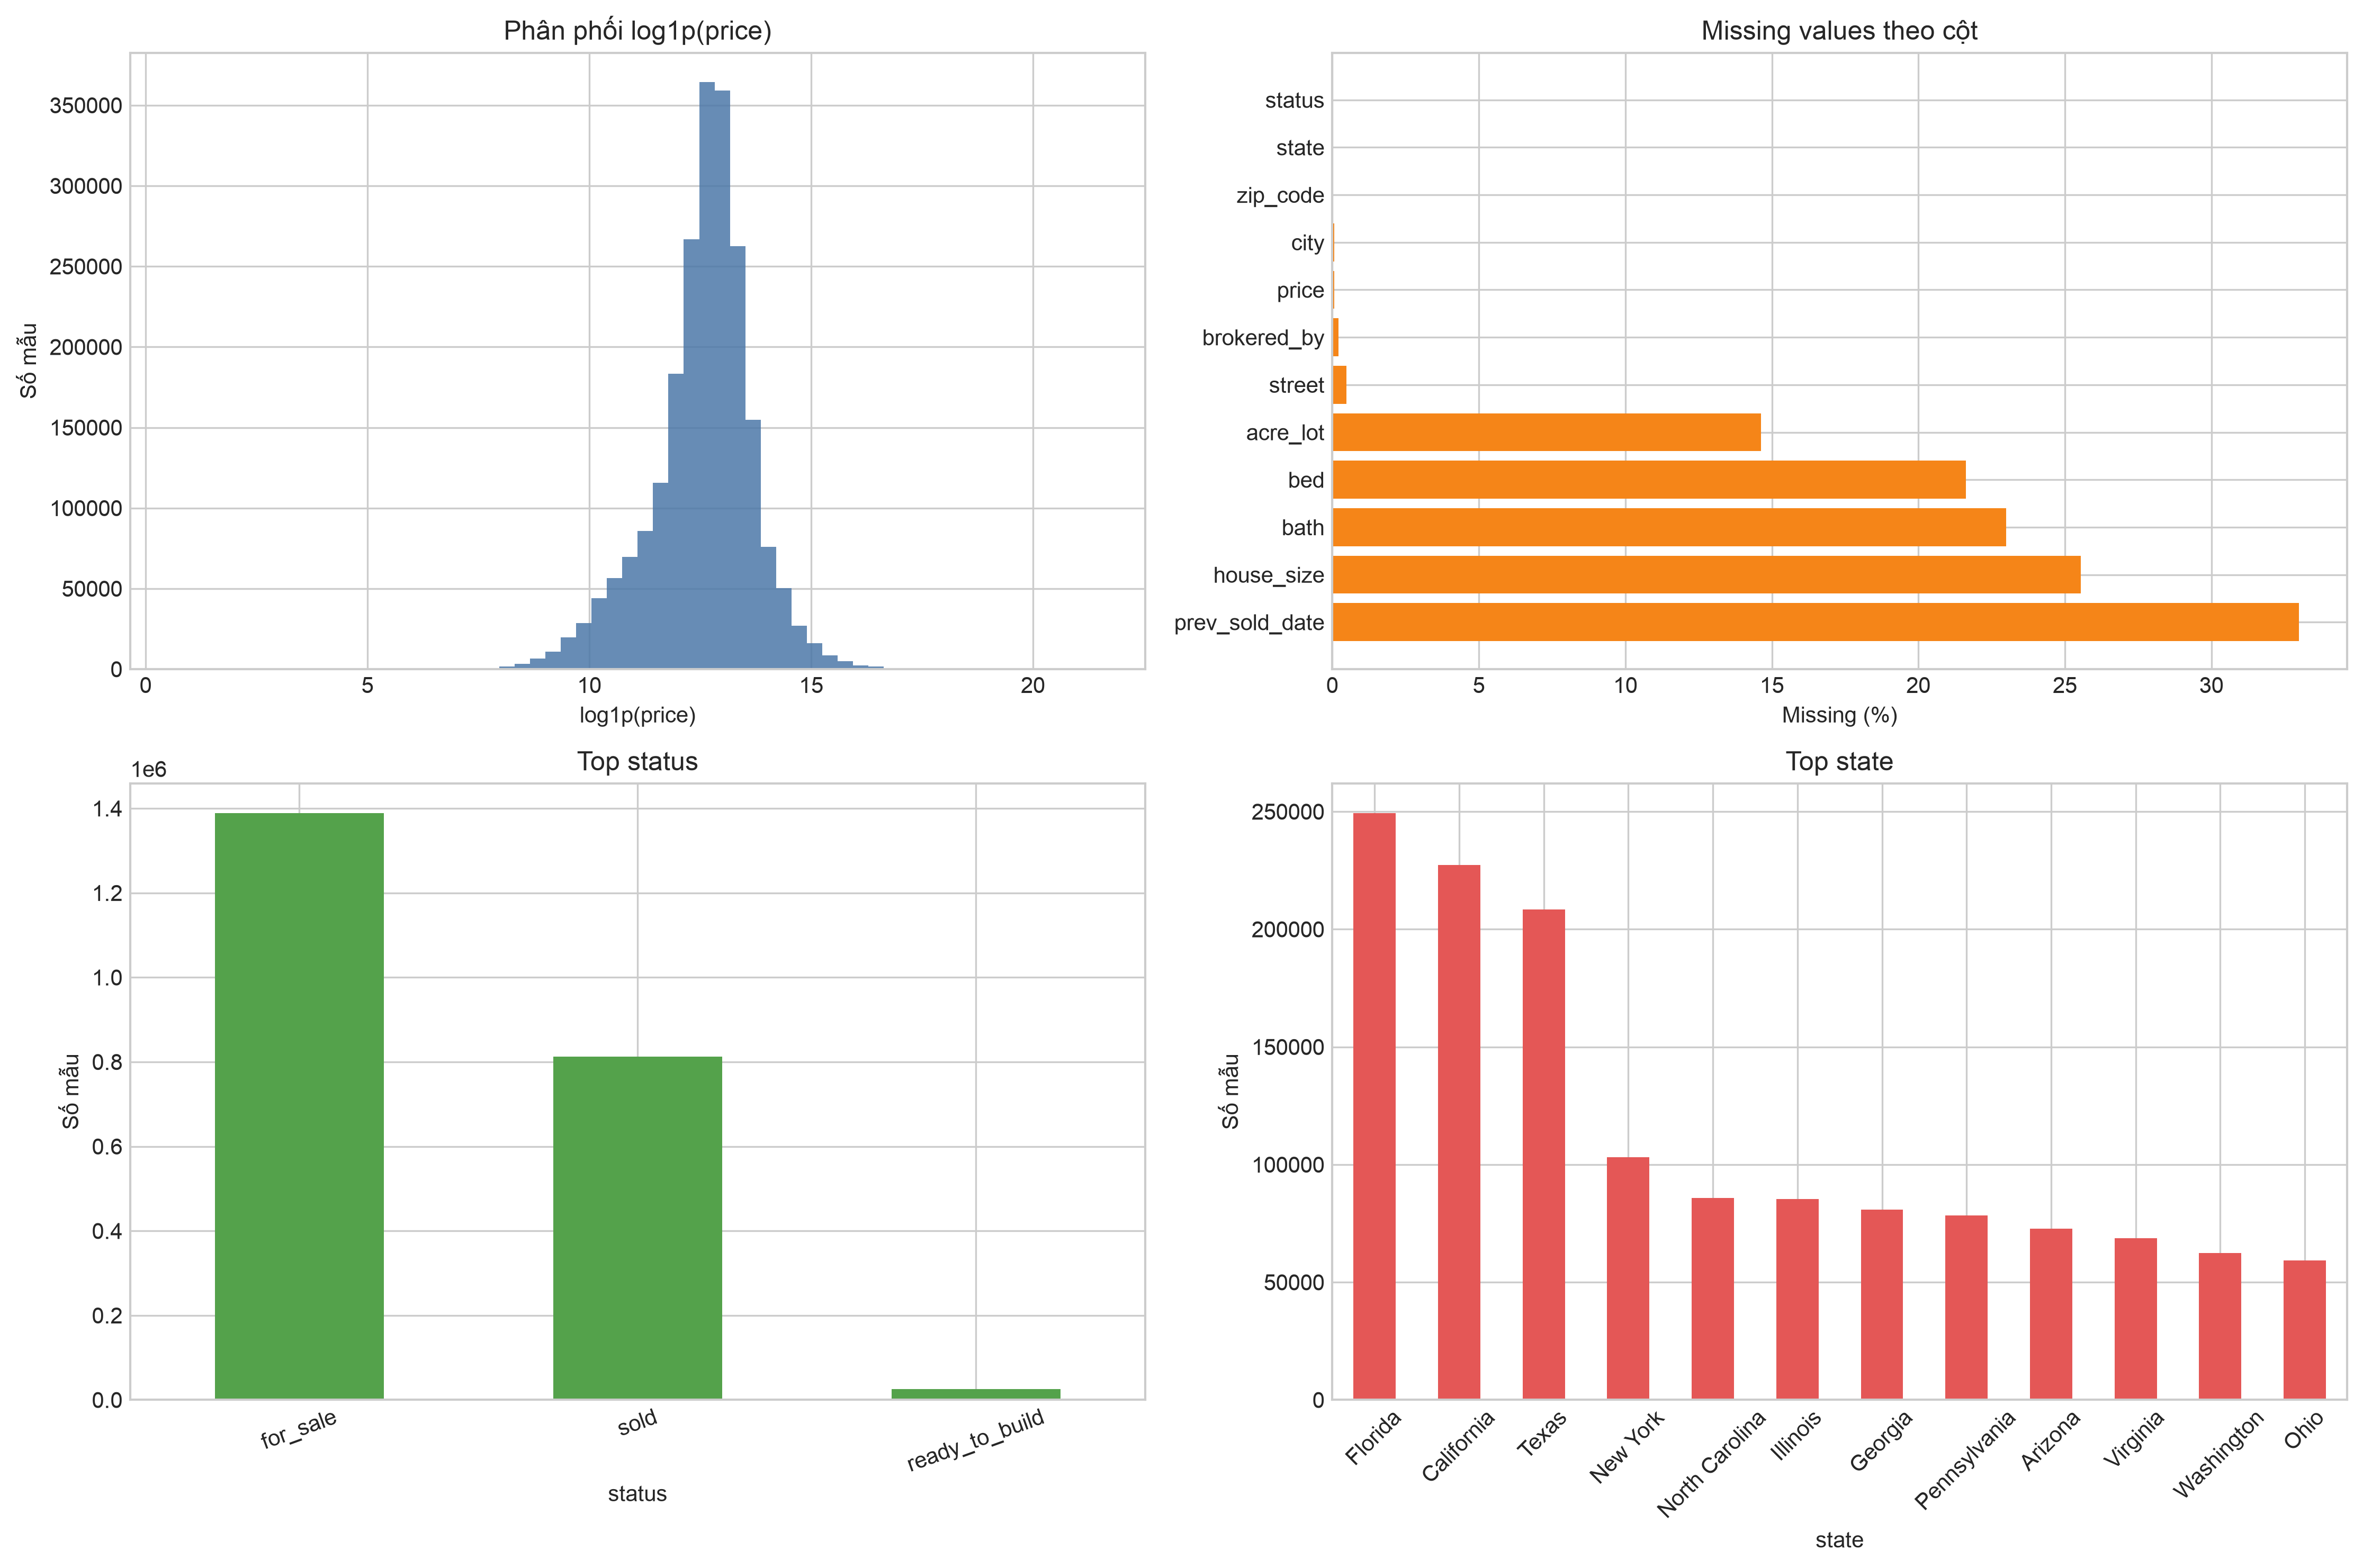
\includegraphics[width=\textwidth]{house_price_eda_overview.png}
    \caption{Tổng quan EDA: phân phối log-price, missing values, status và state}
    \label{fig:house_price_eda}
\end{figure}

\begin{figure}[H]
    \centering
    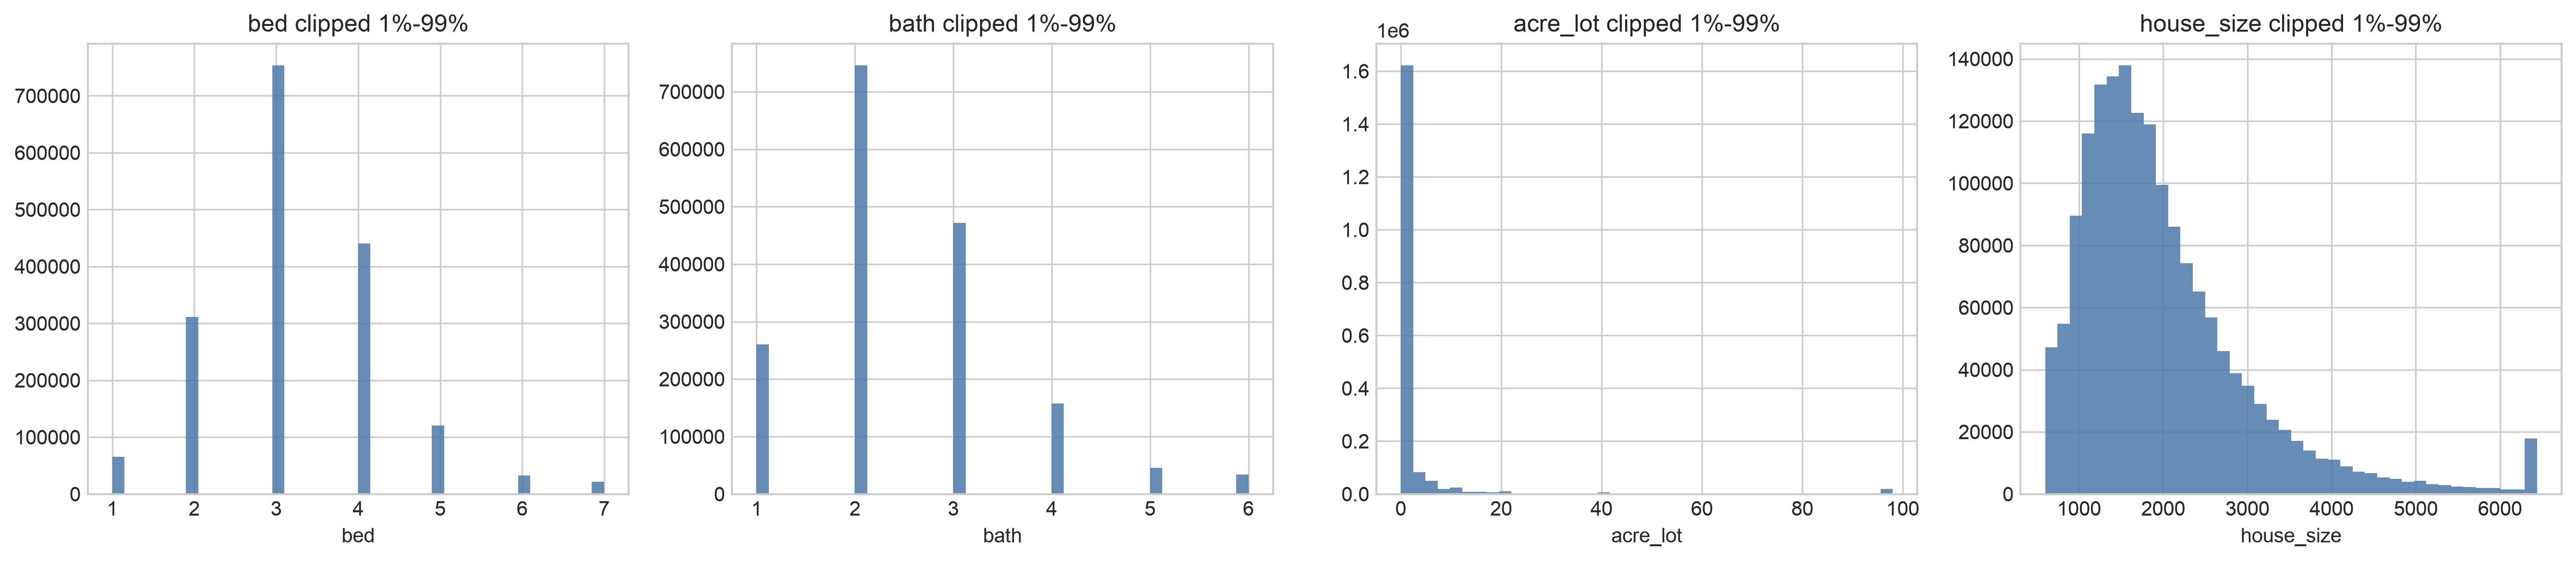
\includegraphics[width=\textwidth]{house_price_numeric_feature_distributions.png}
    \caption{Phân phối các đặc trưng số chính sau clipping 1\%--99\%}
    \label{fig:house_price_numeric}
\end{figure}

\section{Bốn cấu hình hồi quy}
Notebook huấn luyện Ridge Regression, Decision Tree Regressor, Random Forest Regressor và MLP thuần NumPy kiến trúc $input \to 128 \to 64 \to 32 \to 1$. MLP dùng ReLU, output tuyến tính, Adam optimizer viết bằng NumPy, L2 regularization và early stopping theo validation RMSLE.

\subsection{Vai trò của từng baseline hồi quy}
Ridge Regression đại diện cho baseline tuyến tính có regularization.
Nếu Ridge đạt kết quả tốt, điều đó cho thấy feature engineering đã tuyến tính hóa phần lớn quan hệ giữa dữ liệu và log-price.
Decision Tree Regressor kiểm tra khả năng mô hình hóa quy tắc phi tuyến dạng phân vùng.
Random Forest giảm phương sai của tree đơn bằng cách trung bình hóa nhiều cây, nhưng chi phí dự đoán và khả năng giải thích chi tiết thường cao hơn.

MLP NumPy được kỳ vọng tận dụng tốt các quan hệ phi tuyến mềm giữa diện tích, vị trí, trạng thái và thời gian.
Khác với tree, MLP học biểu diễn liên tục.
Điều này có lợi khi quan hệ giá không phải là các ngưỡng rời rạc hoàn toàn mà thay đổi mượt theo nhiều đặc trưng.

\begin{figure}[H]
    \centering
    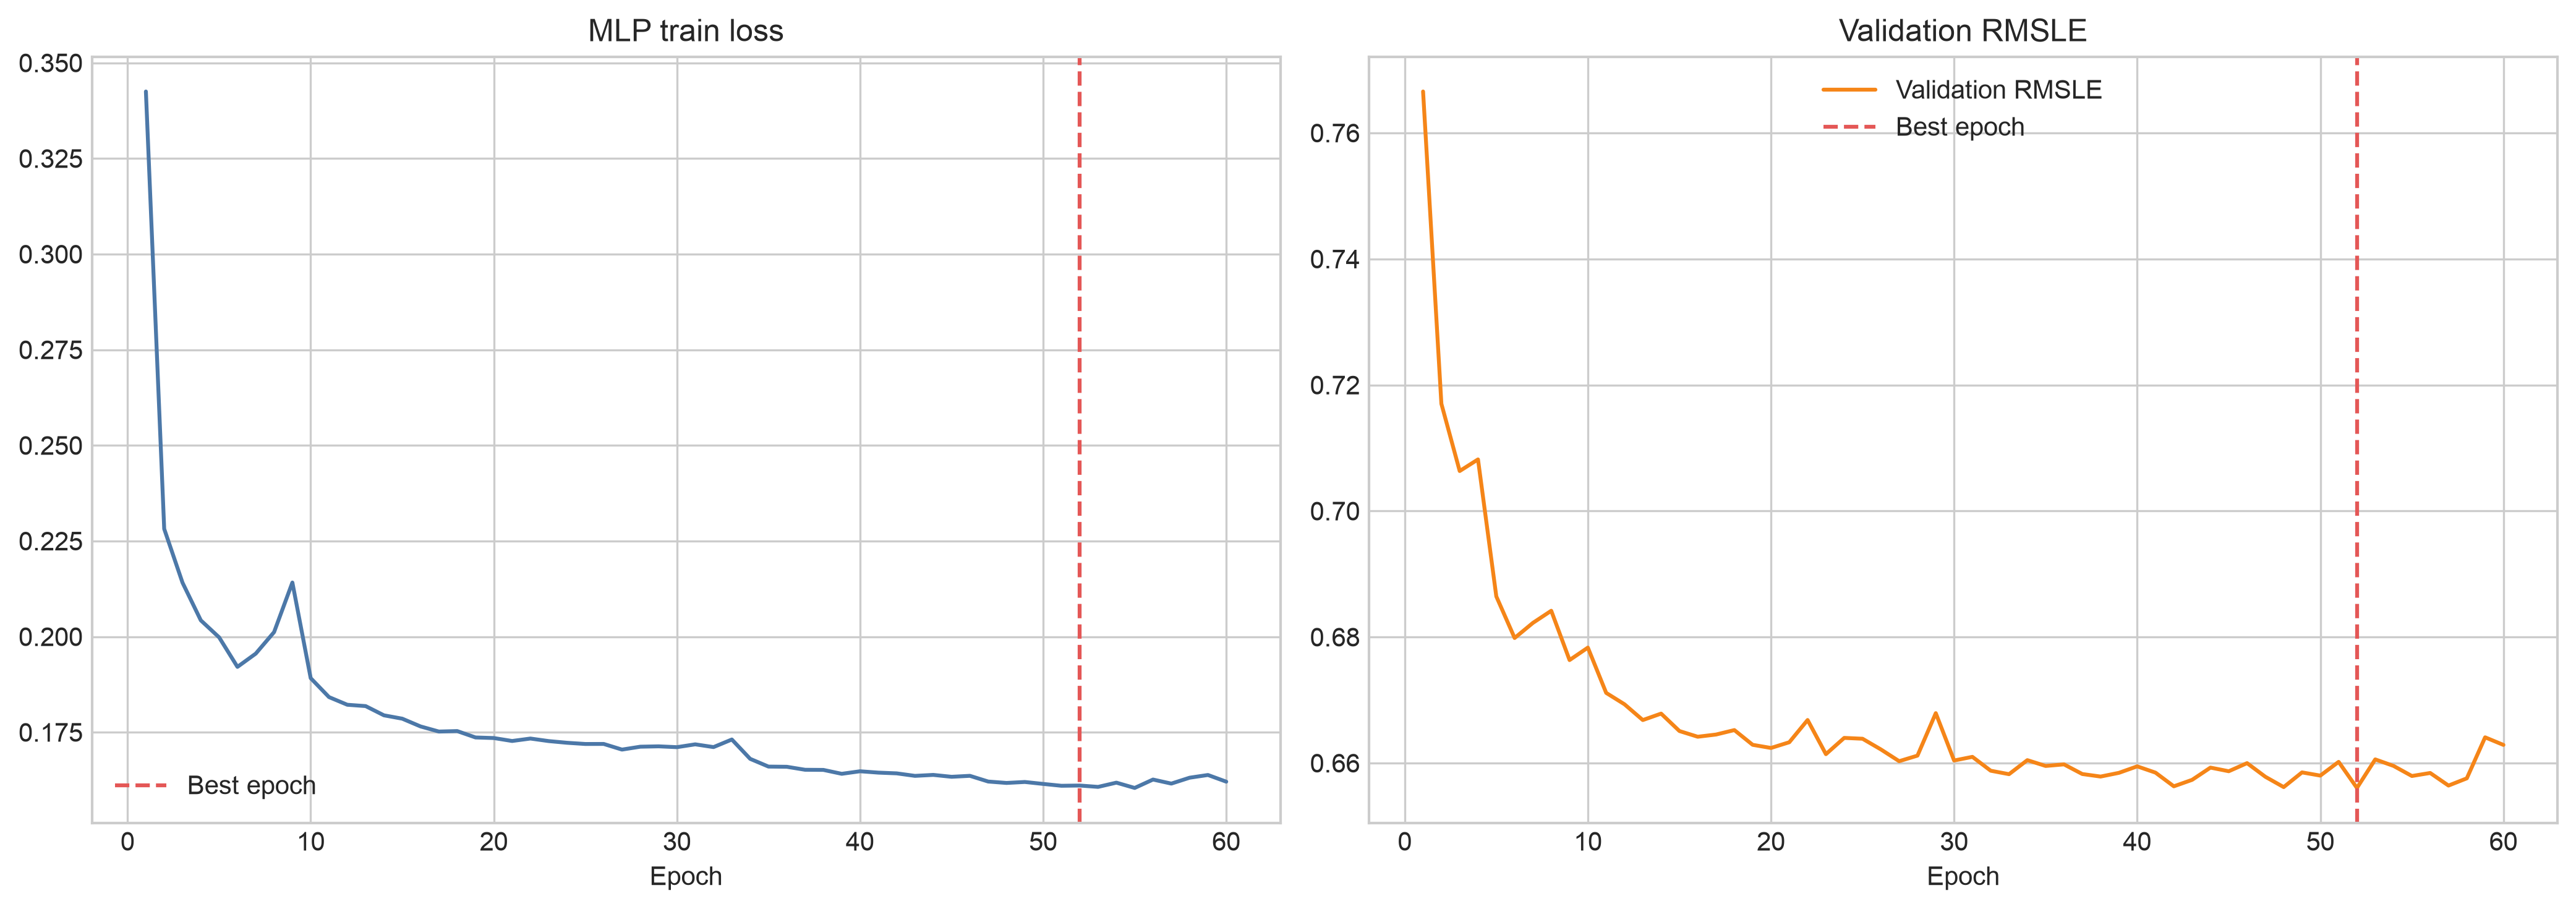
\includegraphics[width=0.95\textwidth]{house_price_mlp_learning_curve.png}
    \caption{Learning curve của MLP NumPy trên bài toán định giá nhà}
    \label{fig:house_price_learning_curve}
\end{figure}

\section{Kết quả và phân tích sai số}
MLP NumPy đạt kết quả tốt nhất theo RMSLE, MAE và $R^2$. Điều này cho thấy biến đổi log-price kết hợp mạng phi tuyến học được quan hệ phức tạp hơn giữa đặc trưng vị trí, diện tích và giá nhà.

\subsection{Diễn giải sai số}
MAE khoảng \$217,538 của MLP nghĩa là trung bình dự đoán lệch khoảng 217 nghìn USD trên test set.
Con số này lớn, nhưng cần đặt trong bối cảnh dataset bất động sản toàn nước Mỹ có biên giá rất rộng.
MedianAE 77,432 thấp hơn nhiều so với MAE, cho thấy phần lớn dự đoán có sai số vừa phải hơn, còn MAE bị kéo lên bởi các outlier.

RMSE hơn 1 triệu USD xác nhận rằng vẫn tồn tại những trường hợp sai số rất lớn.
Đây là lý do residual analysis trong Hình \ref{fig:house_price_residual} quan trọng.
Trong notebook, biểu đồ này được tạo từ tối đa 5,000 mẫu test và residual được tính bằng \texttt{actual - predicted}.

\begin{table}[H]
\centering
\caption{Benchmark 4 mô hình hồi quy trên house price}
\label{tab:house_price_benchmark}
\resizebox{\textwidth}{!}{%
\begin{tabular}{lrrrrrrr}
\toprule
\textbf{Mô hình} & \textbf{MAE} & \textbf{RMSE} & \textbf{MedianAE} & \textbf{MAPE} & \textbf{RMSLE} & \textbf{$R^2$} & \textbf{Train(s)} \\
\midrule
NumPy MLP (128-64-32) & \textbf{217,538} & \textbf{1,094,000} & \textbf{77,432} & 34.6065 & \textbf{0.6578} & \textbf{0.3354} & 16.7879 \\
Decision Tree Regressor & 241,108 & 1,169,300 & 87,561 & 49.5228 & 0.7205 & 0.2408 & 0.9791 \\
Random Forest Regressor & 247,668 & 1,241,500 & 87,537 & \textbf{26.1412} & 0.7216 & 0.1442 & 0.8762 \\
Ridge Regression & 268,912 & 1,228,200 & 92,871 & 28.7193 & 0.7717 & 0.1624 & \textbf{0.3712} \\
\bottomrule
\end{tabular}%
}
\end{table}

\begin{figure}[H]
    \centering
    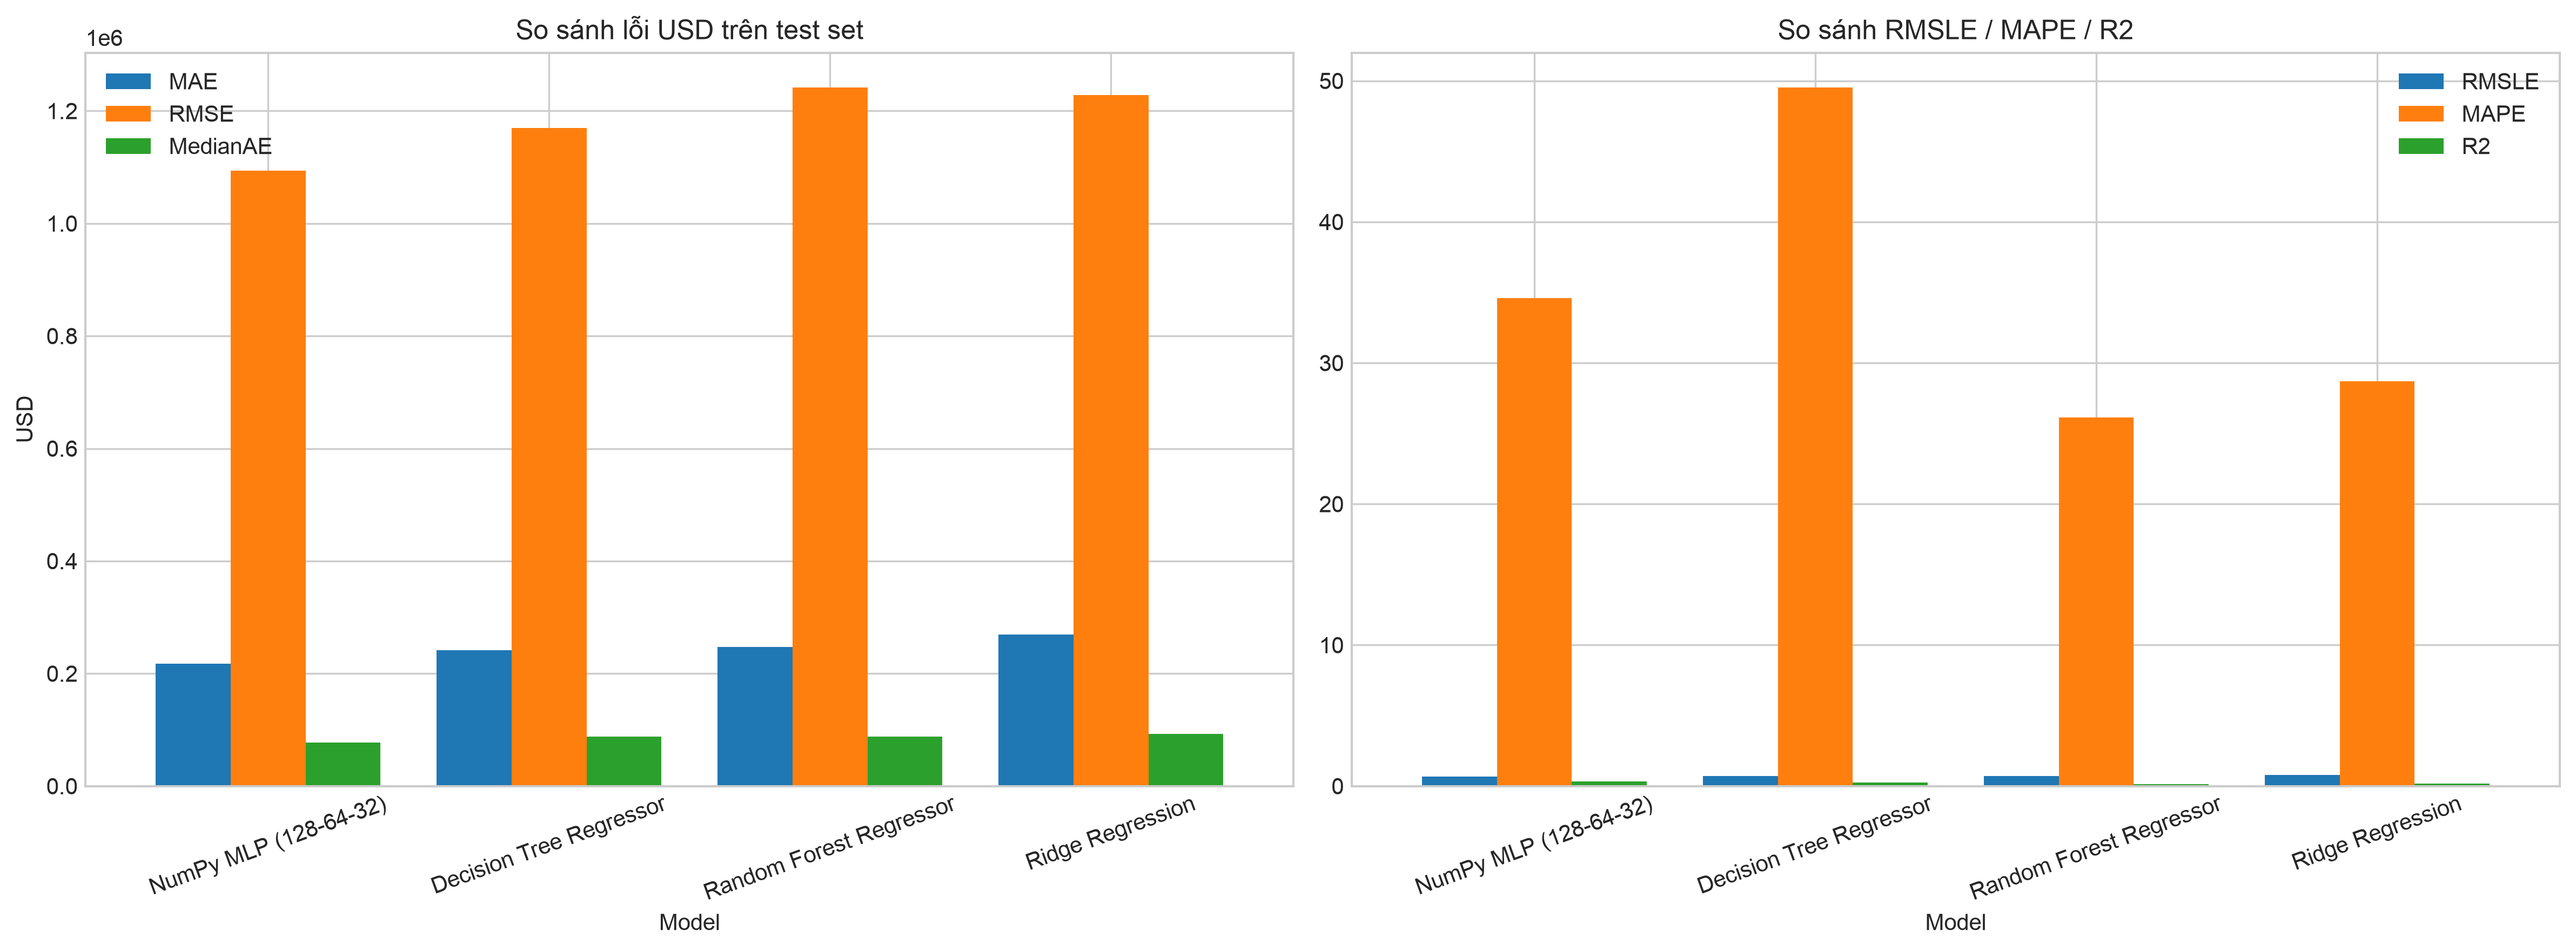
\includegraphics[width=\textwidth]{house_price_metric_comparison.png}
    \caption{So sánh metric hồi quy trên house price}
    \label{fig:house_price_metric_comparison}
\end{figure}

\begin{figure}[H]
    \centering
    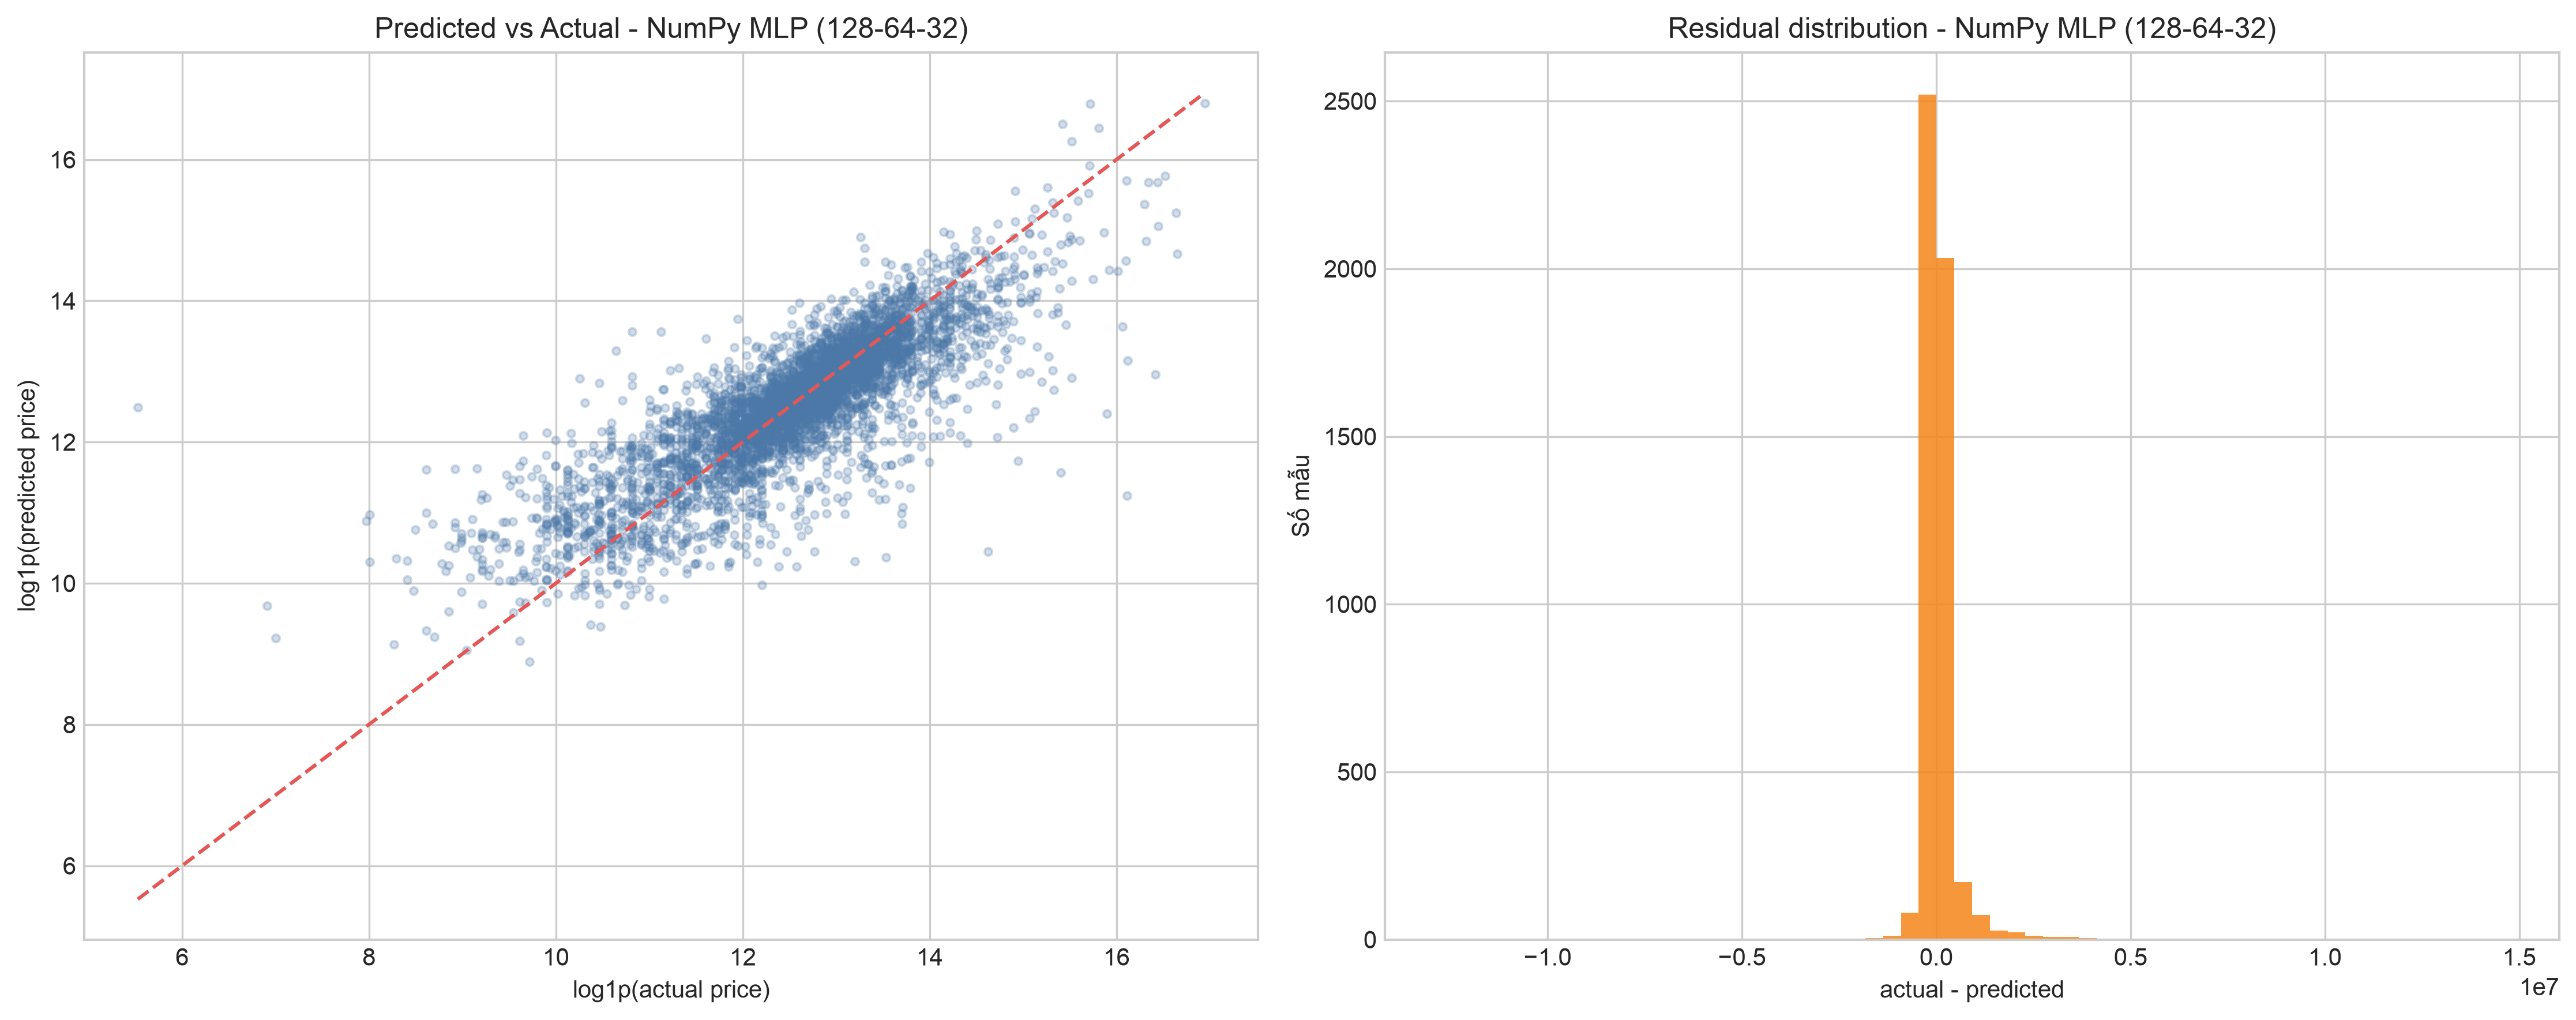
\includegraphics[width=\textwidth]{house_price_residual_analysis.png}
    \caption{Residual analysis của mô hình tốt nhất}
    \label{fig:house_price_residual}
\end{figure}

\begin{figure}[H]
    \centering
    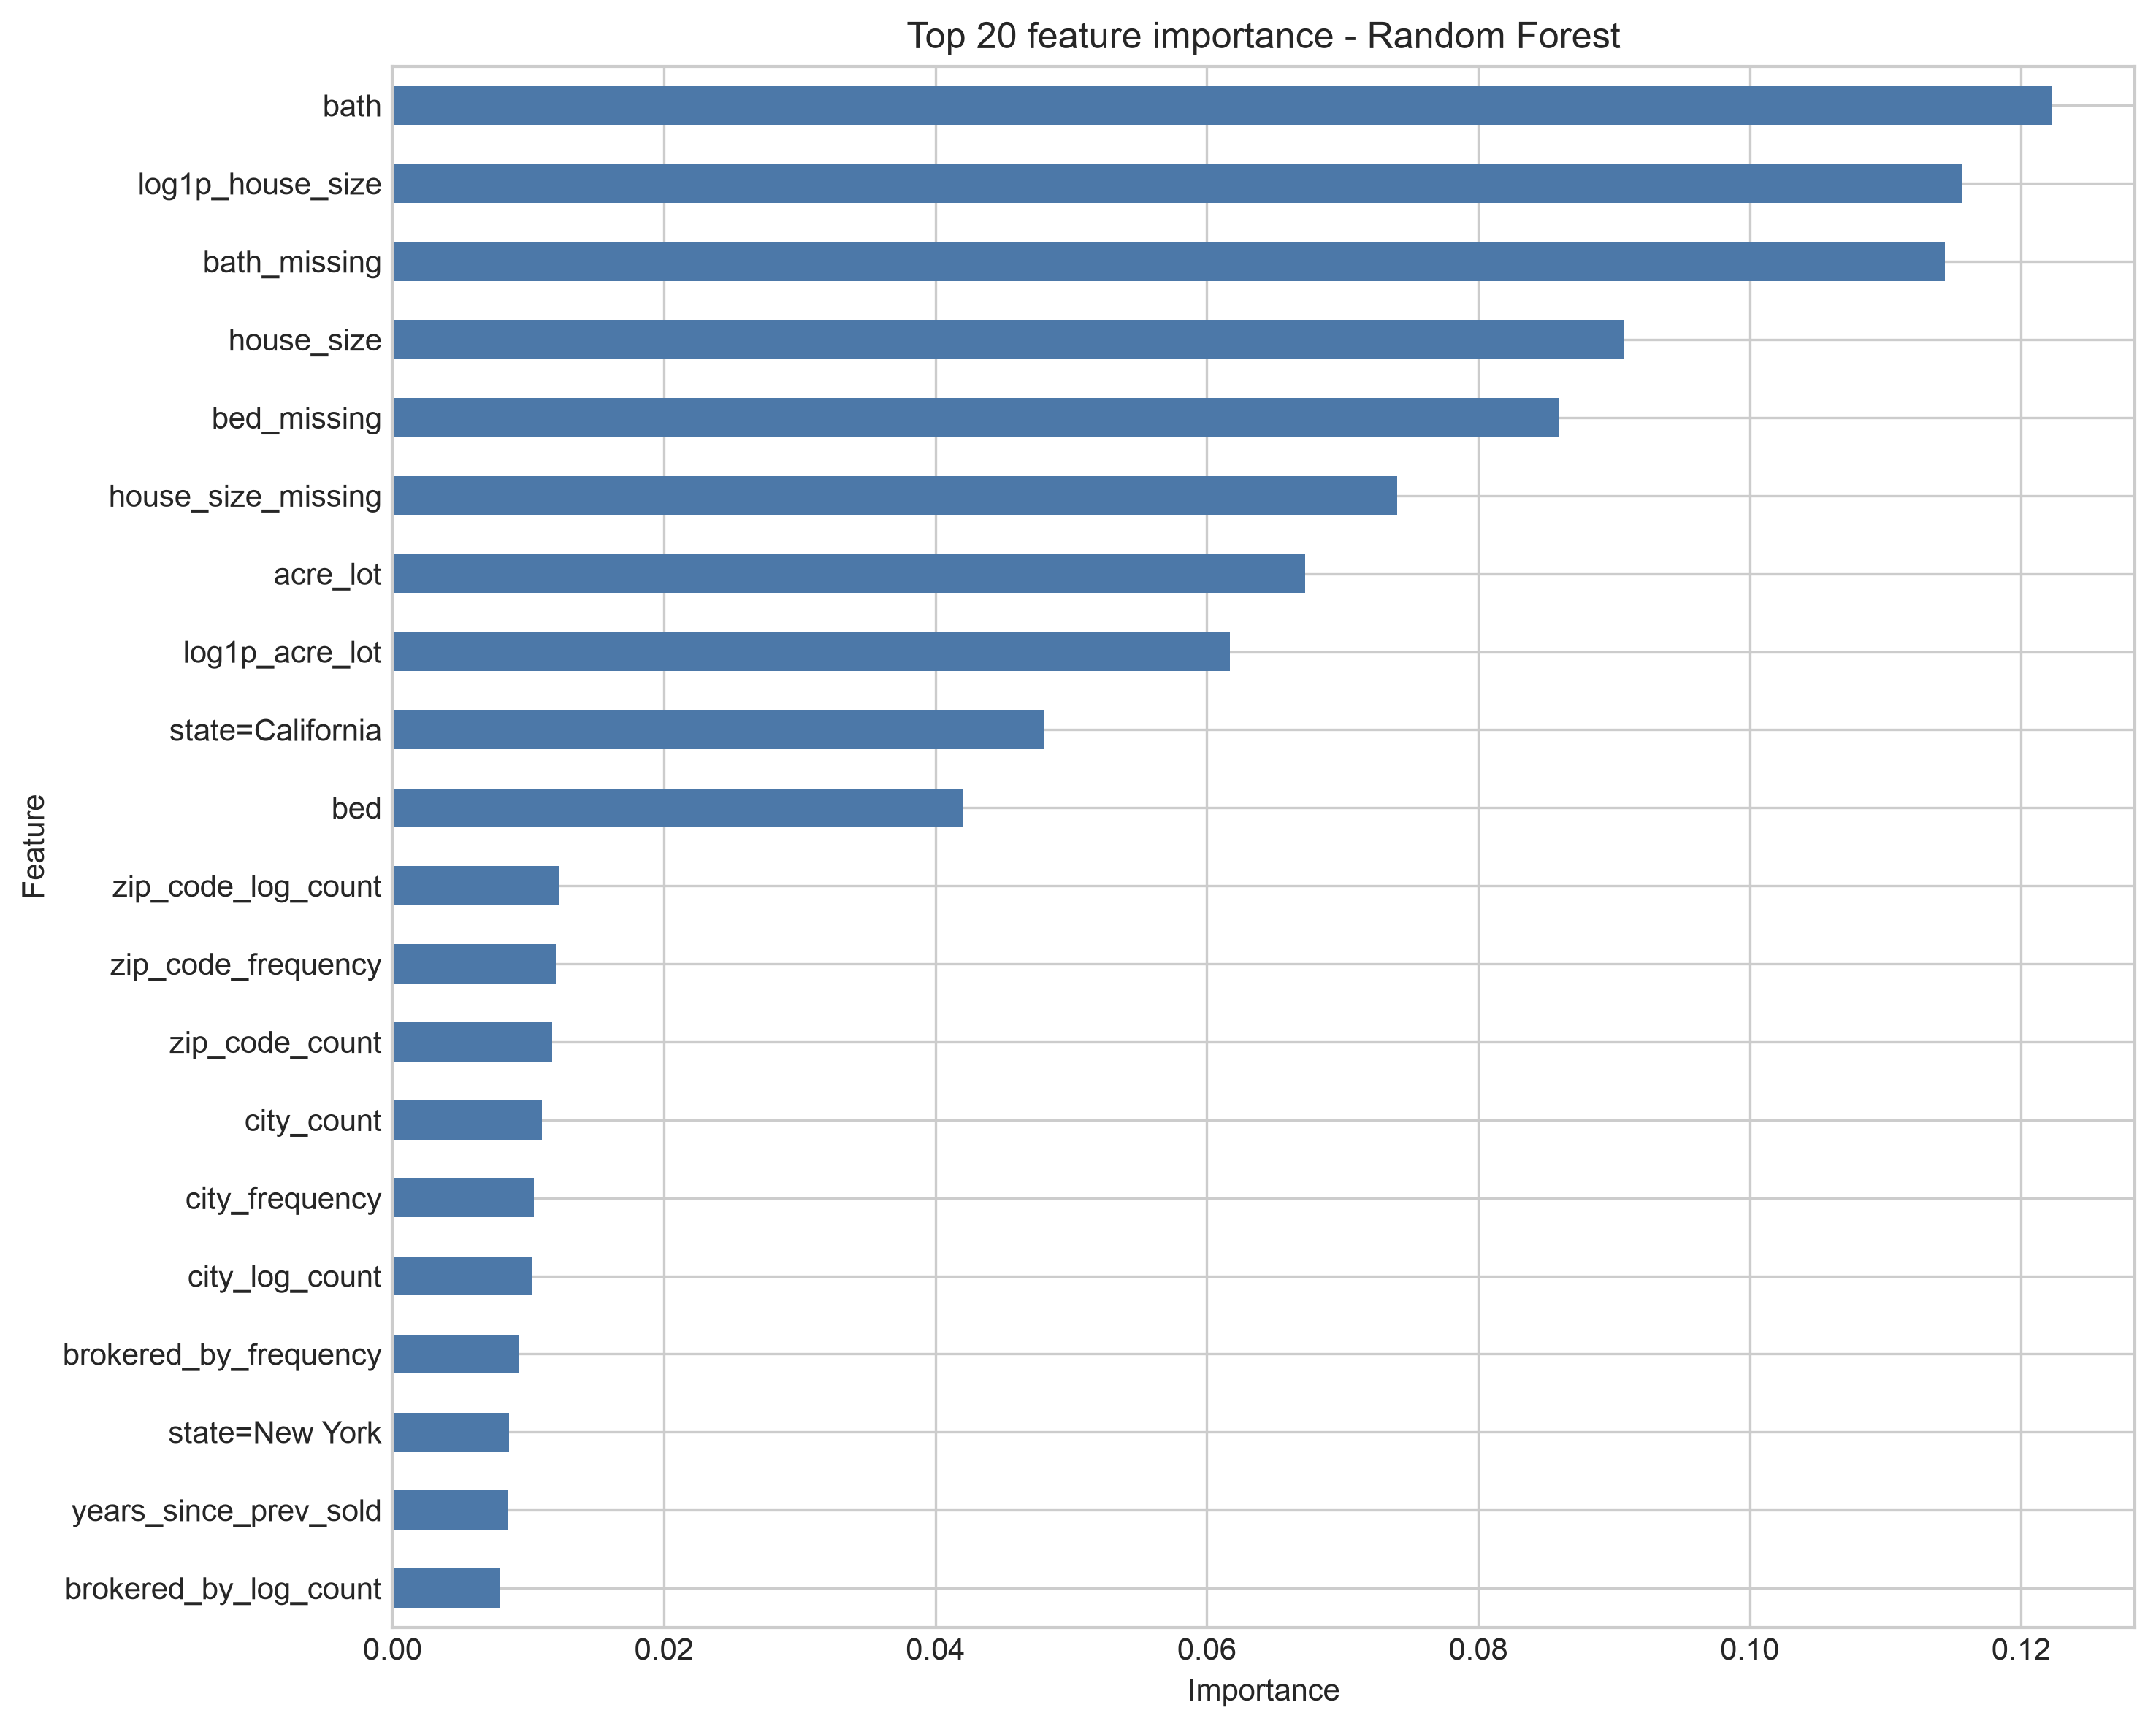
\includegraphics[width=0.95\textwidth]{house_price_random_forest_feature_importance.png}
    \caption{Top feature importance của Random Forest}
    \label{fig:house_price_feature_importance}
\end{figure}

% =========================================================================
% CHUONG 5
% =========================================================================
\chapter{Customer Comments: Phân Loại Trên TF--IDF}

\section{Dữ liệu văn bản và nhãn dự đoán}
Notebook \modelpath{Assignment3/customer\_comments/notebook/customer\_comments\_benchmark.ipynb} sử dụng dataset \modelpath{Womens Clothing E-Commerce Reviews.csv}. Mục tiêu là dự đoán nhãn \texttt{Recommended IND} từ nội dung \texttt{Title + Review Text}. Sau khi bỏ review rỗng, còn 22,642 mẫu; tỷ lệ recommend chiếm đa số nên notebook đánh giá bằng nhiều chỉ số.

\subsection{Đặc thù phân loại review}
Bài toán review khác với dữ liệu bảng vì tín hiệu nằm trong ngôn ngữ tự nhiên.
Một vài từ như ``perfect'', ``love'', ``return'', ``small'' hoặc ``disappointed'' có thể tác động mạnh đến nhãn khuyến nghị.
Tuy nhiên văn bản cũng chứa nhiễu: viết tắt, lỗi chính tả, câu rất ngắn, câu rất dài và thông tin không liên quan.
Do đó bước làm sạch văn bản ảnh hưởng trực tiếp đến chất lượng vector TF-IDF.

\section{Từ văn bản thô đến 1,000 đặc trưng TF--IDF}
Văn bản được chuyển lowercase, loại HTML/URL/ký tự không phải chữ, chuẩn hóa khoảng trắng. Dữ liệu được chia train/test 80/20 theo stratified split. \texttt{TfidfVectorizer} tạo đúng 1,000 đặc trưng và chỉ \texttt{fit\_transform} trên train, test chỉ \texttt{transform} để chống rò rỉ dữ liệu.

\subsection{TF-IDF 1,000 chiều fit nghiêm ngặt trên train}
Yêu cầu quan trọng của notebook là vocabulary 1,000 từ phải được học từ train set.
Nếu vectorizer nhìn thấy toàn bộ dữ liệu trước khi split, những từ chỉ xuất hiện trong test set có thể lọt vào vocabulary.
Khi đó mô hình không trực tiếp nhìn nhãn test, nhưng vẫn được hưởng thông tin phân phối từ test, tạo leakage tinh vi.

Với TF-IDF, mỗi feature phản ánh đồng thời tần suất trong một review và độ hiếm trên toàn bộ train corpus.
Các từ phổ biến ở mọi review bị giảm trọng số, còn các từ mang sắc thái cảm xúc hoặc đặc trưng sản phẩm thường nổi bật hơn.
Giới hạn 1,000 chiều giữ cho MLP NumPy chạy nhanh, đồng thời vẫn đủ rộng để Logistic Regression và Naive Bayes phát huy thế mạnh trên dữ liệu thưa.

\begin{figure}[H]
    \centering
    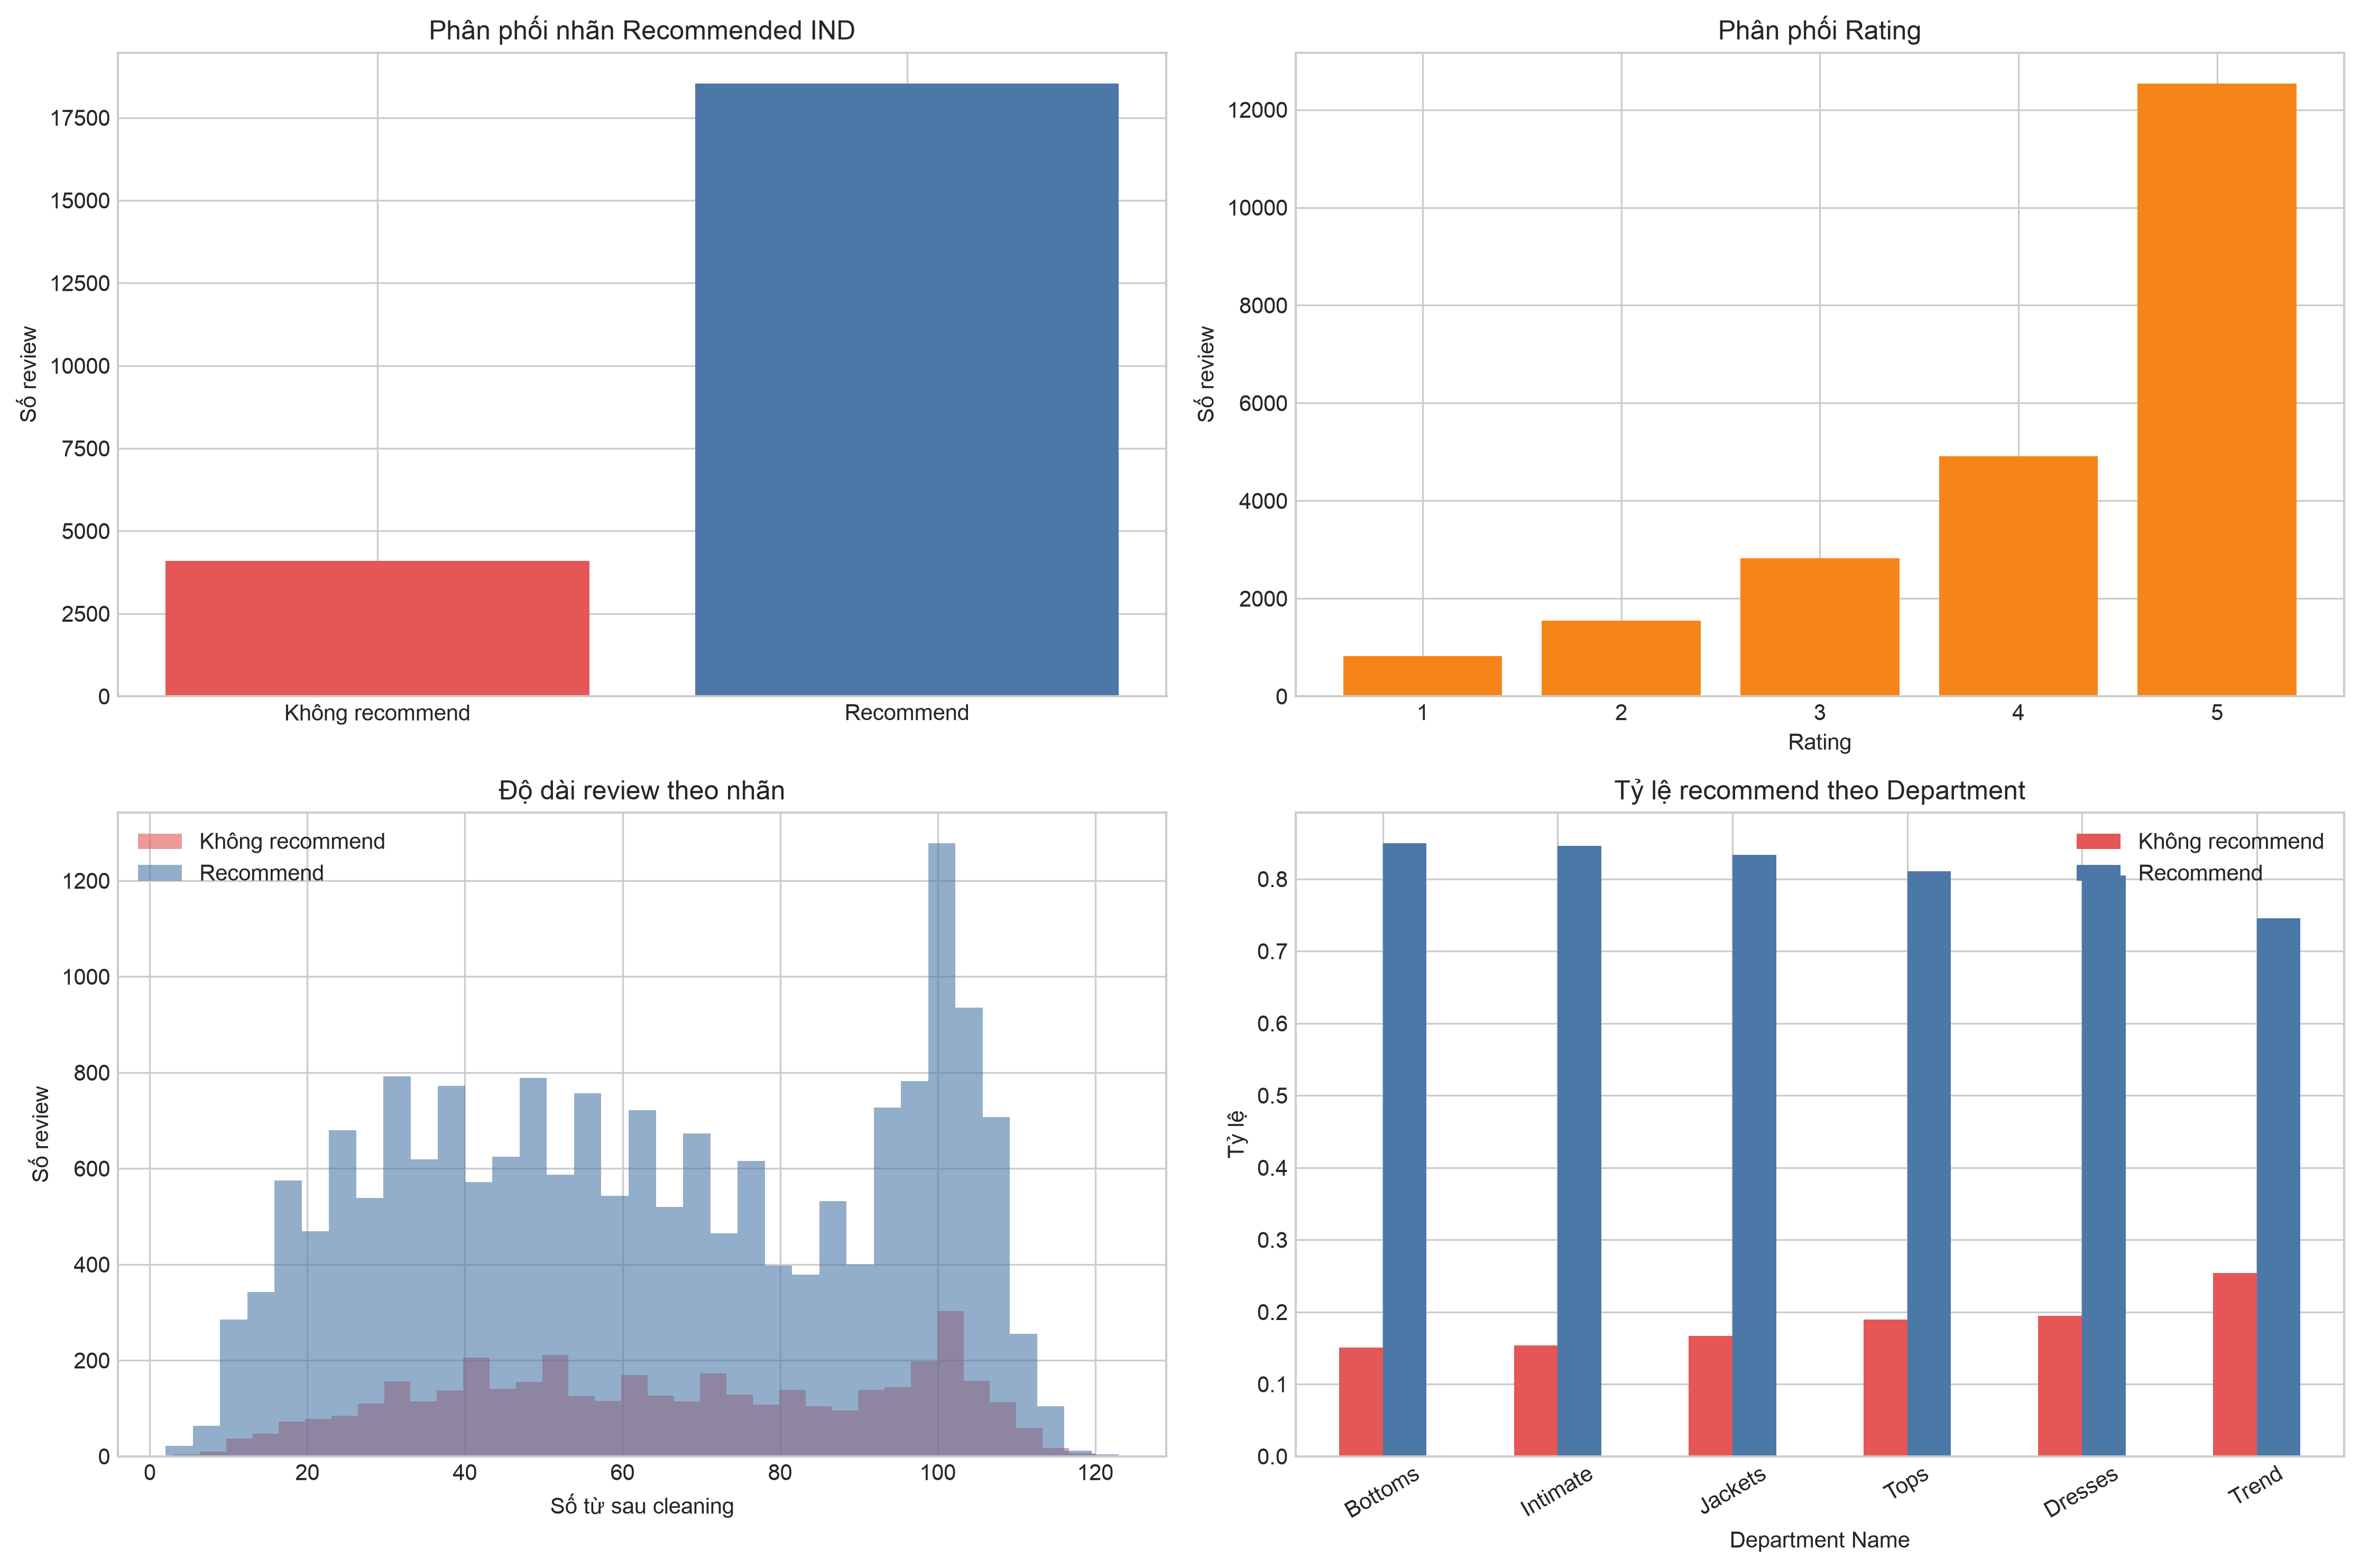
\includegraphics[width=\textwidth]{customer_comments_eda_overview.png}
    \caption{EDA dữ liệu review: phân phối nhãn, rating, độ dài review và tỷ lệ recommend theo department}
    \label{fig:comments_eda}
\end{figure}

\begin{figure}[H]
    \centering
    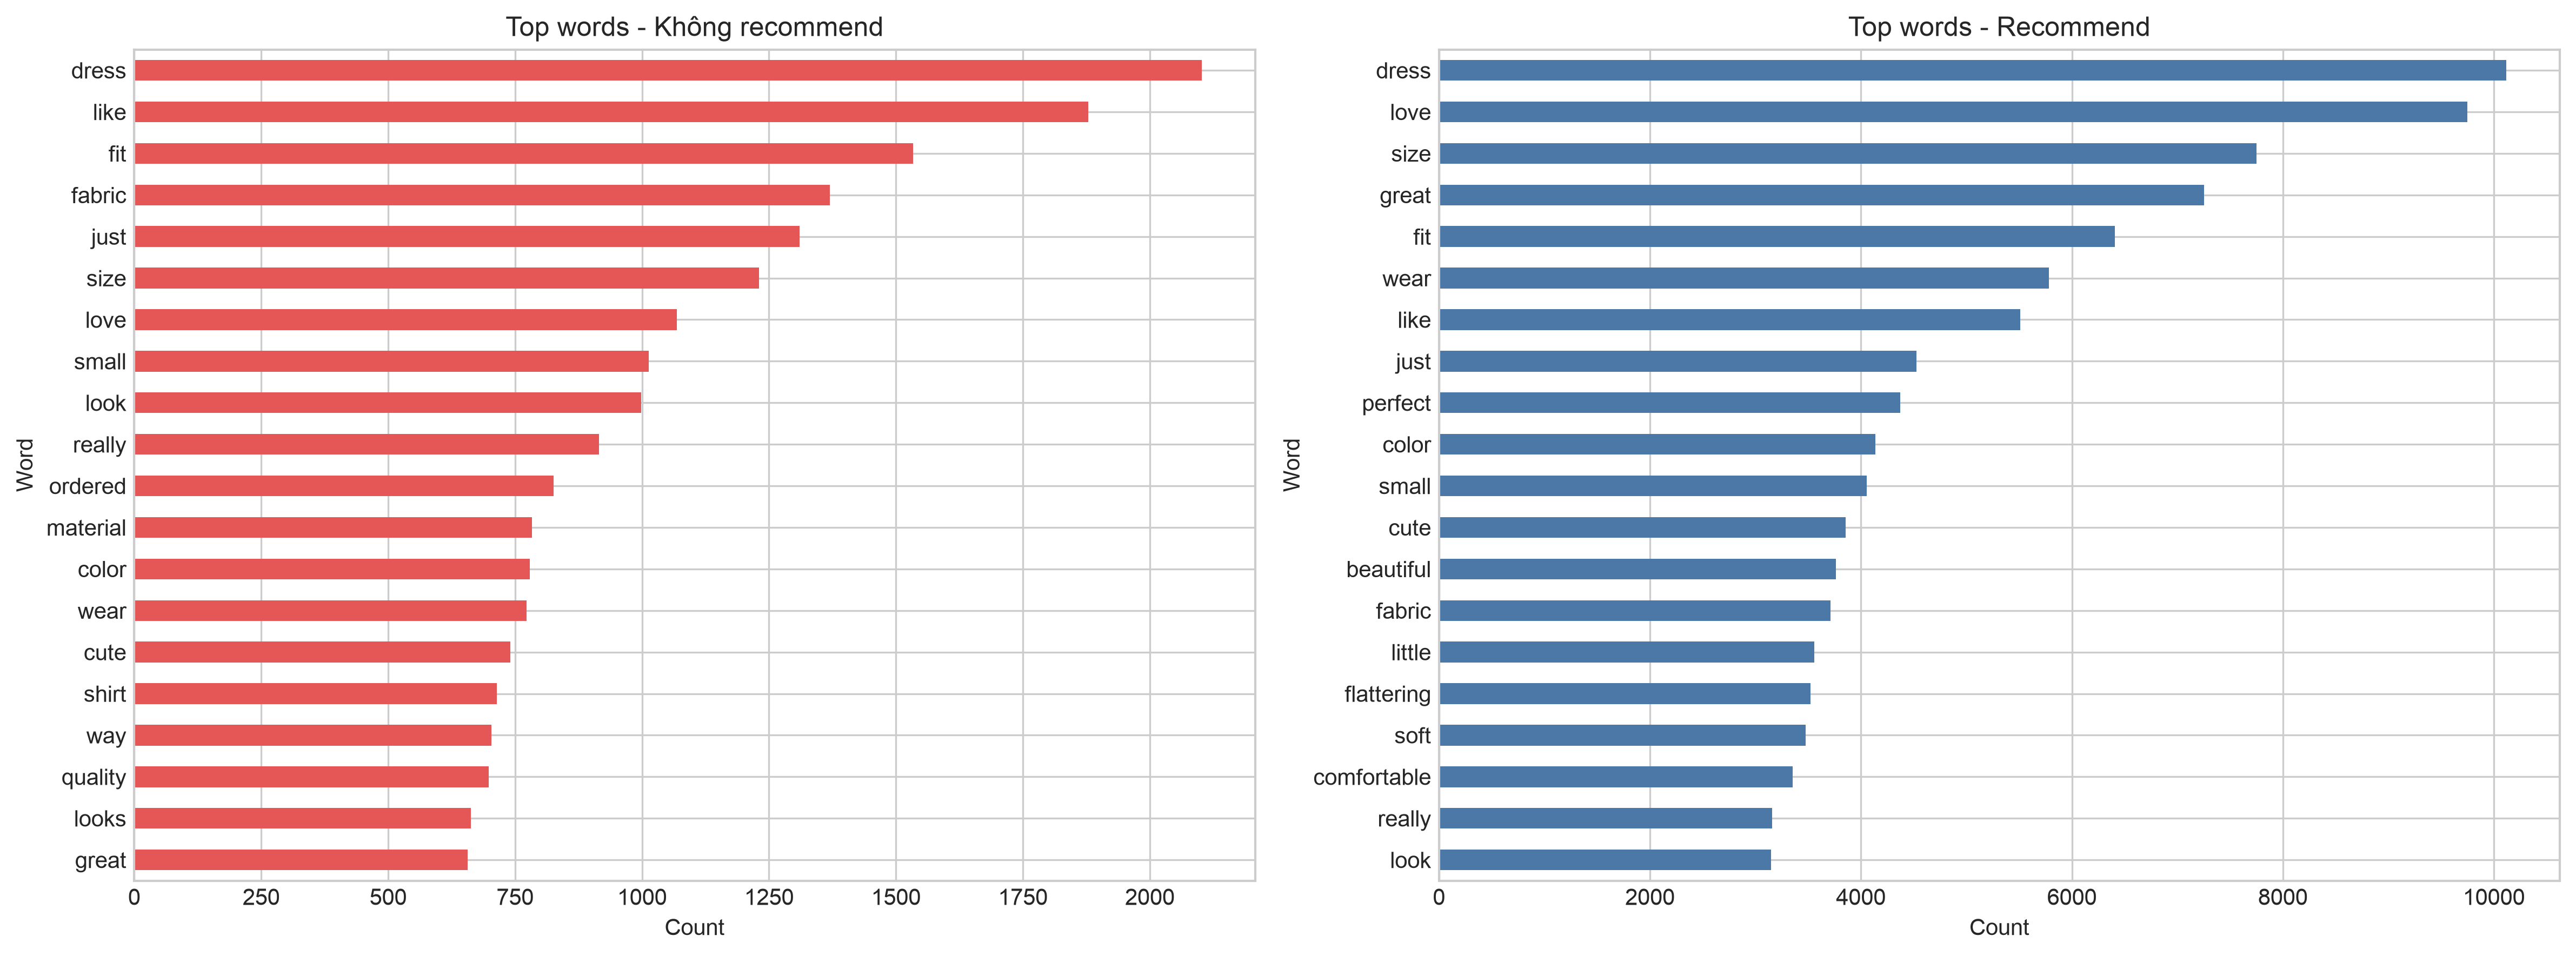
\includegraphics[width=\textwidth]{customer_comments_top_words_by_label.png}
    \caption{Top words theo từng nhãn sau làm sạch văn bản}
    \label{fig:comments_top_words}
\end{figure}

\begin{figure}[H]
    \centering
    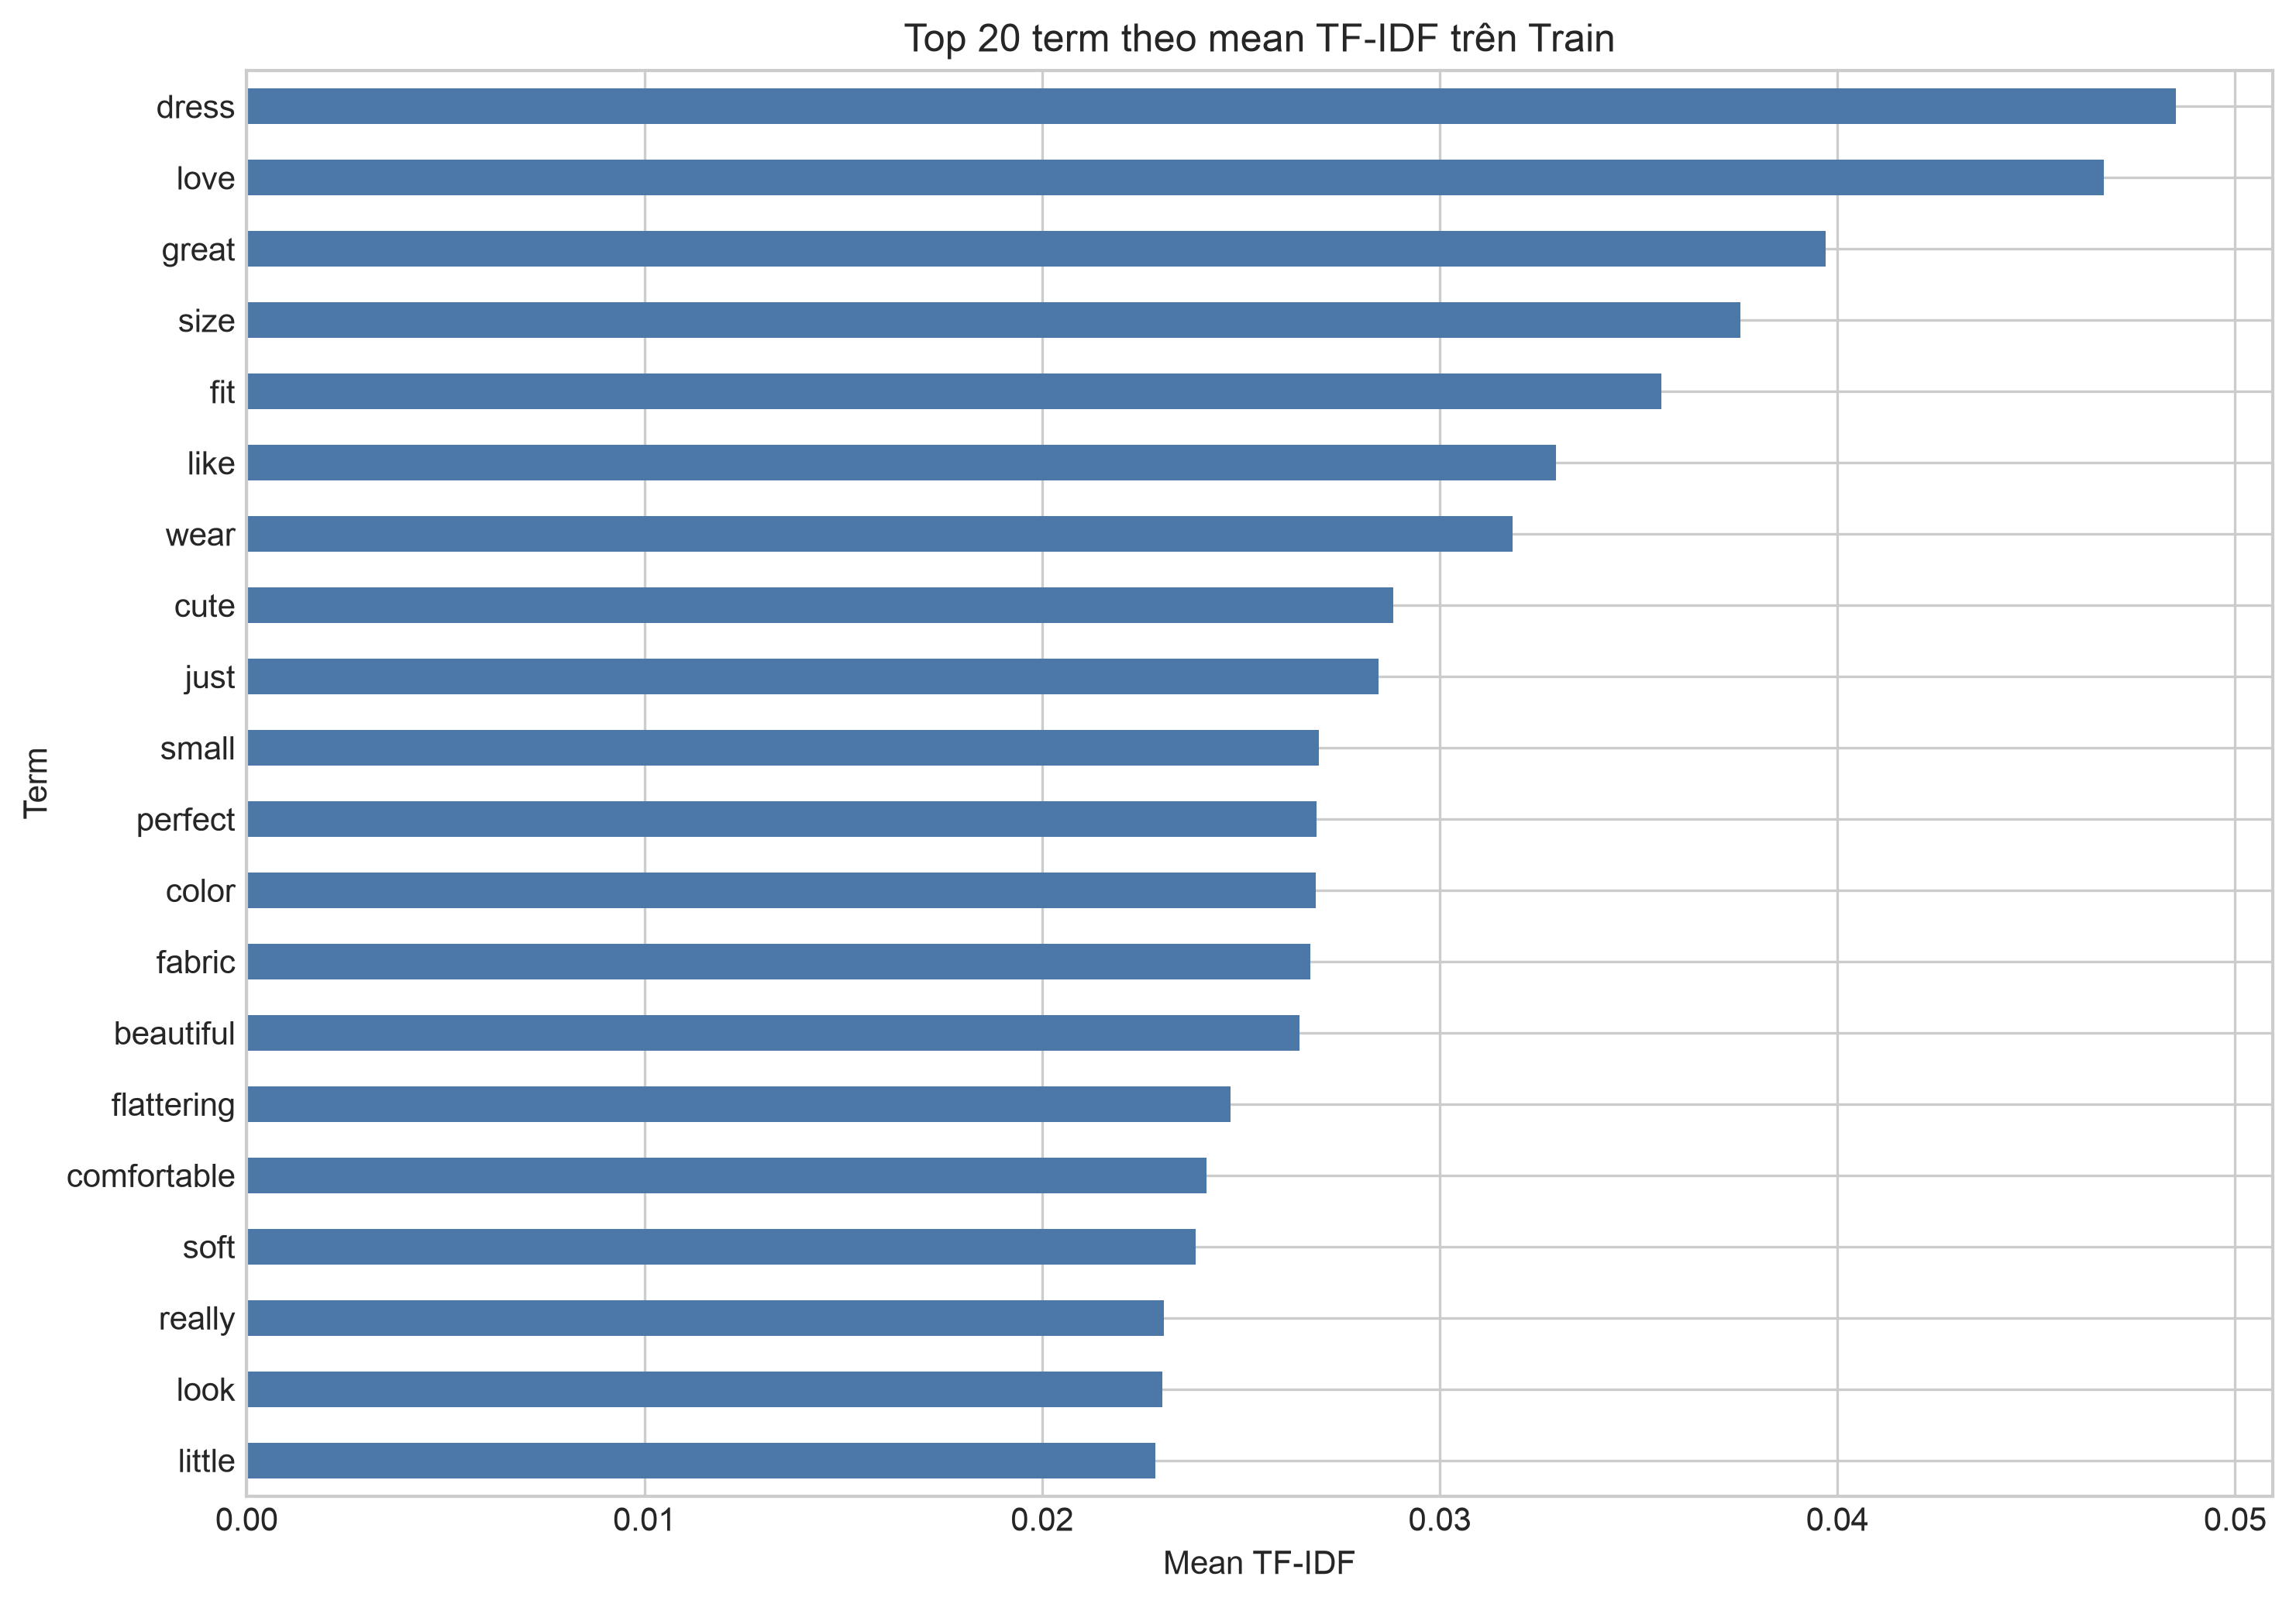
\includegraphics[width=0.95\textwidth]{customer_comments_top_tfidf_terms.png}
    \caption{Top terms theo mean TF-IDF trên tập train}
    \label{fig:comments_tfidf}
\end{figure}

\section{Các mô hình phân loại}
Bốn mô hình được huấn luyện gồm Logistic Regression, Multinomial Naive Bayes, Random Forest và MLP thuần NumPy kiến trúc $1000 \to 64 \to 16 \to 1$. MLP dùng ReLU, sigmoid, Binary Cross-Entropy có class weighting và Mini-batch Gradient Descent.

\subsection{Vì sao Naive Bayes mạnh trên TF-IDF}
Multinomial Naive Bayes thường là baseline rất mạnh cho phân loại văn bản.
Mô hình giả định đóng góp của từng từ gần độc lập, một giả định đơn giản nhưng thường đủ tốt khi feature là bag-of-words hoặc TF-IDF.
Kết quả F1 0.9212 cho thấy review có nhiều tín hiệu từ vựng trực tiếp về việc khách hàng có khuyến nghị sản phẩm hay không.

Logistic Regression đạt ROC-AUC cao nhất 0.9348.
Điều này cho thấy mô hình tuyến tính xếp hạng xác suất tốt trên nhiều ngưỡng.
MLP NumPy đạt F1 0.9091 và ROC-AUC 0.9297, khá sát các baseline mạnh.
Random Forest kém hơn một chút vì tree-based model thường không tận dụng tốt không gian sparse high-dimensional bằng mô hình tuyến tính hoặc xác suất.

\begin{figure}[H]
    \centering
    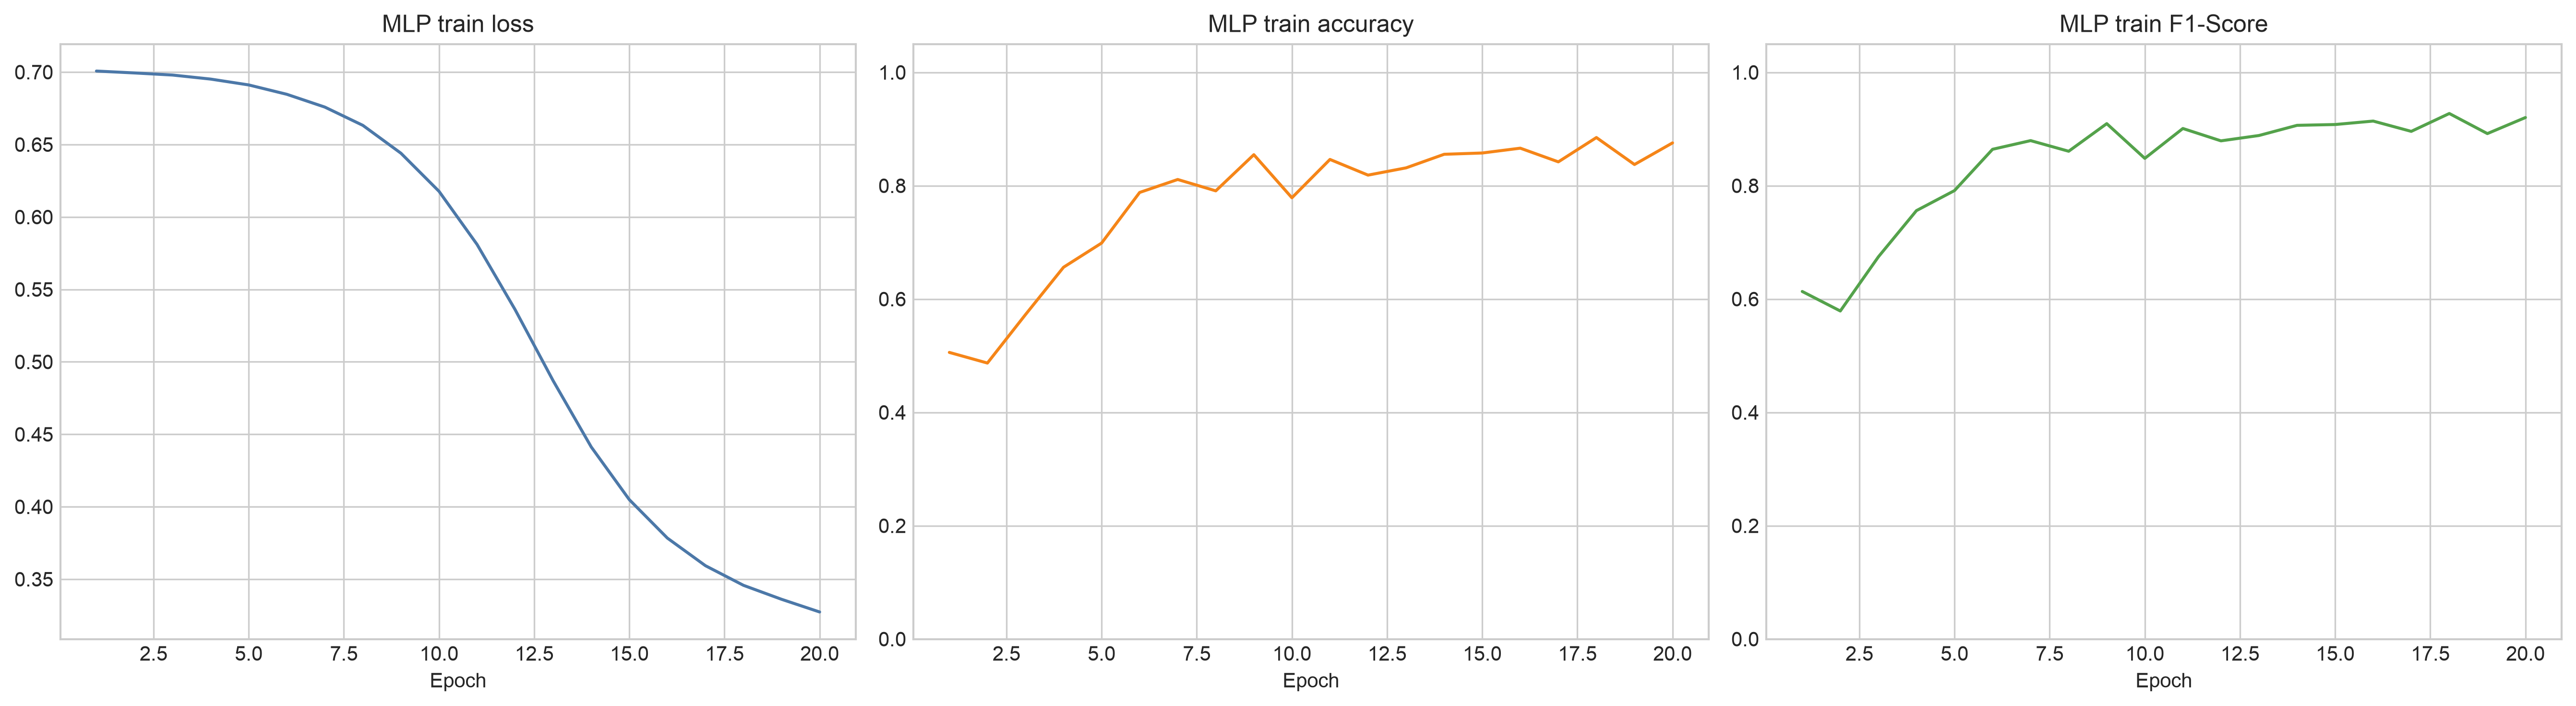
\includegraphics[width=0.95\textwidth]{customer_comments_mlp_learning_curve.png}
    \caption{Learning curve của MLP NumPy trên vector TF-IDF 1,000 chiều}
    \label{fig:comments_learning_curve}
\end{figure}

\section{So sánh trên tập test}
Multinomial Naive Bayes đạt F1 cao nhất, trong khi Logistic Regression đạt ROC-AUC cao nhất. Đây là kết quả hợp lý với văn bản TF-IDF thưa chiều cao, nơi các từ khóa sentiment tạo tín hiệu tuyến tính/xác suất rất mạnh.

\subsection{Đọc ma trận nhầm lẫn chuẩn hóa}
Ma trận nhầm lẫn chuẩn hóa trong Hình \ref{fig:comments_confusion} giúp so sánh mô hình khi số mẫu giữa hai lớp không bằng nhau.
Thay vì chỉ nhìn số lượng tuyệt đối, mỗi hàng được chuẩn hóa theo tổng số mẫu thật của lớp đó.
Điều này cho thấy mô hình bỏ sót bao nhiêu phần trăm review không khuyến nghị và khuyến nghị.

Trong bài toán thương mại điện tử, false positive nghĩa là mô hình dự đoán khách hàng sẽ khuyến nghị dù thực tế không khuyến nghị.
False negative nghĩa là mô hình bỏ sót một review tích cực.
Tùy mục tiêu nghiệp vụ, doanh nghiệp có thể ưu tiên phát hiện review tiêu cực để chăm sóc khách hàng, hoặc ưu tiên nhận diện review tích cực để khai thác tín hiệu marketing.

\begin{table}[H]
\centering
\caption{Benchmark 4 mô hình phân loại customer comments}
\label{tab:comments_benchmark}
\resizebox{\textwidth}{!}{%
\begin{tabular}{lccccccc}
\toprule
\textbf{Mô hình} & \textbf{Accuracy} & \textbf{Precision} & \textbf{Recall} & \textbf{F1-Score} & \textbf{ROC-AUC} & \textbf{Train(s)} & \textbf{Predict(s)} \\
\midrule
Multinomial Naive Bayes & 0.8618 & 0.8643 & \textbf{0.9860} & \textbf{0.9212} & 0.9299 & \textbf{0.0020} & 0.0007 \\
Logistic Regression & \textbf{0.8686} & \textbf{0.9659} & 0.8703 & 0.9156 & \textbf{0.9348} & 0.0222 & \textbf{0.0005} \\
NumPy MLP (1000-64-16-1) & 0.8591 & 0.9640 & 0.8601 & 0.9091 & 0.9297 & 0.6906 & 0.0019 \\
Random Forest & 0.8527 & 0.9353 & 0.8811 & 0.9074 & 0.9016 & 0.9528 & 0.0253 \\
\bottomrule
\end{tabular}%
}
\end{table}

\begin{figure}[H]
    \centering
    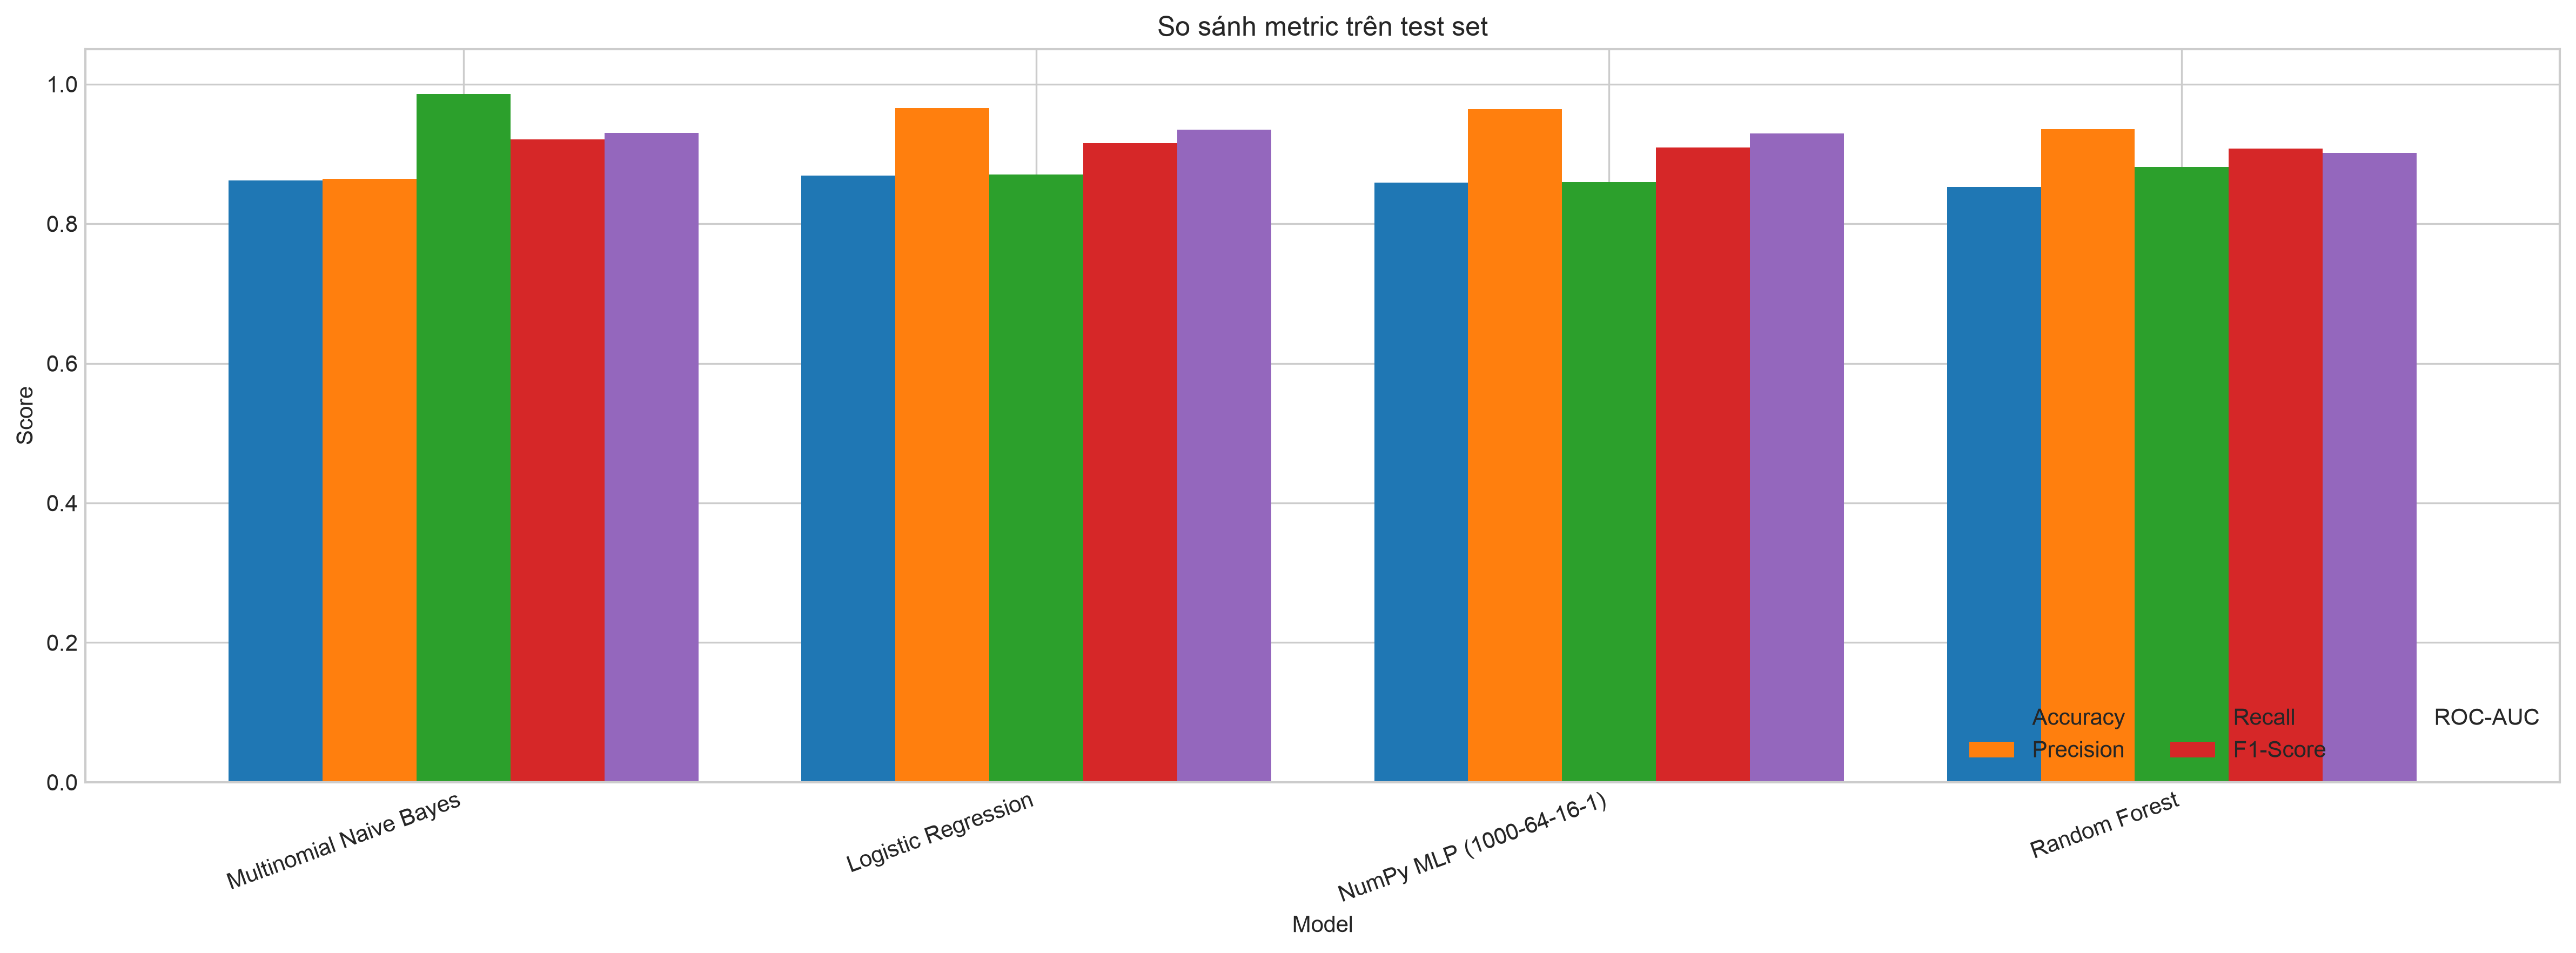
\includegraphics[width=\textwidth]{customer_comments_metric_comparison.png}
    \caption{So sánh đa chỉ số trên customer comments}
    \label{fig:comments_metric_comparison}
\end{figure}

\begin{figure}[H]
    \centering
    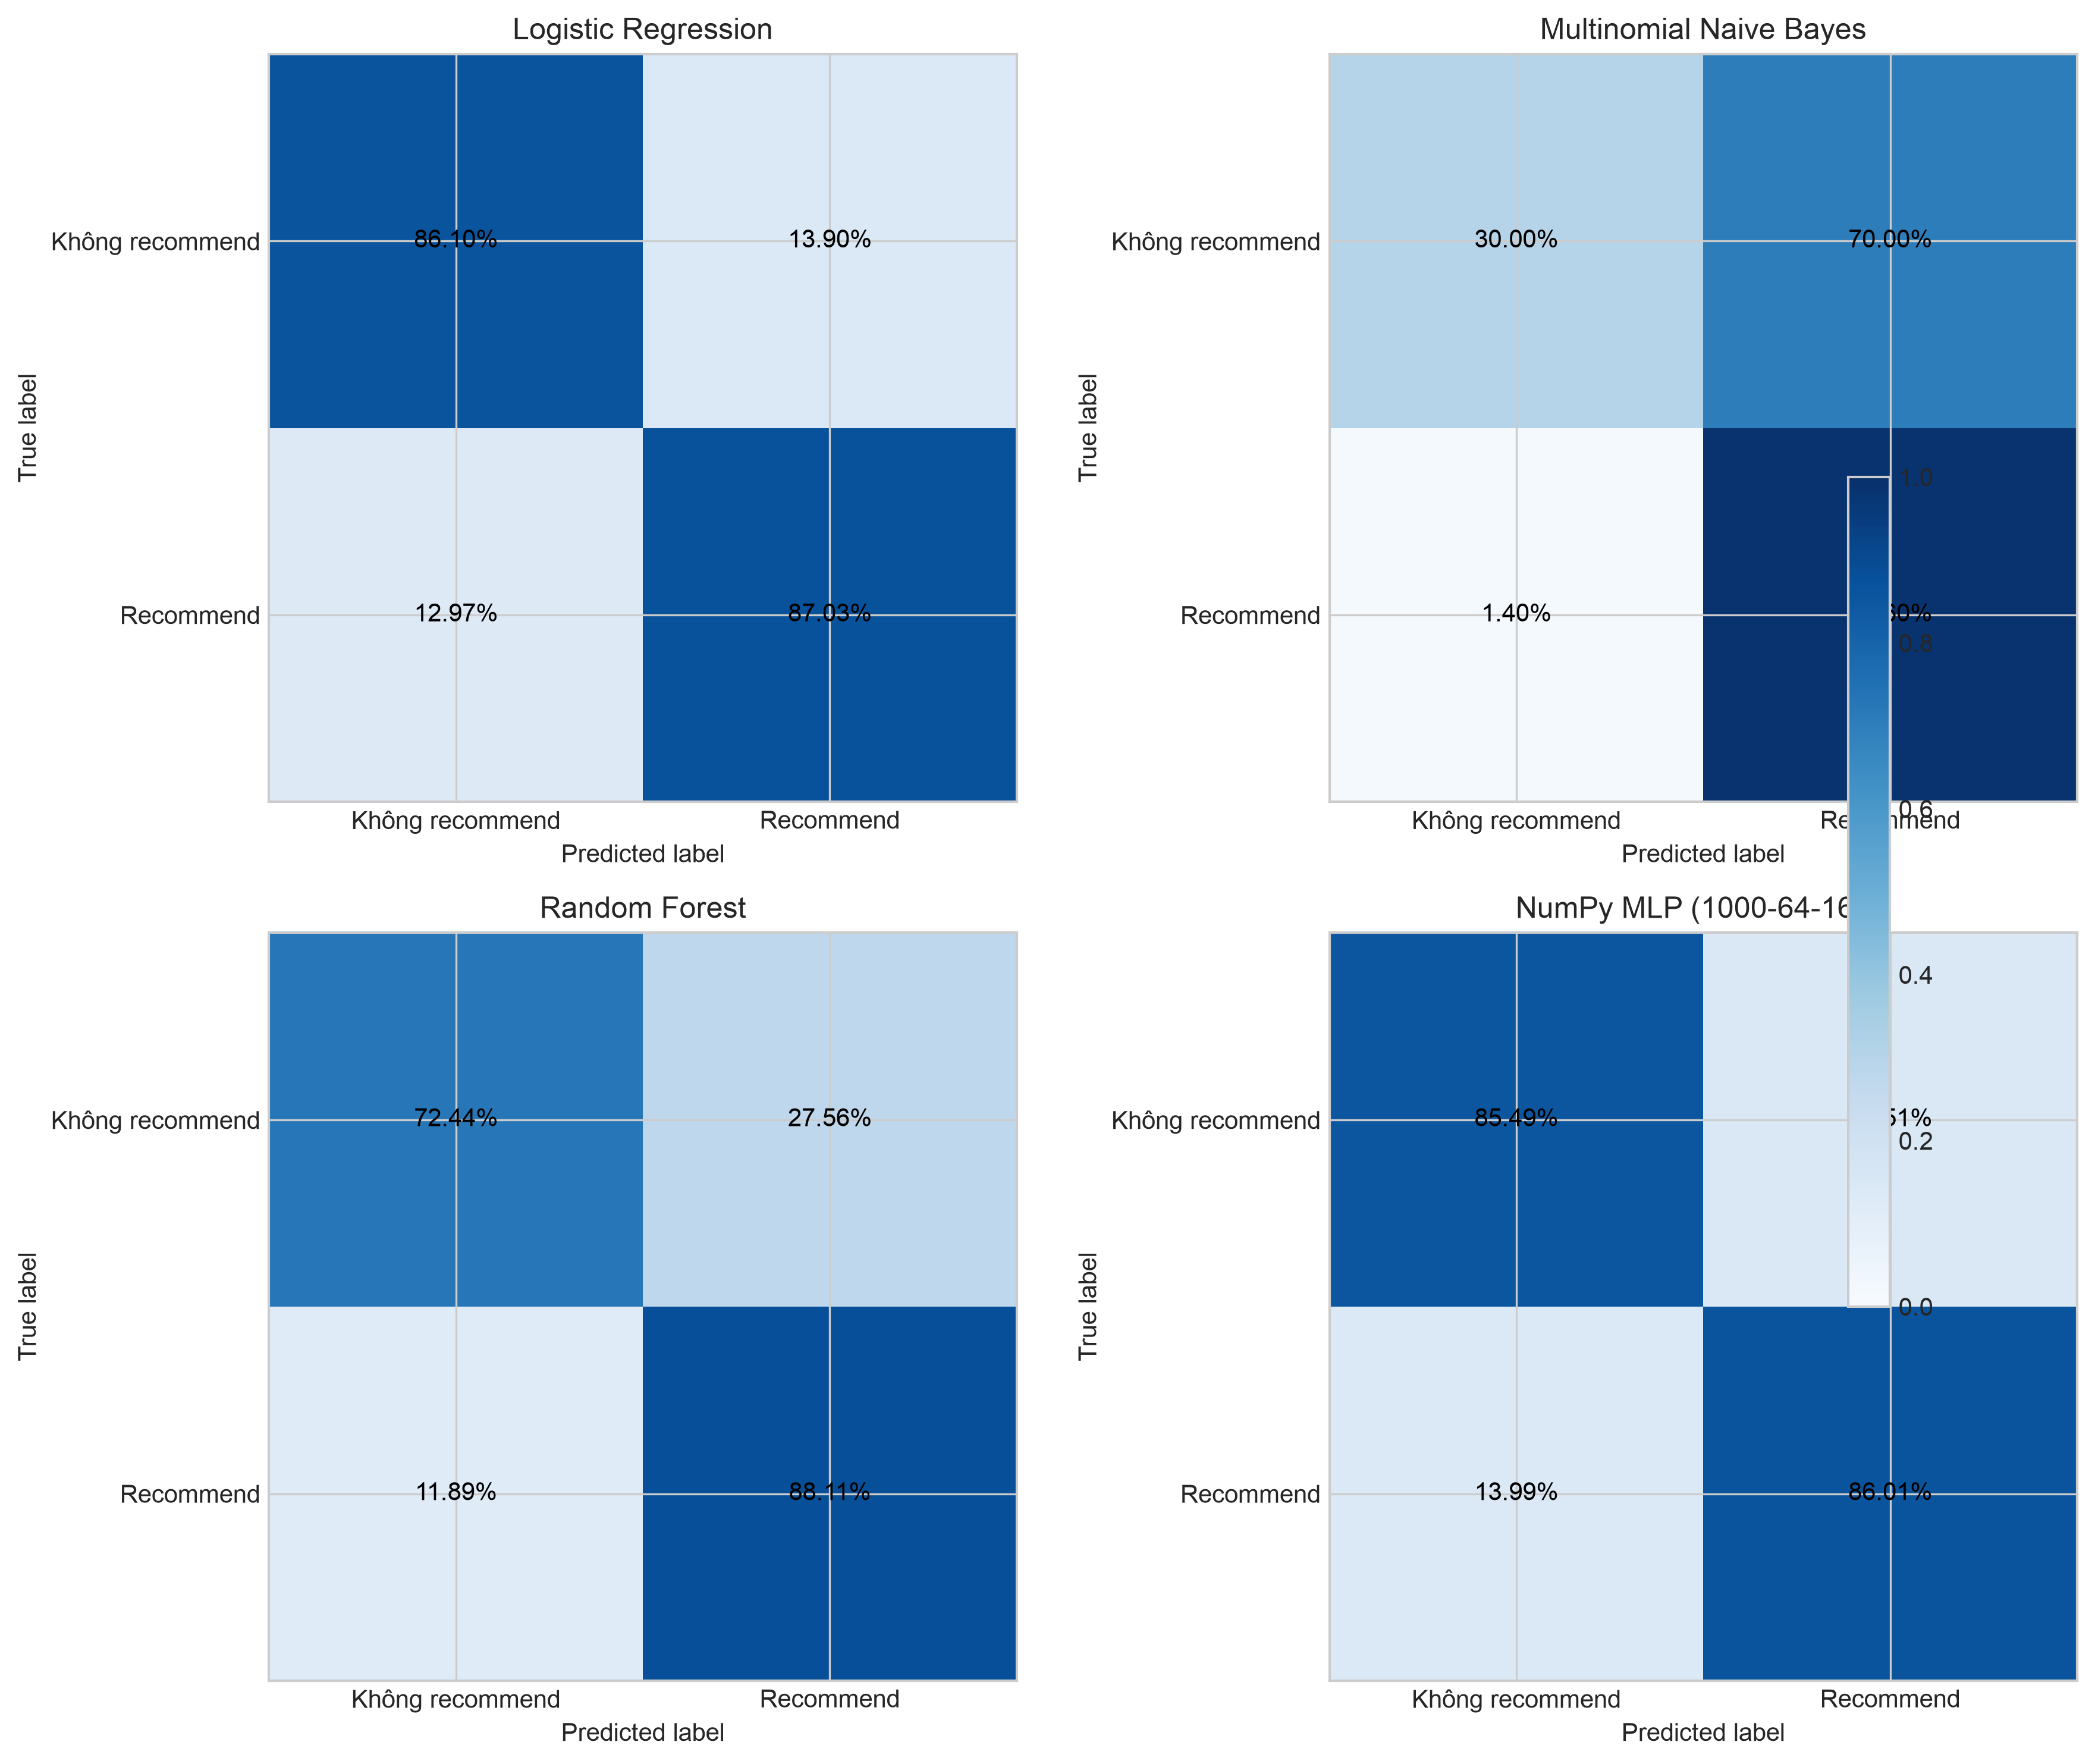
\includegraphics[width=\textwidth]{customer_comments_normalized_confusion_matrices.png}
    \caption{Ma trận nhầm lẫn chuẩn hóa của 4 mô hình phân loại nhận xét}
    \label{fig:comments_confusion}
\end{figure}

% =========================================================================
% CHUONG 6
% =========================================================================
\chapter{Đối Chiếu Kết Quả Và Khả Năng Tái Lập}

\section{Kết quả chính theo từng notebook}
Bảng \ref{tab:master_summary} đặt cạnh nhau các mô hình đứng đầu theo metric được notebook sử dụng để sắp hạng. Không có một cấu hình duy nhất đứng đầu cả bốn thực nghiệm.

\begin{table}[H]
\centering
\caption{Tổng hợp kết quả chính của Assignment 03}
\label{tab:master_summary}
\resizebox{\textwidth}{!}{%
\begin{tabular}{lllll}
\toprule
\textbf{Hệ thống} & \textbf{Mô hình đứng đầu} & \textbf{Kết quả chính} & \textbf{Metric chính} & \textbf{Dạng dữ liệu} \\
\midrule
Customer comments & Naive Bayes / Logistic Reg. & F1 0.9212, ROC-AUC 0.9348 & F1 / ROC-AUC & Văn bản TF-IDF, 22,642 mẫu \\
House price & NumPy MLP & RMSLE 0.6578, MAE \$217,538 & RMSLE / MAE & Bảng bất động sản, sample 200,000 \\
Diabetes nhỏ & Improved MLP & F1 0.8358, Recall 0.9655 & F1 / Recall & Bảng y sinh, 768 mẫu \\
Diabetes large & Decision Tree & F1 0.8039, PR-AUC 0.8514 & F1 / PR-AUC & Bảng y sinh, 100,000 mẫu \\
\bottomrule
\end{tabular}%
}
\end{table}

\section{Thảo luận kỹ thuật}
Trên dữ liệu bảng y sinh lớn, Decision Tree đạt hiệu quả cao nhờ khả năng tách ngưỡng tự nhiên như HbA1c hoặc blood glucose. Logistic Regression vẫn là baseline mạnh và nhanh, nhưng khó bắt các tương tác phi tuyến. Gaussian Naive Bayes có recall cao nhưng precision thấp do giả định độc lập đặc trưng quá mạnh.

Trên house price, MLP đứng đầu bảng theo RMSLE, MAE và $R^2$. Notebook huấn luyện mô hình trên \texttt{log1p(price)}, dùng các đặc trưng số, one-hot, frequency encoding và đặc trưng trích xuất từ \texttt{prev\_sold\_date}.

Trên customer comments, Naive Bayes và Logistic Regression nổi bật vì TF-IDF tạo không gian thưa có nhiều tín hiệu tuyến tính. MLP NumPy bám khá sát hai mô hình truyền thống, cho thấy mạng học được biểu diễn phi tuyến, nhưng chi phí huấn luyện cao hơn và chưa vượt baseline cổ điển trong bài toán text đơn giản.

\subsection{Ưu và nhược điểm theo nhóm mô hình}
Bảng \ref{tab:model_tradeoff} tóm tắt trade-off của các nhóm mô hình xuất hiện trong báo cáo.
Đây là phần quan trọng khi chuyển từ điểm số benchmark sang quyết định chọn mô hình.
Một mô hình có F1 cao nhất chưa chắc là lựa chọn duy nhất nếu hệ thống cần giải thích tốt, huấn luyện rất nhanh hoặc triển khai trên môi trường hạn chế tài nguyên.

\begin{table}[H]
\centering
\caption{Ưu và nhược điểm của các nhóm mô hình trong Assignment 03}
\label{tab:model_tradeoff}
\resizebox{\textwidth}{!}{%
\begin{tabular}{llll}
\toprule
\textbf{Nhóm mô hình} & \textbf{Ưu điểm} & \textbf{Nhược điểm} & \textbf{Phù hợp nhất trong báo cáo} \\
\midrule
Logistic/Ridge Regression & Nhanh, ổn định, dễ giải thích & Khó học tương tác phi tuyến mạnh & Baseline bảng và TF-IDF \\
Naive Bayes & Rất nhanh, hiệu quả với text sparse & Giả định độc lập feature đơn giản & Customer comments \\
Decision Tree/Random Forest & Học ngưỡng và tương tác phi tuyến & Có thể overfit, giải thích forest khó hơn tree đơn & Diabetes large, house price baseline \\
NumPy MLP & Học biểu diễn phi tuyến, kiểm soát rõ thuật toán & Tốn công cài đặt, nhạy hyperparameter, train lâu hơn & House price, minh họa deep learning thuần NumPy \\
\bottomrule
\end{tabular}%
}
\end{table}

\subsection{Hiệu năng, thời gian và khả năng giải thích}
Các kết quả cho thấy tốc độ và chất lượng không luôn đi cùng nhau.
Gaussian Naive Bayes trên diabetes large huấn luyện nhanh nhất nhưng precision thấp.
Multinomial Naive Bayes trên customer comments vừa nhanh vừa đạt F1 cao nhất vì cấu trúc bài toán phù hợp với giả định của mô hình.
Trong khi đó, MLP trên house price tốn thời gian hơn Ridge Regression nhưng đạt RMSLE và MAE tốt hơn.

Khả năng giải thích cũng khác nhau theo mô hình.
Logistic Regression và Ridge cho phép đọc dấu và độ lớn hệ số sau khi feature đã chuẩn hóa.
Decision Tree có thể diễn giải bằng các nhánh quyết định.
Random Forest cung cấp feature importance nhưng khó giải thích từng dự đoán.
MLP NumPy cho phép hiểu thuật toán ở mức ma trận và gradient, nhưng diễn giải từng trọng số trực tiếp khó hơn mô hình tuyến tính.

\section{Đối chiếu khả năng tái lập}
Các notebook đều cố định \texttt{RANDOM\_STATE = 42}, dùng split rõ ràng và fit các bước tiền xử lý chỉ trên training set. Những notebook sinh đồ thị lưu ảnh vào \modelpath{report/figures} tương ứng; bản ảnh được báo cáo sử dụng nằm trong \modelpath{Assignment3/Report/images/generated}.

\subsection{Checklist tái lập}
Bảng \ref{tab:reproducibility_checklist} ghi lại các điều kiện chính để người đọc có thể chạy lại notebook và đối chiếu báo cáo.
Checklist này đặc biệt hữu ích vì báo cáo dùng nhiều dataset, nhiều mô hình và nhiều thư mục hình khác nhau.

\begin{table}[H]
\centering
\caption{Checklist tái lập thực nghiệm}
\label{tab:reproducibility_checklist}
\resizebox{\textwidth}{!}{%
\begin{tabular}{lll}
\toprule
\textbf{Hạng mục} & \textbf{Cách thực hiện trong notebook} & \textbf{Ý nghĩa} \\
\midrule
Random seed & \texttt{RANDOM\_STATE = 42} & Giảm dao động do split và khởi tạo \\
Split dữ liệu & Stratified split cho phân loại, split riêng cho hồi quy & Giữ test set độc lập \\
Tiền xử lý & Fit scaler/encoder/vectorizer trên train & Chống data leakage \\
MLP NumPy & Theo dõi train/validation loss & Phát hiện overfitting và chọn epoch \\
Đánh giá & Dùng nhiều metric và confusion matrix & Tránh kết luận lệch từ một chỉ số \\
Hình ảnh & Lưu bằng \texttt{save\_current\_figure(...)} trước \texttt{plt.show()} & Bảo đảm báo cáo LaTeX có đủ hình \\
\bottomrule
\end{tabular}%
}
\end{table}

\subsection{Danh sách notebook nguồn}
Các kết quả trong báo cáo được lấy từ các notebook sau.
Mỗi notebook vừa hiển thị biểu đồ trực tiếp, vừa lưu bản PNG vào thư mục \modelpath{report/figures} tương ứng.
Khi cần kiểm tra lại kết quả, nên chạy notebook từ chính thư mục \modelpath{notebook} để đường dẫn tương đối tới \modelpath{../data} hoạt động đúng.

\begin{itemize}
    \item \modelpath{Assignment3/diabetes/notebook/diabetes\_improved.ipynb}
    \item \modelpath{Assignment3/diabetes\_large/notebook/diabetes\_large\_benchmark.ipynb}
    \item \modelpath{Assignment3/house\_price/notebook/house\_price\_benchmark.ipynb}
    \item \modelpath{Assignment3/customer\_comments/notebook/customer\_comments\_benchmark.ipynb}
\end{itemize}

\section{Kết luận}
Báo cáo đối chiếu MLP thuần NumPy trên bốn thực nghiệm: diabetes nhỏ, diabetes large, house price và customer comments. Các output trong notebook cho thấy:
\begin{enumerate}
    \item MLP thuần NumPy giúp hiểu rõ cơ chế forward/backward và vai trò của learning rate, regularization, batch size.
    \item Mô hình truyền thống vẫn rất cạnh tranh, đặc biệt trên dữ liệu TF-IDF và dữ liệu bảng có ngưỡng phân tách rõ.
    \item Với dữ liệu mất cân bằng, F1, recall, ROC-AUC và PR-AUC quan trọng hơn accuracy đơn thuần.
    \item Với hồi quy giá nhà, cần ưu tiên RMSLE/MAE và phân tích residual thay vì chỉ nhìn $R^2$.
\end{enumerate}

\end{document}
